% Options for packages loaded elsewhere
\PassOptionsToPackage{unicode}{hyperref}
\PassOptionsToPackage{hyphens}{url}
\PassOptionsToPackage{dvipsnames,svgnames,x11names}{xcolor}
%
\documentclass[
  letterpaper,
  DIV=11,
  numbers=noendperiod]{scrartcl}

\usepackage{amsmath,amssymb}
\usepackage{iftex}
\ifPDFTeX
  \usepackage[T1]{fontenc}
  \usepackage[utf8]{inputenc}
  \usepackage{textcomp} % provide euro and other symbols
\else % if luatex or xetex
  \usepackage{unicode-math}
  \defaultfontfeatures{Scale=MatchLowercase}
  \defaultfontfeatures[\rmfamily]{Ligatures=TeX,Scale=1}
\fi
\usepackage{lmodern}
\ifPDFTeX\else  
    % xetex/luatex font selection
\fi
% Use upquote if available, for straight quotes in verbatim environments
\IfFileExists{upquote.sty}{\usepackage{upquote}}{}
\IfFileExists{microtype.sty}{% use microtype if available
  \usepackage[]{microtype}
  \UseMicrotypeSet[protrusion]{basicmath} % disable protrusion for tt fonts
}{}
\makeatletter
\@ifundefined{KOMAClassName}{% if non-KOMA class
  \IfFileExists{parskip.sty}{%
    \usepackage{parskip}
  }{% else
    \setlength{\parindent}{0pt}
    \setlength{\parskip}{6pt plus 2pt minus 1pt}}
}{% if KOMA class
  \KOMAoptions{parskip=half}}
\makeatother
\usepackage{xcolor}
\setlength{\emergencystretch}{3em} % prevent overfull lines
\setcounter{secnumdepth}{-\maxdimen} % remove section numbering
% Make \paragraph and \subparagraph free-standing
\ifx\paragraph\undefined\else
  \let\oldparagraph\paragraph
  \renewcommand{\paragraph}[1]{\oldparagraph{#1}\mbox{}}
\fi
\ifx\subparagraph\undefined\else
  \let\oldsubparagraph\subparagraph
  \renewcommand{\subparagraph}[1]{\oldsubparagraph{#1}\mbox{}}
\fi

\usepackage{color}
\usepackage{fancyvrb}
\newcommand{\VerbBar}{|}
\newcommand{\VERB}{\Verb[commandchars=\\\{\}]}
\DefineVerbatimEnvironment{Highlighting}{Verbatim}{commandchars=\\\{\}}
% Add ',fontsize=\small' for more characters per line
\usepackage{framed}
\definecolor{shadecolor}{RGB}{241,243,245}
\newenvironment{Shaded}{\begin{snugshade}}{\end{snugshade}}
\newcommand{\AlertTok}[1]{\textcolor[rgb]{0.68,0.00,0.00}{#1}}
\newcommand{\AnnotationTok}[1]{\textcolor[rgb]{0.37,0.37,0.37}{#1}}
\newcommand{\AttributeTok}[1]{\textcolor[rgb]{0.40,0.45,0.13}{#1}}
\newcommand{\BaseNTok}[1]{\textcolor[rgb]{0.68,0.00,0.00}{#1}}
\newcommand{\BuiltInTok}[1]{\textcolor[rgb]{0.00,0.23,0.31}{#1}}
\newcommand{\CharTok}[1]{\textcolor[rgb]{0.13,0.47,0.30}{#1}}
\newcommand{\CommentTok}[1]{\textcolor[rgb]{0.37,0.37,0.37}{#1}}
\newcommand{\CommentVarTok}[1]{\textcolor[rgb]{0.37,0.37,0.37}{\textit{#1}}}
\newcommand{\ConstantTok}[1]{\textcolor[rgb]{0.56,0.35,0.01}{#1}}
\newcommand{\ControlFlowTok}[1]{\textcolor[rgb]{0.00,0.23,0.31}{#1}}
\newcommand{\DataTypeTok}[1]{\textcolor[rgb]{0.68,0.00,0.00}{#1}}
\newcommand{\DecValTok}[1]{\textcolor[rgb]{0.68,0.00,0.00}{#1}}
\newcommand{\DocumentationTok}[1]{\textcolor[rgb]{0.37,0.37,0.37}{\textit{#1}}}
\newcommand{\ErrorTok}[1]{\textcolor[rgb]{0.68,0.00,0.00}{#1}}
\newcommand{\ExtensionTok}[1]{\textcolor[rgb]{0.00,0.23,0.31}{#1}}
\newcommand{\FloatTok}[1]{\textcolor[rgb]{0.68,0.00,0.00}{#1}}
\newcommand{\FunctionTok}[1]{\textcolor[rgb]{0.28,0.35,0.67}{#1}}
\newcommand{\ImportTok}[1]{\textcolor[rgb]{0.00,0.46,0.62}{#1}}
\newcommand{\InformationTok}[1]{\textcolor[rgb]{0.37,0.37,0.37}{#1}}
\newcommand{\KeywordTok}[1]{\textcolor[rgb]{0.00,0.23,0.31}{#1}}
\newcommand{\NormalTok}[1]{\textcolor[rgb]{0.00,0.23,0.31}{#1}}
\newcommand{\OperatorTok}[1]{\textcolor[rgb]{0.37,0.37,0.37}{#1}}
\newcommand{\OtherTok}[1]{\textcolor[rgb]{0.00,0.23,0.31}{#1}}
\newcommand{\PreprocessorTok}[1]{\textcolor[rgb]{0.68,0.00,0.00}{#1}}
\newcommand{\RegionMarkerTok}[1]{\textcolor[rgb]{0.00,0.23,0.31}{#1}}
\newcommand{\SpecialCharTok}[1]{\textcolor[rgb]{0.37,0.37,0.37}{#1}}
\newcommand{\SpecialStringTok}[1]{\textcolor[rgb]{0.13,0.47,0.30}{#1}}
\newcommand{\StringTok}[1]{\textcolor[rgb]{0.13,0.47,0.30}{#1}}
\newcommand{\VariableTok}[1]{\textcolor[rgb]{0.07,0.07,0.07}{#1}}
\newcommand{\VerbatimStringTok}[1]{\textcolor[rgb]{0.13,0.47,0.30}{#1}}
\newcommand{\WarningTok}[1]{\textcolor[rgb]{0.37,0.37,0.37}{\textit{#1}}}

\providecommand{\tightlist}{%
  \setlength{\itemsep}{0pt}\setlength{\parskip}{0pt}}\usepackage{longtable,booktabs,array}
\usepackage{calc} % for calculating minipage widths
% Correct order of tables after \paragraph or \subparagraph
\usepackage{etoolbox}
\makeatletter
\patchcmd\longtable{\par}{\if@noskipsec\mbox{}\fi\par}{}{}
\makeatother
% Allow footnotes in longtable head/foot
\IfFileExists{footnotehyper.sty}{\usepackage{footnotehyper}}{\usepackage{footnote}}
\makesavenoteenv{longtable}
\usepackage{graphicx}
\makeatletter
\def\maxwidth{\ifdim\Gin@nat@width>\linewidth\linewidth\else\Gin@nat@width\fi}
\def\maxheight{\ifdim\Gin@nat@height>\textheight\textheight\else\Gin@nat@height\fi}
\makeatother
% Scale images if necessary, so that they will not overflow the page
% margins by default, and it is still possible to overwrite the defaults
% using explicit options in \includegraphics[width, height, ...]{}
\setkeys{Gin}{width=\maxwidth,height=\maxheight,keepaspectratio}
% Set default figure placement to htbp
\makeatletter
\def\fps@figure{htbp}
\makeatother

\KOMAoption{captions}{tableheading}
\makeatletter
\makeatother
\makeatletter
\makeatother
\makeatletter
\@ifpackageloaded{caption}{}{\usepackage{caption}}
\AtBeginDocument{%
\ifdefined\contentsname
  \renewcommand*\contentsname{Table of contents}
\else
  \newcommand\contentsname{Table of contents}
\fi
\ifdefined\listfigurename
  \renewcommand*\listfigurename{List of Figures}
\else
  \newcommand\listfigurename{List of Figures}
\fi
\ifdefined\listtablename
  \renewcommand*\listtablename{List of Tables}
\else
  \newcommand\listtablename{List of Tables}
\fi
\ifdefined\figurename
  \renewcommand*\figurename{Figure}
\else
  \newcommand\figurename{Figure}
\fi
\ifdefined\tablename
  \renewcommand*\tablename{Table}
\else
  \newcommand\tablename{Table}
\fi
}
\@ifpackageloaded{float}{}{\usepackage{float}}
\floatstyle{ruled}
\@ifundefined{c@chapter}{\newfloat{codelisting}{h}{lop}}{\newfloat{codelisting}{h}{lop}[chapter]}
\floatname{codelisting}{Listing}
\newcommand*\listoflistings{\listof{codelisting}{List of Listings}}
\makeatother
\makeatletter
\@ifpackageloaded{caption}{}{\usepackage{caption}}
\@ifpackageloaded{subcaption}{}{\usepackage{subcaption}}
\makeatother
\makeatletter
\@ifpackageloaded{tcolorbox}{}{\usepackage[skins,breakable]{tcolorbox}}
\makeatother
\makeatletter
\@ifundefined{shadecolor}{\definecolor{shadecolor}{rgb}{.97, .97, .97}}
\makeatother
\makeatletter
\makeatother
\makeatletter
\makeatother
\ifLuaTeX
  \usepackage{selnolig}  % disable illegal ligatures
\fi
\IfFileExists{bookmark.sty}{\usepackage{bookmark}}{\usepackage{hyperref}}
\IfFileExists{xurl.sty}{\usepackage{xurl}}{} % add URL line breaks if available
\urlstyle{same} % disable monospaced font for URLs
\hypersetup{
  colorlinks=true,
  linkcolor={blue},
  filecolor={Maroon},
  citecolor={Blue},
  urlcolor={Blue},
  pdfcreator={LaTeX via pandoc}}

\author{}
\date{}

\begin{document}
\ifdefined\Shaded\renewenvironment{Shaded}{\begin{tcolorbox}[enhanced, interior hidden, breakable, frame hidden, boxrule=0pt, borderline west={3pt}{0pt}{shadecolor}, sharp corners]}{\end{tcolorbox}}\fi

\hypertarget{non-covalent-functionalisation-of-carbon-nanotubes-and-graphene}{%
\section{Non-Covalent Functionalisation of Carbon Nanotubes and
Graphene}\label{non-covalent-functionalisation-of-carbon-nanotubes-and-graphene}}

\hypertarget{introduction}{%
\subsection{Introduction}\label{introduction}}

In previous chapters, I have discussed methods of fabricating carbon
nanotube and graphene devices and then shown that they are sensitive to
environmental changes in a saline solution. However, for specific
sensing, the devices require (bio)chemical functionalisation. Instead of
responding to stimuli themselves, the sensing signal is picked up by
attached receptors. The devices then act as passive transducers for the
received signal. Receptors previously used with carbon nanotube and
graphene devices include aptamers {[}@Khan2021; @Nguyen2021;
@Shkodra2021; @Nekrasov2021; @Mishyn2022; @Cassie2023{]} and a range of
proteins {[}@Lerner2014; @Ahn2020; @Tong2020; @Wang2020{]}, including
animal odorant receptors {[}@Goldsmith2011; @Lee2018; @Murugathas2019b;
@Murugathas2020; @Moon2020; @Yoo2022{]}. A common approach to attaching
receptors to the transducer involves the use of a linker molecule to
tether the receptor to the transducer. Verifying that this linker
molecule is bridging between the transducer and the receptor element is
important for a complete understanding of the behaviour of these
sensors. This verification involves providing evidence for effective
attachment of linker molecule to the transducing device channel, then
showing successful tethering of odorant receptors and other biomolecules
to the attached linker molecule.

This chapter therefore takes some time exploring the following selection
of available linker molecules for specific biosensing: 1-Pyrenebutanoic
Acid N-Hydroxysuccinimide Ester (PBASE), 1-Pyrenebutyric Acid (PBA),
Pyrene-PEG-NTA (PPN) and Pyrene-PEG-Biotin (PPB). The linker molecules
used are discussed in detail, and numerous hurdles to successful
functionalisation via linker molecules are identified and addressed.
Next, it looks at verifying that that the odorant receptor proteins of
interest have specifically attached to these linker molecules. The
experimental parameters used for both the attachment of linker molecules
and receptor proteins are also varied, and the impact of these
variations on successful functionalisation is investigated via Raman
spectroscopy, fluorescence microscopy and electrical characterisation.

\hypertarget{non-covalent-bonding-and-pi-stacking}{%
\subsection{\texorpdfstring{Non-Covalent Bonding and
\(\pi\)-Stacking}{Non-Covalent Bonding and \textbackslash pi-Stacking}}\label{non-covalent-bonding-and-pi-stacking}}

Linker molecules may be attached via covalent or non-covalent bonding to
carbon nanomaterials, such as carbon nanotubes and graphene. Covalent
bonding is stronger than non-covalent bonding, and therefore gives a
more permanent attachment between linker molecules and the transducer.
However, non-covalent bonding has the advantage of having less of an
impact on the structure of a nanomaterial than covalent bonding, meaning
non-covalent bonding is less likely to negatively affect the electrical
properties of the transducer {[}@Long2012; @DiCrescenzo2014; @Wang2020;
@Khan2021; @Mishyn2022{]}. For example, one group found covalent bonding
of diazonium linker caused a \(\sim 50\)\% drop in graphene channel
mobility {[}@Lerner2014{]}. In comparison, only a \(\sim 5\)\% drop in
mobility was seen for attachment of a mixture of linkers containing
pyrene to a graphene channel via non-covalent \(\pi\) stacking
{[}@Thodkar2021{]}.

\begin{figure}

{\centering 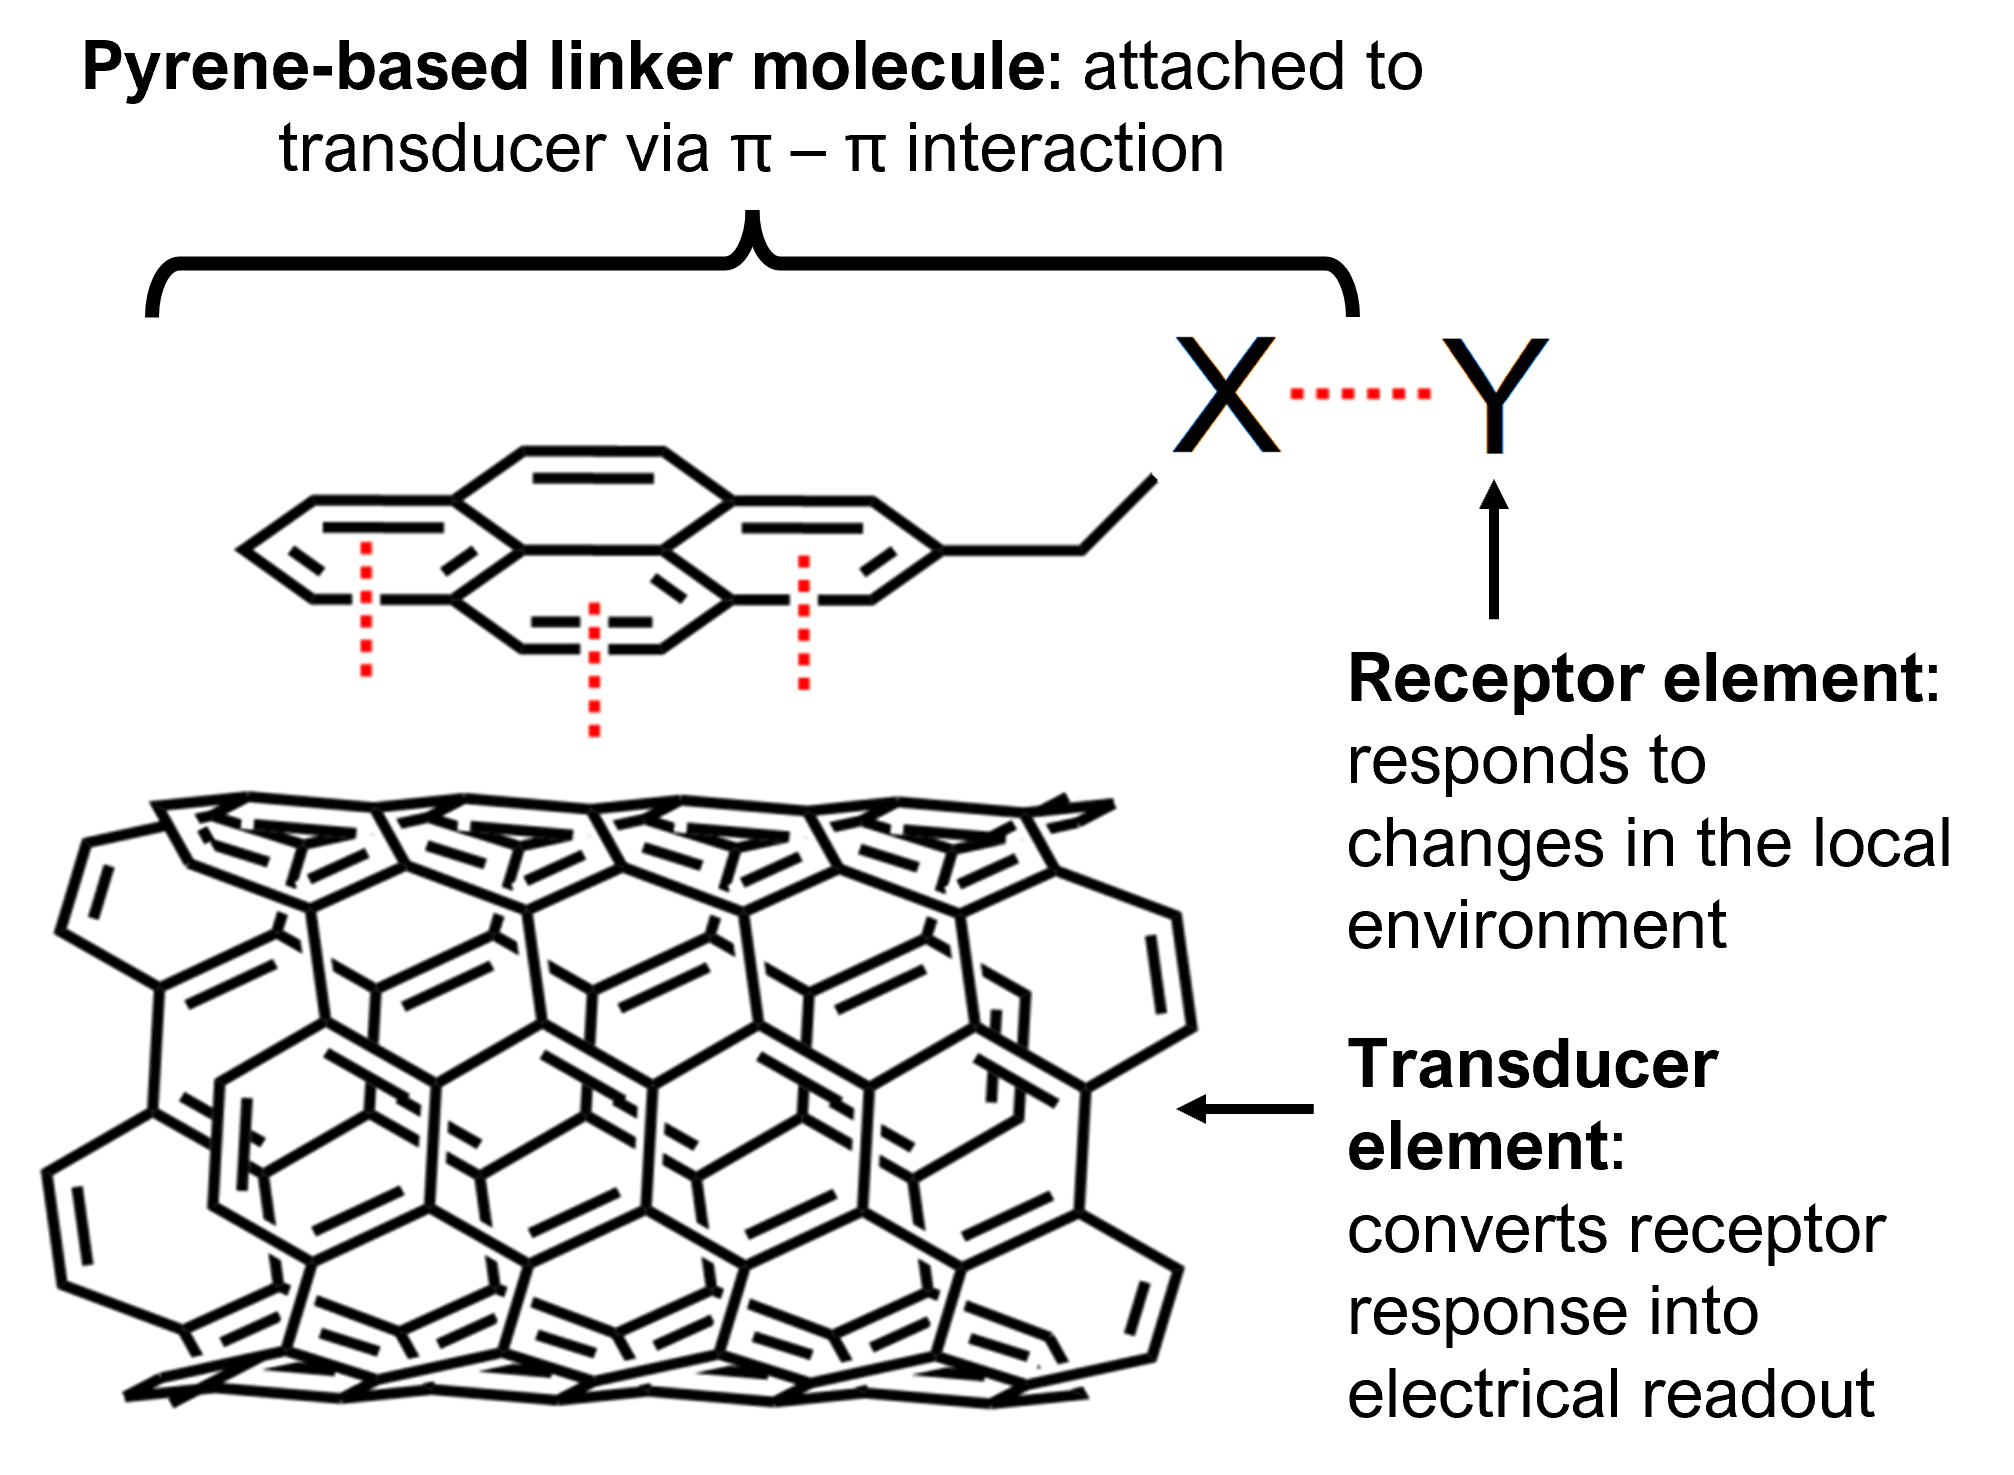
\includegraphics[width=0.8\textwidth,height=\textheight]{figures/ch7/pyrene-cnt.png}

}

\caption{\label{fig-pi-interaction-cnt}Attachment of pyrene-based linker
molecule pyrene-X and receptor Y to a carbon nanotube, representing the
transducer element of a field-effect transistor. Source: Adapted from
{[}@Carbonnanotube{]}.}

\end{figure}

\(\pi\)-stacking or \(\pi-\pi\) interaction is often used to describe a
type of non-covalent bonding which occurs due to dispersion forces
between unsaturated polycyclic molecules {[}@Perez2015{]}. It has been
argued that this label is unhelpfully specific and a misrepresentation
of what can be simply classed as a type of Van Der Waals bonding
{[}@Martinez2012; @Perez2015{]}. However, as the use of the term is
widespread in the literature, it is also used here for the sake of
clarity. Carbon nanotubes and graphene consist of a network of carbon
atoms attached to each other by sp\(^{2}\) hybrid orbitals in a
polycyclic structure. They are therefore able to strongly interact with
linker molecules with aromatic moieties, such as pyrene
{[}@Hermanson2013-16; @Perez2015; @Mishyn2022{]}.
Figure~\ref{fig-pi-interaction-cnt} is a visual demonstration of the
relationship between the pyrene-based linker molecule with the
transducer and receptor elements. A wide range of pyrene-based linker
molecules have been used for non-covalent modification of carbon
nanotubes and graphene {[}@Zhou2019{]}. \(\pi\)-stacking with pyrene is
the bonding mechanism underlying all the functionalisation processes in
this thesis.

\hypertarget{sec-PBASE}{%
\subsection{Attachment of 1-Pyrenebutanoic Acid N-Hydroxysuccinimide
Ester}\label{sec-PBASE}}

\hypertarget{comparing-attachment-methods}{%
\subsubsection{Comparing Attachment
Methods}\label{comparing-attachment-methods}}

\begin{figure}

\begin{minipage}[t]{0.47\linewidth}

{\centering 

\raisebox{-\height}{

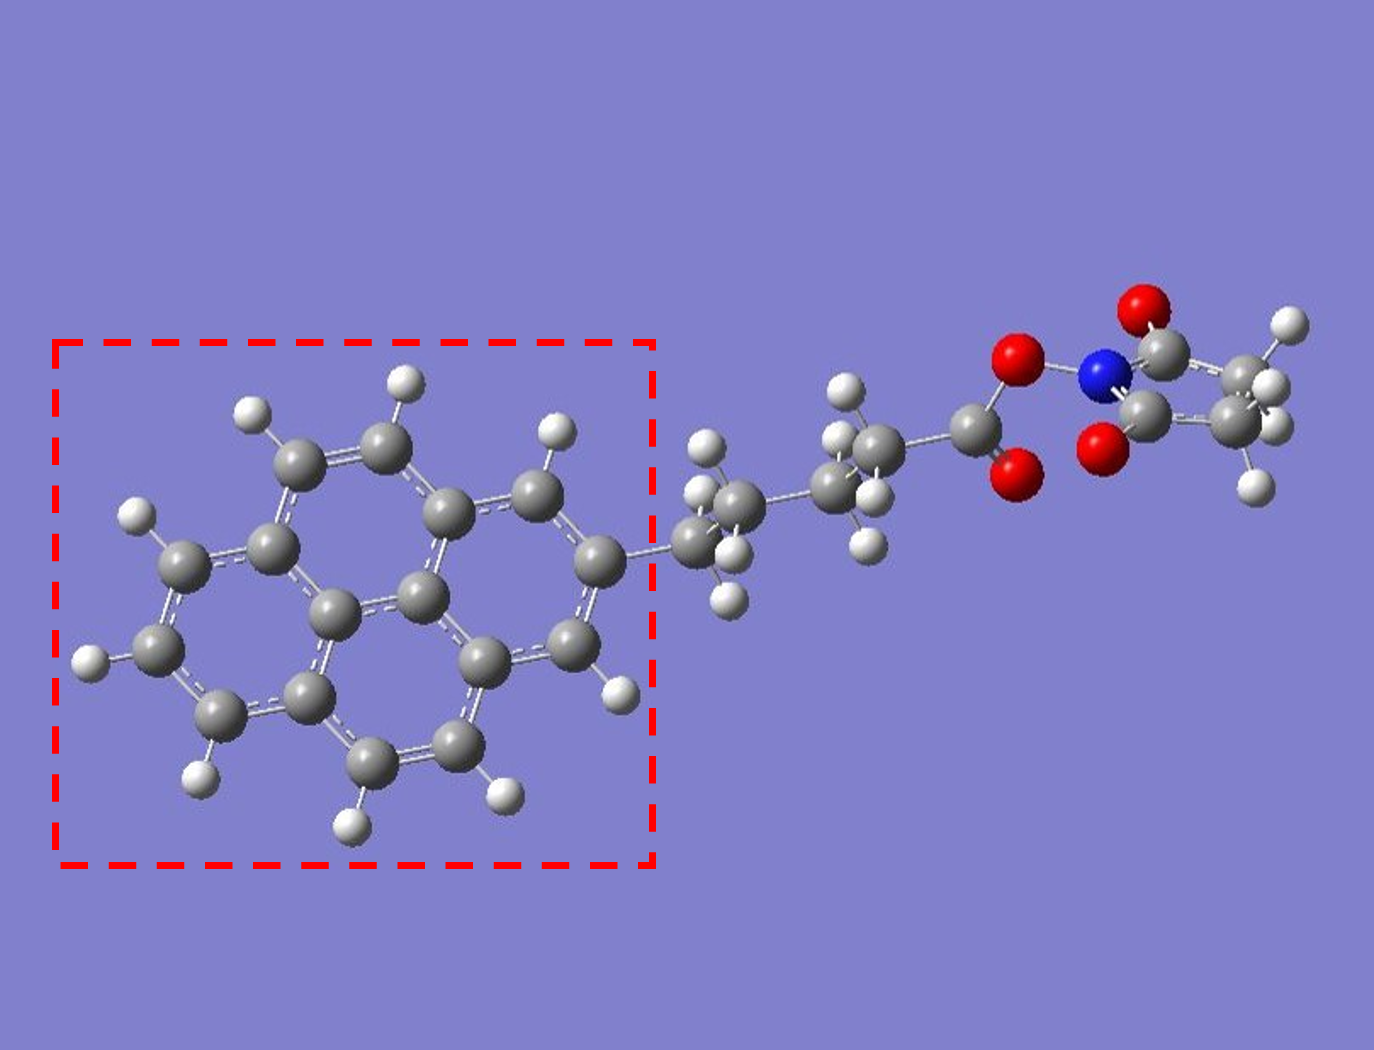
\includegraphics{figures/ch7/pbase_stable_1_pyrene.png}

}

}

\subcaption{\label{fig-pbase-stable-1}}
\end{minipage}%
%
\begin{minipage}[t]{0.05\linewidth}

{\centering 

~

}

\end{minipage}%
%
\begin{minipage}[t]{0.47\linewidth}

{\centering 

\raisebox{-\height}{

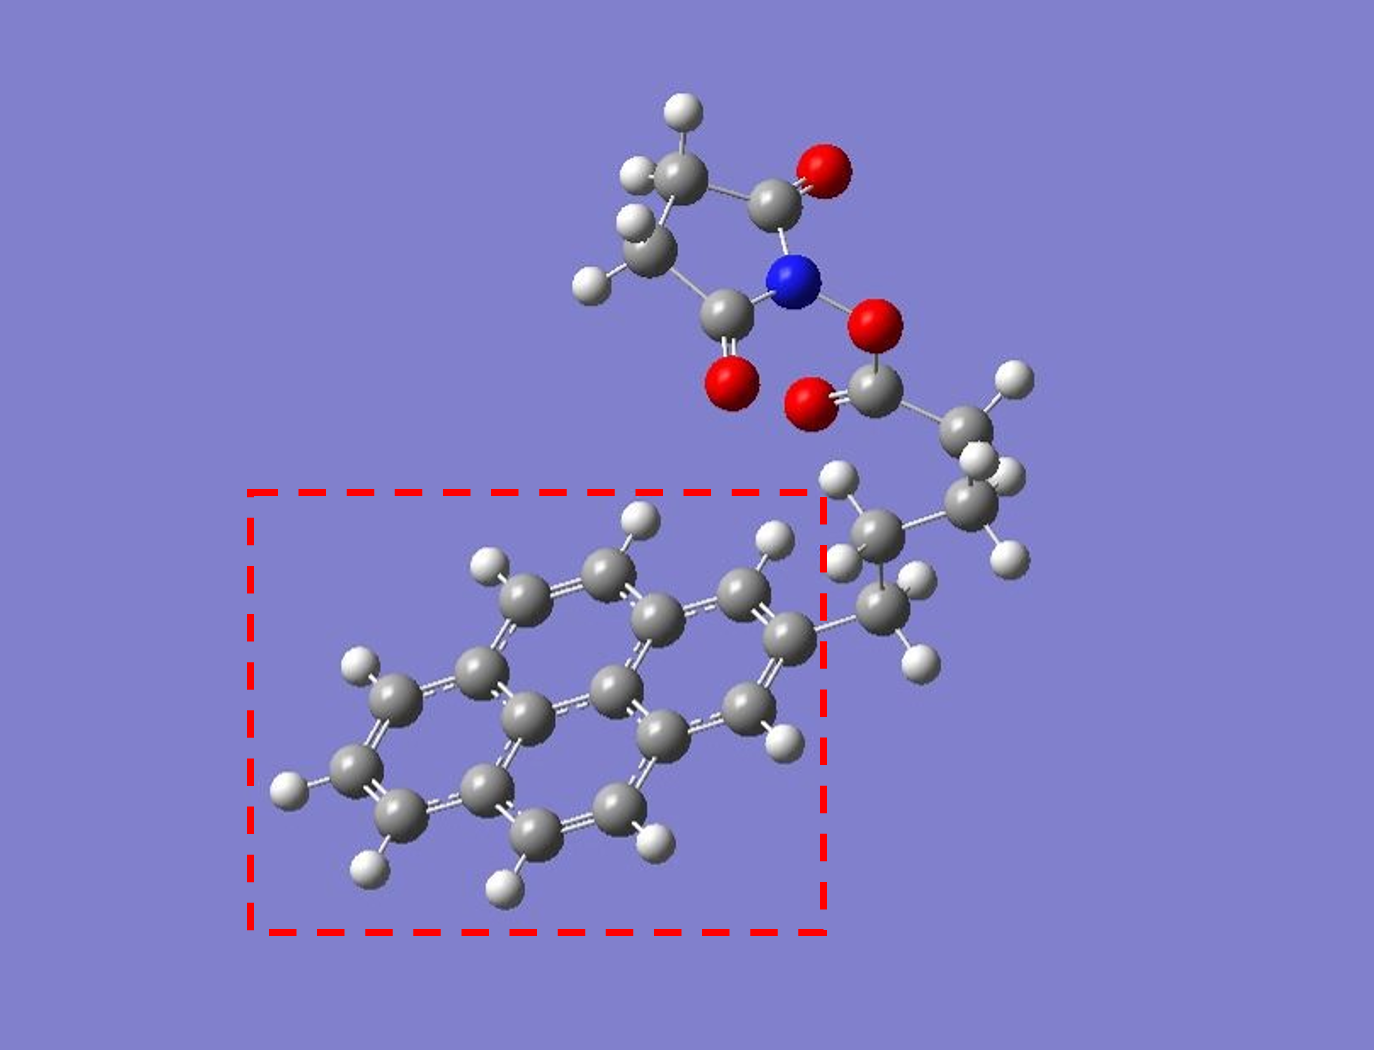
\includegraphics{figures/ch7/pbase_stable_2_pyrene.png}

}

}

\subcaption{\label{fig-pbase-stable-2}}
\end{minipage}%

\caption{\label{fig-pbase-structure}Two conformations of PBASE molecule
with geometry optimised via \emph{ab initio} calculations performed with
Gaussian 16 software {[}@g16{]}. White balls correspond to hydrogen,
grey to carbon, red to oxygen and blue to nitrogen. The pyrene moiety is
highlighted in the image with a red dashed outline.}

\end{figure}

1-pyrenebutanoic acid N-hydroxysuccinimide ester (also known
commercially and in the literature both as 1-pyrenebutyric acid
N-hydroxysuccinimide ester and 1-pyrenebutanoic acid succinimidyl ester;
acronyms include PBASE, PBSE, PyBASE, PASE, PYSE, PSE, Pyr-NHS and
PANHS) is a aromatic molecule commonly used for tethering biomolecules
to the carbon rings of graphene and carbon nanotubes. Using
computational modelling, two locally stable molecular conformations were
found to exist, a straight (Figure~\ref{fig-pbase-stable-1}) and bent
(Figure~\ref{fig-pbase-stable-2}) structure. The conformation in
Figure~\ref{fig-pbase-stable-1} has a Hartree-Fock energy of -3427728.67
kJ/mol, while the conformation in Figure~\ref{fig-pbase-stable-2} has a
Hartree-Fock energy of -3427729.66 kJ/mol. The difference between
computed Hartree-Fock energies is 1.0 kJ/mol, small enough that the
existence of both molecular conformations is physically feasible.
Similar straight and bent structures have previously been modelled for
PBASE attached to graphene {[}@Oishi2022{]}.

\newpage
\KOMAoptions{paper=landscape,pagesize}

\begin{Shaded}
\begin{Highlighting}[]
\NormalTok{knitr}\SpecialCharTok{::}\NormalTok{opts\_chunk}\SpecialCharTok{$}\FunctionTok{set}\NormalTok{(}\AttributeTok{echo =} \ConstantTok{FALSE}\NormalTok{)}
\FunctionTok{library}\NormalTok{(knitr)}

\NormalTok{pbase\_table }\OtherTok{\textless{}{-}} \FunctionTok{read.csv}\NormalTok{(}\StringTok{"tables/ch7/pbase\_table.csv"}\NormalTok{, }\AttributeTok{sep=}\StringTok{","}\NormalTok{)}
\NormalTok{pbase\_table }\OtherTok{\textless{}{-}}\NormalTok{ pbase\_table[}\FunctionTok{rowSums}\NormalTok{(}\FunctionTok{is.na}\NormalTok{(pbase\_table)) }\SpecialCharTok{==} \DecValTok{0}\NormalTok{,]}

\NormalTok{knitr}\SpecialCharTok{::}\FunctionTok{kable}\NormalTok{(pbase\_table, }
            \AttributeTok{col.names =} \FunctionTok{c}\NormalTok{(}\StringTok{"Solvent"}\NormalTok{,}
                           \StringTok{"Channel"}\NormalTok{,}
                           \StringTok{"Conc. (mM)"}\NormalTok{,}
                           \StringTok{"Incubation type"}\NormalTok{,}
                           \StringTok{"Time (hr)"}\NormalTok{,}
                           \StringTok{"Rinse steps"}\NormalTok{,}
                           \StringTok{"References"}\NormalTok{), }\AttributeTok{format =} \StringTok{"simple"}\NormalTok{) }
\end{Highlighting}
\end{Shaded}

\hypertarget{tbl-pbase-functionalisation}{}
\begin{longtable}[]{@{}lllllll@{}}
\caption{\label{tbl-pbase-functionalisation}Comparison of PBASE
functionalisation processes used for immobilisation of proteins and
aptamers onto carbon nanotubes and graphene. Experimentally optimised
variables are marked with a star (*). Blank entries indicate there was
no mention of the parameter in a particular paper.}\tabularnewline
\toprule\noalign{}
Solvent & Channel & Conc. (mM) & Incubation type & Time (hr) & Rinse
steps & References \\
\midrule\noalign{}
\endfirsthead
\toprule\noalign{}
Solvent & Channel & Conc. (mM) & Incubation type & Time (hr) & Rinse
steps & References \\
\midrule\noalign{}
\endhead
\bottomrule\noalign{}
\endlastfoot
DMF & CNT & 5 & Immersed & 1 & PBS & Maehashi, 2007.
\cite{Maehashi2007} \\
& & 6 & Immersed & 1 & DMF, PBS & García-Aljaro, 2010.
\cite{Garcia-Aljaro2010} \\
& & 6 & Immersed & 1 & DMF & Chen, 2001. \cite{Chen2001} \\
& & 6 & Immersed & 1 & DMF & Cella, 2010. \cite{Cella2010} \\
& & 6 & Immersed & 1 & DMF & Das, 2011. \cite{Das2011} \\
& & 6 & - & 2 & DMF & Besteman, 2003. \cite{Besteman2003} \\
& Graphene & - & - & 2 & DMF & Tsang, 2019. \cite{Tsang2019} \\
& & - & - & 20 & - & Wiedman, 2017. \cite{Wiedman2017} \\
& & 0.2 & Immersed & 20 & DMF, IPA, DI water & Gao, 2018.
\cite{Gao2018} \\
& & 1 & Dropcast & 6 & DMF, IPA, DI water & Nekrasov, 2021.
\cite{Nekrasov2021} \\
& & 5 & Immersed & 1 & DMF, DI water & Hwang, 2016. \cite{Hwang2016} \\
& & 5* & Immersed & 3* & DMF & Hao, 2020. \cite{Hao2020} \\
& & 5 & Immersed & 4* & DMF, DI water & Mishyn, 2022.
\cite{Mishyn2022} \\
& & 6 & Dropcast & 2 & DMF, DI water & Nur Nasufiya, 2020.
\cite{NurNasyifa2020} \\
& & 10 & Dropcast & 2 & DMF, DI water & Campos, 2019.
\cite{Campos2019} \\
& & 10 & Immersed & 2 & DMF, PBS & Kuscu, 2020. \cite{Kuscu2020} \\
& & 10 & Immersed & 1 & DMF & Xu, 2017. \cite{Xu2017} \\
& & 10 & Immersed & 12 & DMF, EtOH, DI water & Khan, 2020.
\cite{Khan2020} \\
& & 50 & Immersed & 4* & MeOH & Wang, 2020. \cite{Wang2020} \\
2-Methoxyethanol & Graphene & 1 & Immersed & 1 & DI water & Ono, 2020.
\cite{Ono2020} \\
Methanol & CNT & 1 & Immersed & 1 & MeOH, DI water & Zheng, 2016.
\cite{Zheng2016} \\
& & 1 & Immersed & 2 & MeOH & Kim, 2009. \cite{Kim2009} \\
& & 100 & Dropcast & 1 & DI water & Yoo, 2022. \cite{Yoo2022} \\
& Graphene & 5 & Immersed & 2 & - & Sethi, 2020. \cite{Sethi2020} \\
& & 5 & Immersed & 1 & MeOH, PBS & Ohno, 2010. \cite{Ohno2010} \\
DMSO & CNT & 10 & - & 1 & DI water & Lopez, 2015. \cite{Lopez2015} \\
& & 10 & Immersed & 1 & PBS & Strack, 2013. \cite{Strack2013} \\
\end{longtable}

\newpage
\KOMAoptions{paper=portrait,pagesize}

The pyrene moiety, highlighted with a red dashed outline in
Figure~\ref{fig-pbase-stable-1}-b, non-covalently bonds to the carbon
rings of the carbon nanotube and graphene surface. The
N-hydroxysuccinimide (NHS) ester group, seen on the right-hand side of
Figure~\ref{fig-pbase-structure}, is highly reactive with amine groups.
It can undergo a nucleophilic substitution reaction with amines attached
to proteins or aptamers, tethering these biomolecules via an amide or
imide bond {[}@Chen2001; @Hermanson2013-16; @Hermanson2013-3;
@Mishyn2022{]}.

The non-covalent functionalisation of proteins onto a single-walled
carbon nanotube using PBASE was first reported by Chen \emph{et al.} in
2001 {[}@Chen2001{]}. Two successful methods for protein
functionalisation and immobilisation were reported, with the only
differences being the solvent used to dissolve the PBASE powder (DMF,
methanol) and the final concentration of the resulting solutions (6 mM,
1 mM respectively). PBASE powder appears to dissolve poorly in methanol
at higher concentrations, which might explain the use of different
concentrations of PBASE in each solvent. An extensive comparison of
methods used in the literature for PBASE functionalisation of carbon
nanotube and graphene devices with aptamers and proteins is given in
Table~\ref{tbl-pbase-functionalisation}. Several listed works directly
cite Chen \emph{et al.} when discussing functionalisation with PBASE
{[}@Besteman2003; @Cella2010; @Campos2019; @Zheng2016; @Ohno2010{]}. The
other works listed do not explicitly reference Chen \emph{et al.} in
their methodology; however, the frequency of methods detailing the use
of 6 mM PBASE in dimethylformamide (DMF) and 1 mM PBASE in methanol
indicate that these processes are largely copying the process used by
Chen \emph{et al.}.

However, it is also apparent from
Table~\ref{tbl-pbase-functionalisation} that there is a large degree of
variation in the methods used for PBASE functionalisation. Various
electrical characterisation, microscopy and spectroscopy techniques have
been used to demonstrate successful functionalisation. Until recently,
there has been little justification provided for the selection of
variables used in the functionalisation procedure (e.g.~length of time
submerged in solvent containing PBASE), despite the wide-ranging use of
this process in the literature {[}@Hinnemo2017; @Zhen2018; @Wang2020{]}.
This is surprising, given that the sensitivity of functionalised devices
is considered to be closely related to the density of surface
functionalisation {[}@White2008; @Hermanson2013-3; @Chen2014{]}.
Furthermore, a detailed investigation of PBASE functionalisation process
variables has only been undertaken for graphene-based devices
{[}@Zhen2018; @Hao2020; @Wang2020; @Mishyn2022{]}.

Zhen \emph{et al.} {[}@Zhen2018{]}, Wang \emph{et al.} {[}@Wang2020{]}
and Mishyn \emph{et al.} {[}@Mishyn2022{]} have all claimed that
carefully tuning the surface concentration of PBASE is required to avoid
multilayer coverage of the graphene surface, as this negatively impacts
sensing. Mishyn \emph{et al.} {[}@Mishyn2022{]} used cyclic voltammetry
to demonstrate that less receptor attachment to the graphene surface
occurs when multiple layers of PBASE are present. However, none of these
groups have presented analyte sensing results from their functionalised
graphene devices. In contrast, Hao \emph{et al.} {[}@Hao2020{]} found
that maximising the PBASE surface coverage of a channel resulted in more
sensitive aptameric sensing, thereby reaching the opposite conclusion.
The inconsistency in these recent findings mean more work is needed to
understand the PBASE functionalisation process to achieve optimal
biosensor sensitivity. It may also be the case that a specific
functionalisation process is required for optimal sensitivity with the
use of a specific type of receptor.

\begin{figure}

\begin{minipage}[t]{\linewidth}

{\centering 

\raisebox{-\height}{

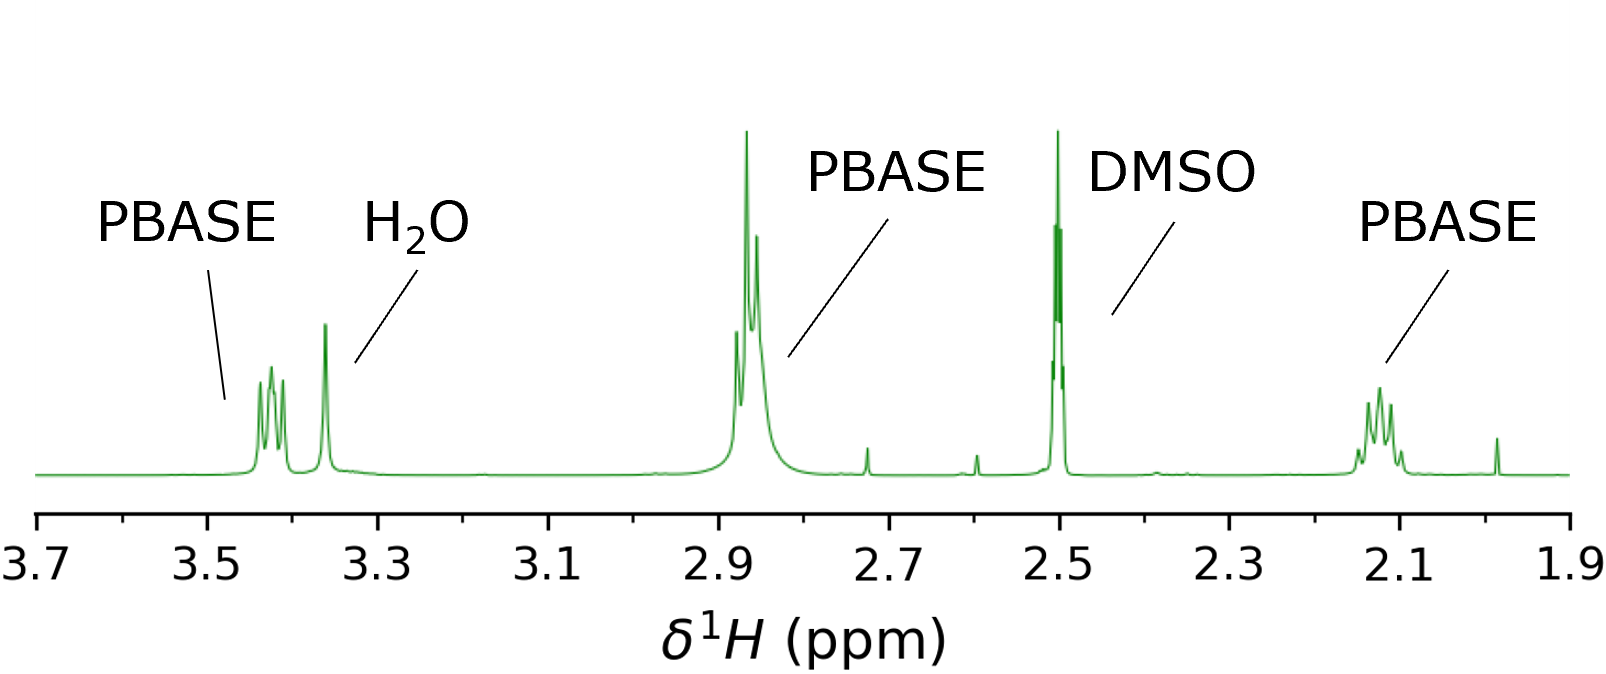
\includegraphics{figures/ch7/labelled_modified_sigma_pbase_nmr.png}

}

}

\subcaption{\label{fig-sigma-nmr}}
\end{minipage}%
\newline
\begin{minipage}[t]{\linewidth}

{\centering 

\raisebox{-\height}{

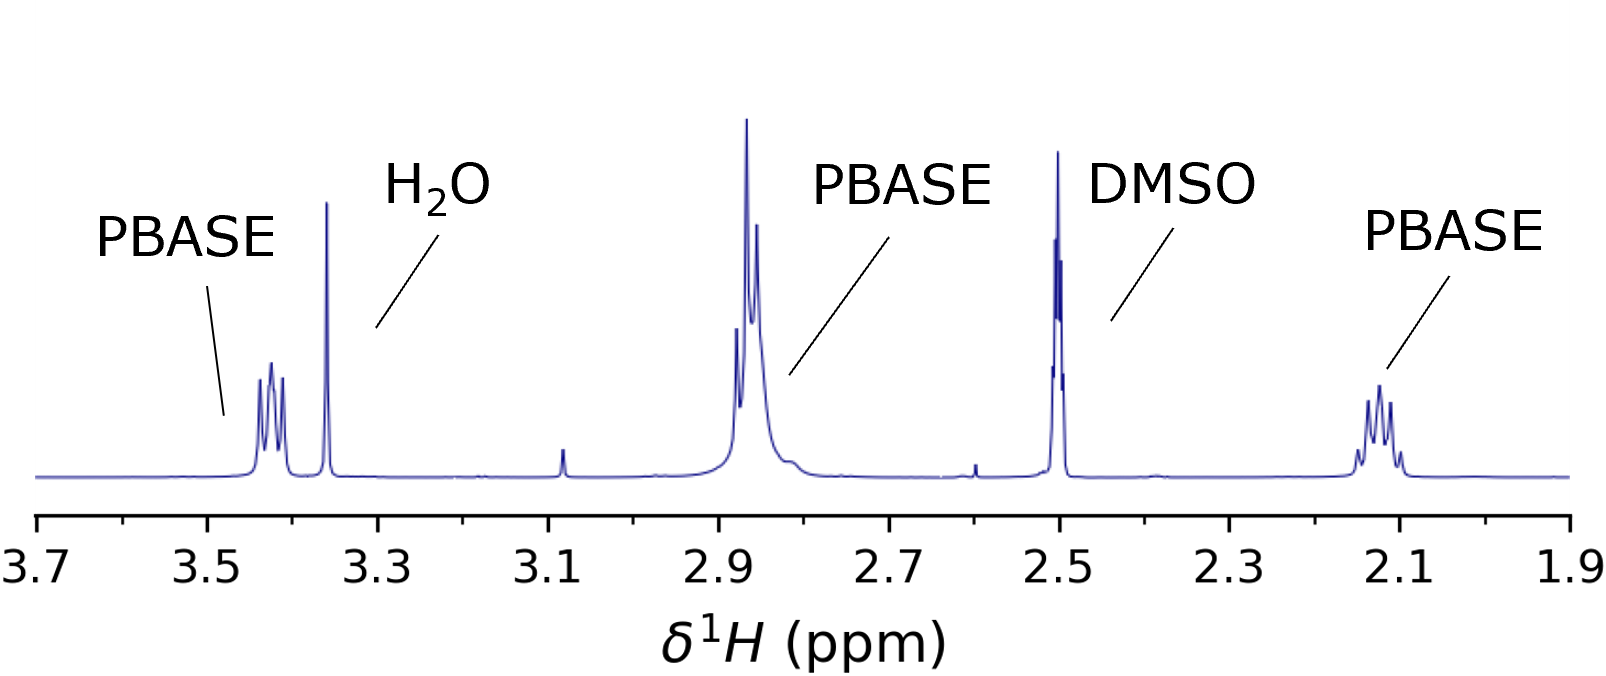
\includegraphics{figures/ch7/labelled_modified_setareh_pbase_nmr.png}

}

}

\subcaption{\label{fig-setareh-nmr}}
\end{minipage}%
\newline
\begin{minipage}[t]{\linewidth}

{\centering 

\raisebox{-\height}{

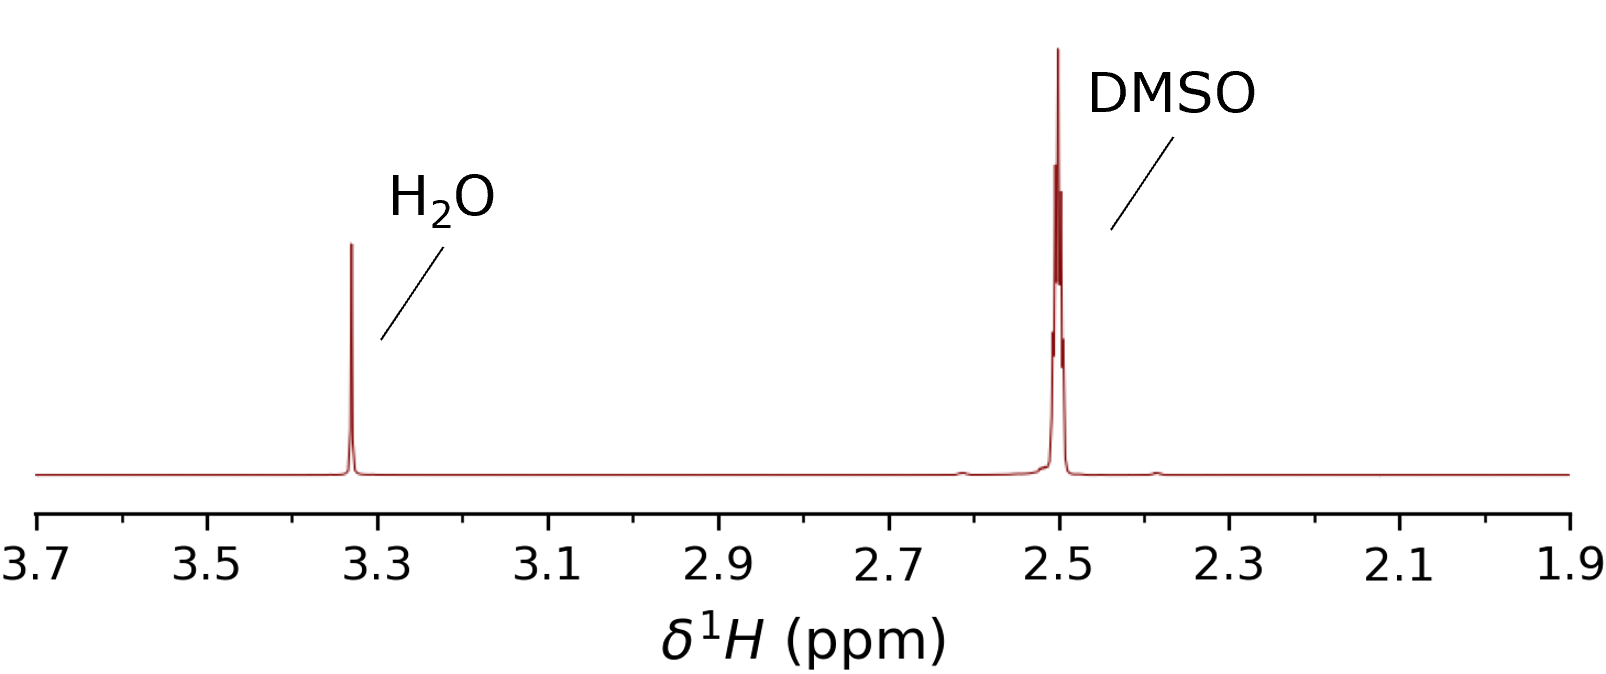
\includegraphics{figures/ch7/labelled_modified_dmso_nmr.png}

}

}

\subcaption{\label{fig-dmso-nmr}}
\end{minipage}%

\caption{\label{fig-pbase-nmr}\(^{1}\)H Nuclear Magnetic Resonance (NMR)
spectra, performed with DMSO-d\(_6\) used as the NMR solvent. (a) and
(b) show NMR spectrum for commercially purchased PBASE, from
Sigma-Aldrich and Setareh Biotech respectively, while (c) shows the
blank spectrum taken with only DMSO-d\(_6\) present. Spectra were taken
by Jennie Ramirez-Garcia, School of Chemical and Physical Sciences, Te
Herenga Waka - Victoria University of Wellington. Unlabelled peaks
correspond to sample impurities.}

\end{figure}

Once fastened to a bioreceptor via an amide or imide bond, the
attachment to the linker molecule is not easily broken. However, prior
to use in functionalisation processes, the NHS ester may react with any
water present (hydrolysis). This reaction converts PBASE to
1-pyrenebutyric acid (PBA), leaving it unavailable to react further with
amine groups {[}@Hermanson2013-3; @Hermanson2013-5; @Mishyn2022{]}. If
the amine group functionalisation is performed within a \(\sim1\) hour
period, with a high concentration of bioreceptor used at close to
neutral pH, competing hydrolysis should not have a significantly adverse
impact on the functionalisation process {[}@Hermanson2013-3{]}. However,
if PBASE is exposed to water during storage over a significant length of
time, the presence of 1-Ethyl-3-(3-dimethylaminopropyl)carbodiimide
(EDC) can be used to restore the NHS ester and enable the substitution
reaction to take place (see discussion of PBA/EDC in
Section~\ref{sec-PBA}).

\hypertarget{examining-1-pyrenebutanoic-acid-n-hydroxysuccinimide-ester-purity}{%
\subsubsection{Examining 1-Pyrenebutanoic Acid N-Hydroxysuccinimide
Ester
Purity}\label{examining-1-pyrenebutanoic-acid-n-hydroxysuccinimide-ester-purity}}

I purchased PBASE from two suppliers, Sigma-Aldrich and Setareh Biotech.
Sigma recommended DMF and methanol as suitable solvents for dissolving
PBASE, alongside chloroform and dimethyl sulfoxide (DMSO). Setareh
Biotech indicated methanol can be used for dissolving PBASE. The two
suppliers had conflicting information for suitable storage of PBASE,
with Sigma recommending room temperature storage while Setareh Biotech
recommends storage of -5 to -30°C and protection from light and
moisture. I used nuclear magnetic resonance (NMR) spectroscopy to verify
the purity of PBASE from various suppliers. As water can react with
PBASE to form unwanted byproducts, it appears that protection from
moisture is particularly important. A particular emphasis was placed on
detecting water presence in the received samples, considering the long
travel time of the PBASE with uncertain storage conditions.

Figure~\ref{fig-pbase-nmr} compares the shapes of hydrogen NMR spectra
of PBASE from each supplier when dissolved in deuterated DMSO, alongside
a blank deuterated DMSO spectrum. Both PBASE samples possessed
characteristic chemical shift features between \(2.1-2.2\) ppm,
\(2.8-2.9\) ppm, and \(3.4-3.5\) ppm. These chemical shifts roughly
correspond to those seen in previous NMR spectra for PBASE {[}@NMR2{]}.
The feature at 2.50 ppm represents the deuterated DMSO solvent, while
the single peak between \(3.3-3.4\) ppm represents the water present in
the sample. By comparing the area of these peaks, a rough estimate of
the amount of water originally present in the PBASE sample can be
obtained. The H\(_{2}\)O:DMSO ratio is 1:7 in the blank spectrum, but
\(\sim\) 1:3 in the provided samples, possibly indicating the
introduction of water to the PBASE during production or storage.
However, DMSO is strongly hygroscopic and slight differences in DMSO
storage time, as well as differences in humidity during sample
preparation, may have had a significant impact on this result
{[}@Lebel1962{]}. Other impurities are also seen on both PBASE spectra,
though their small size indicates they make up only a small percentage
of each sample. Strack \emph{et al.} {[}@Strack2013{]} recommend leaving
frozen PBASE at room temperature for 15 minutes before exposing it to
air to prevent condensation near the PBASE, as this can cause
unnecessary \(H_2O\) contamination.

\hypertarget{electrical-characterisation}{%
\subsubsection{Electrical
Characterisation}\label{electrical-characterisation}}

\begin{figure}

\begin{minipage}[t]{0.50\linewidth}

{\centering 

\raisebox{-\height}{

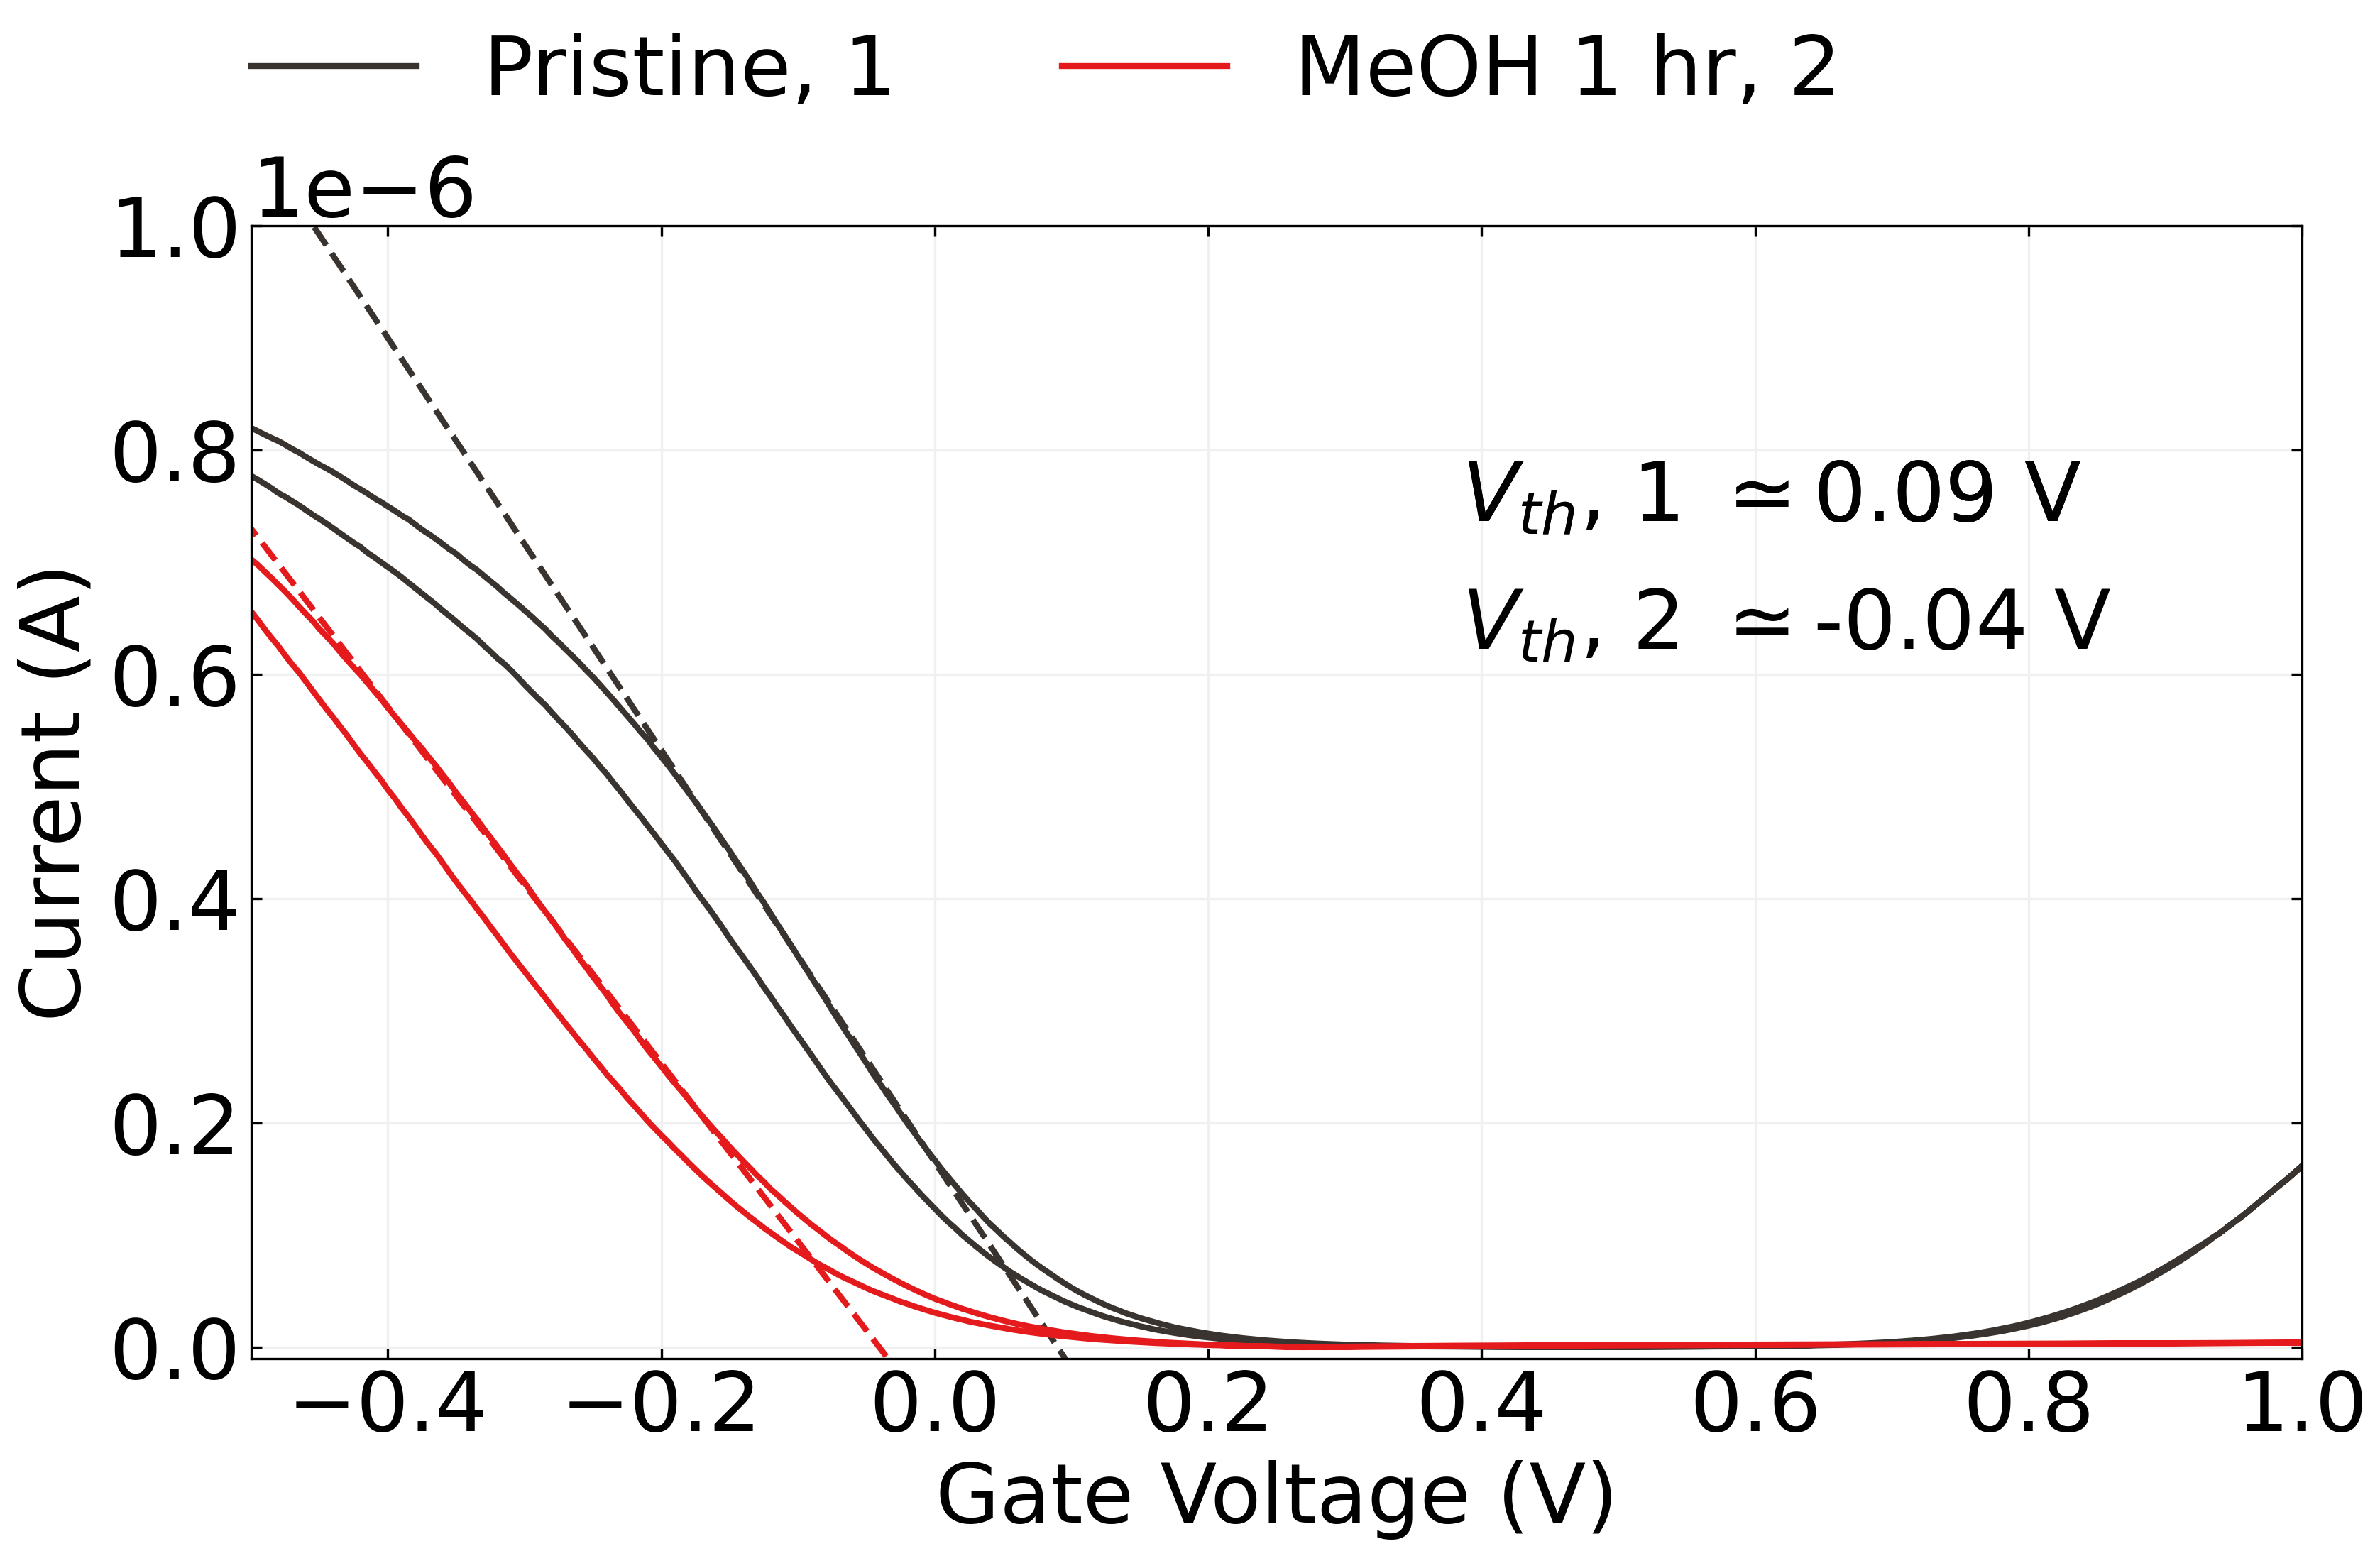
\includegraphics{figures/ch7/Q23D5_ch1_MeOHonly.png}

}

}

\subcaption{\label{fig-meoh-only-tx}}
\end{minipage}%
%
\begin{minipage}[t]{0.50\linewidth}

{\centering 

\raisebox{-\height}{

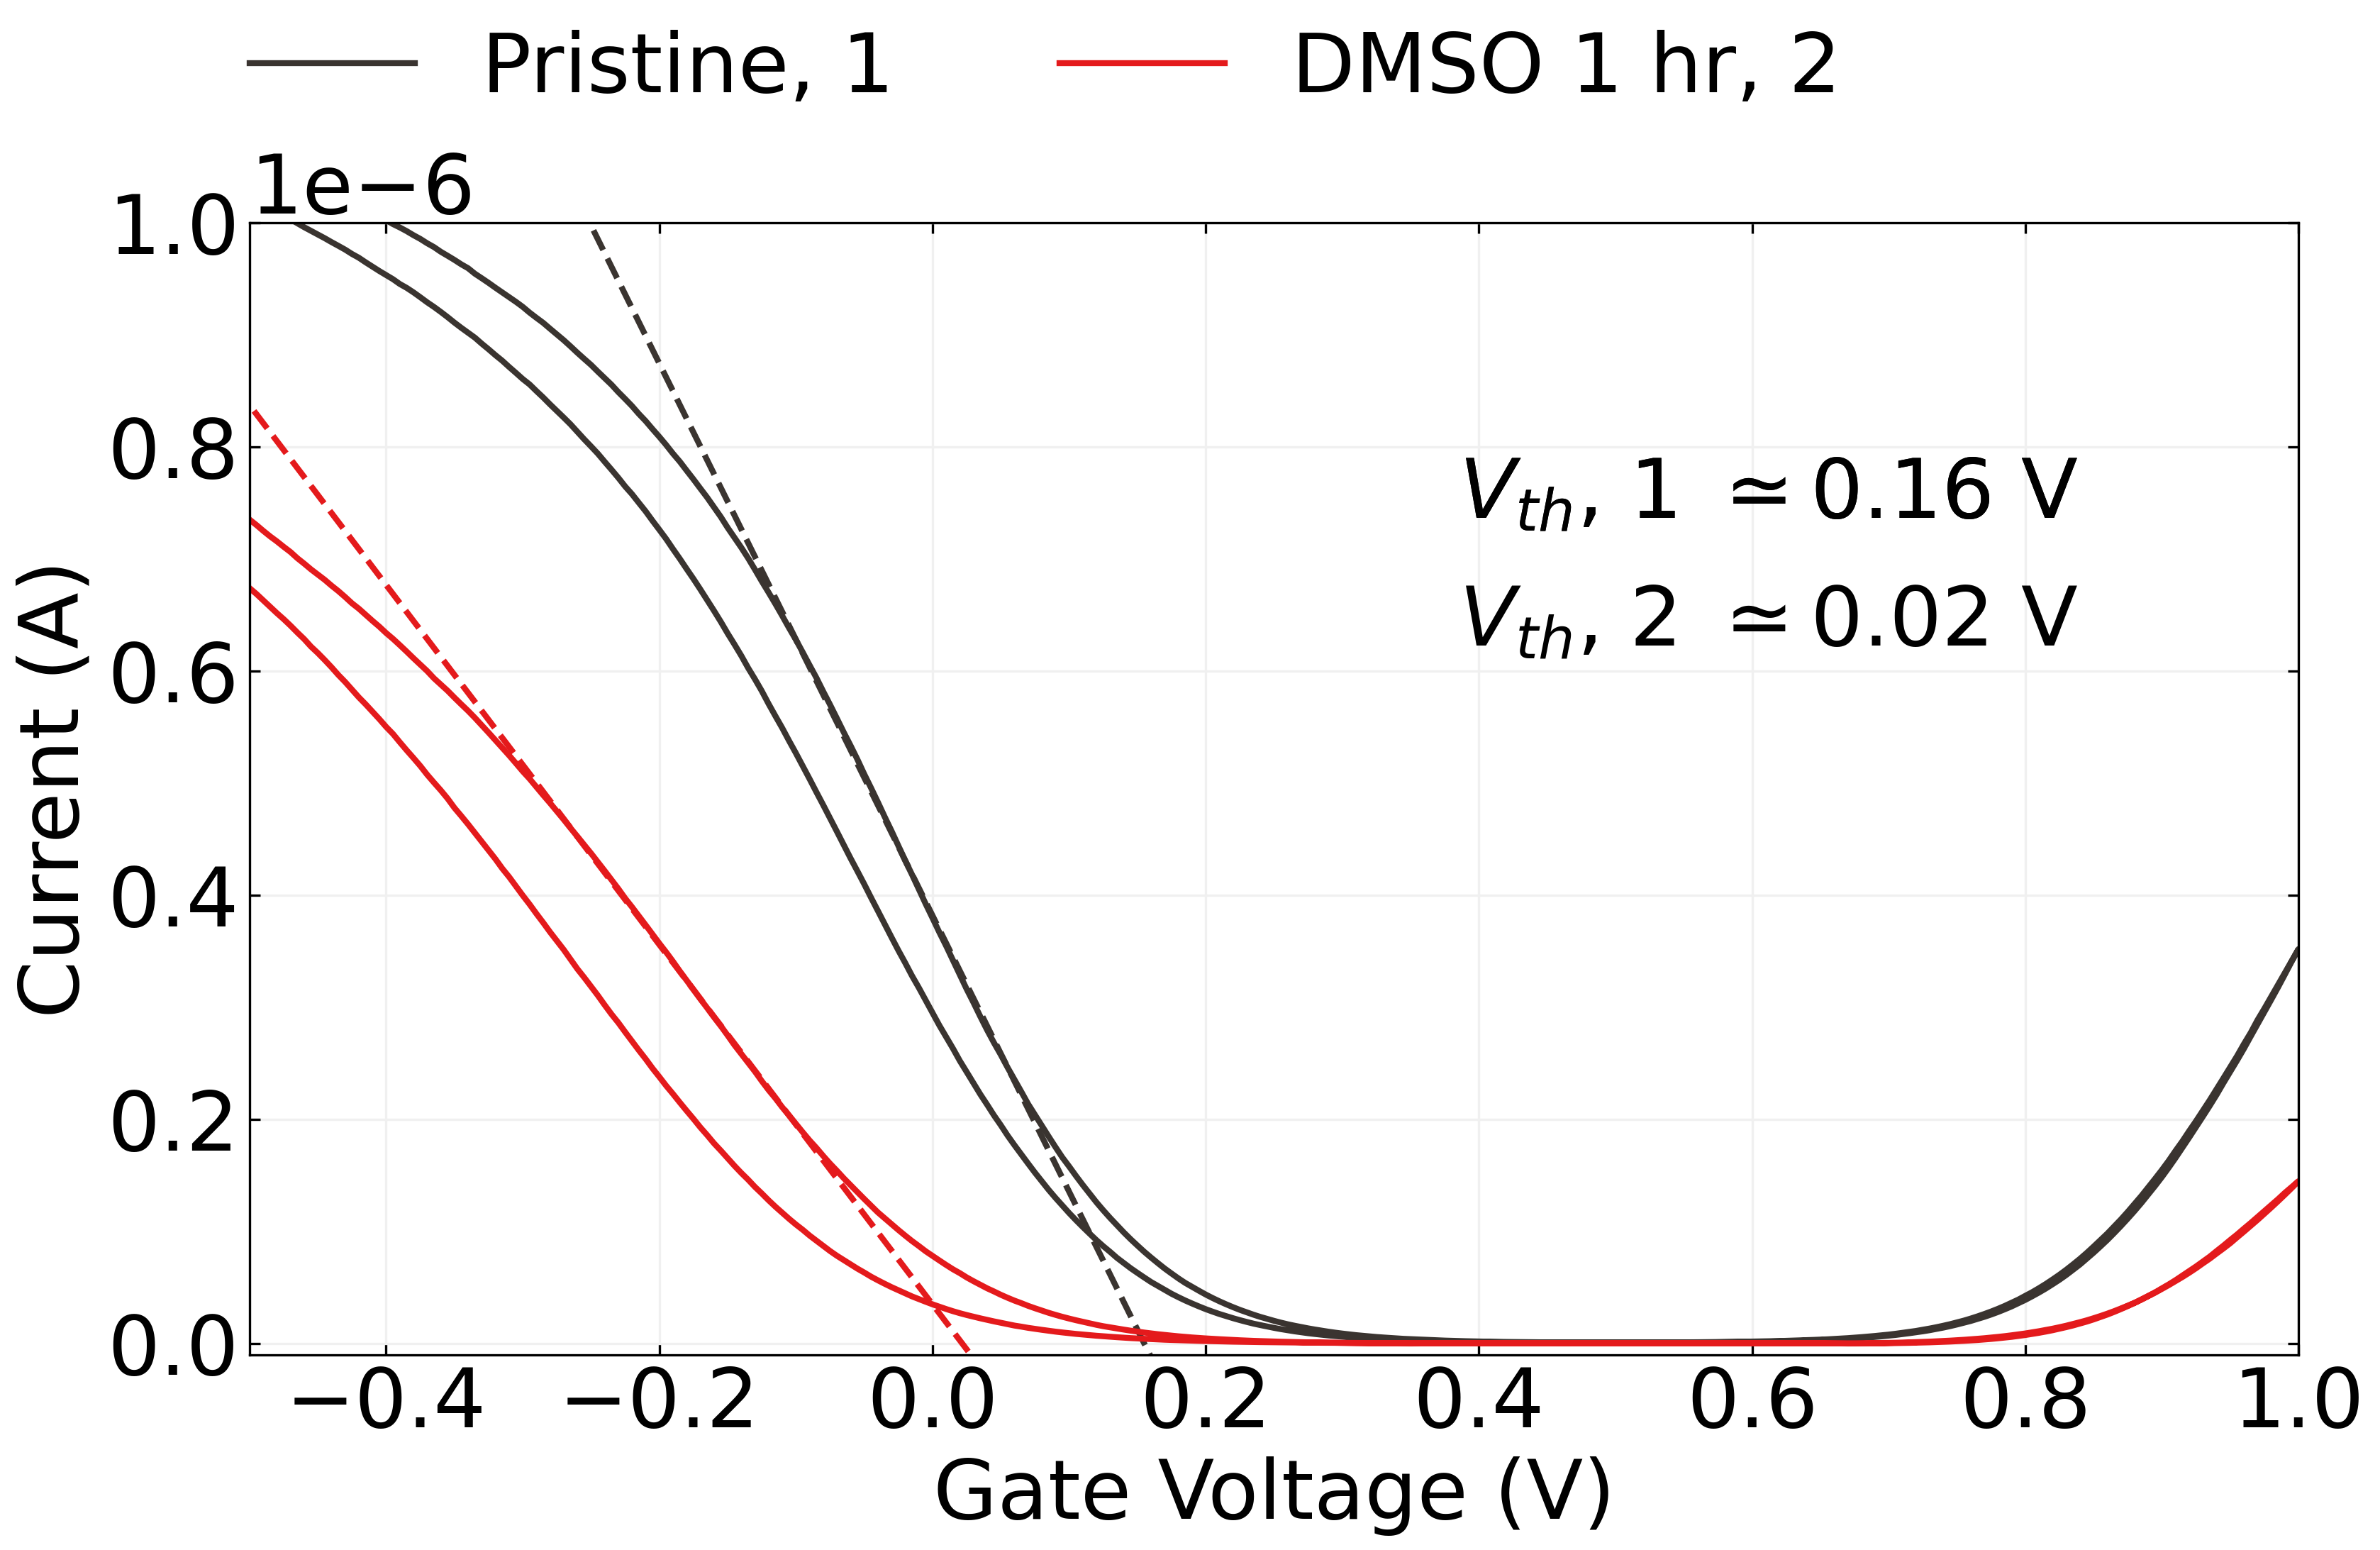
\includegraphics{figures/ch7/Q23D12_ch1_DMSOonly.png}

}

}

\subcaption{\label{fig-dmso-only-tx}}
\end{minipage}%
\newline
\begin{minipage}[t]{0.50\linewidth}

{\centering 

\raisebox{-\height}{

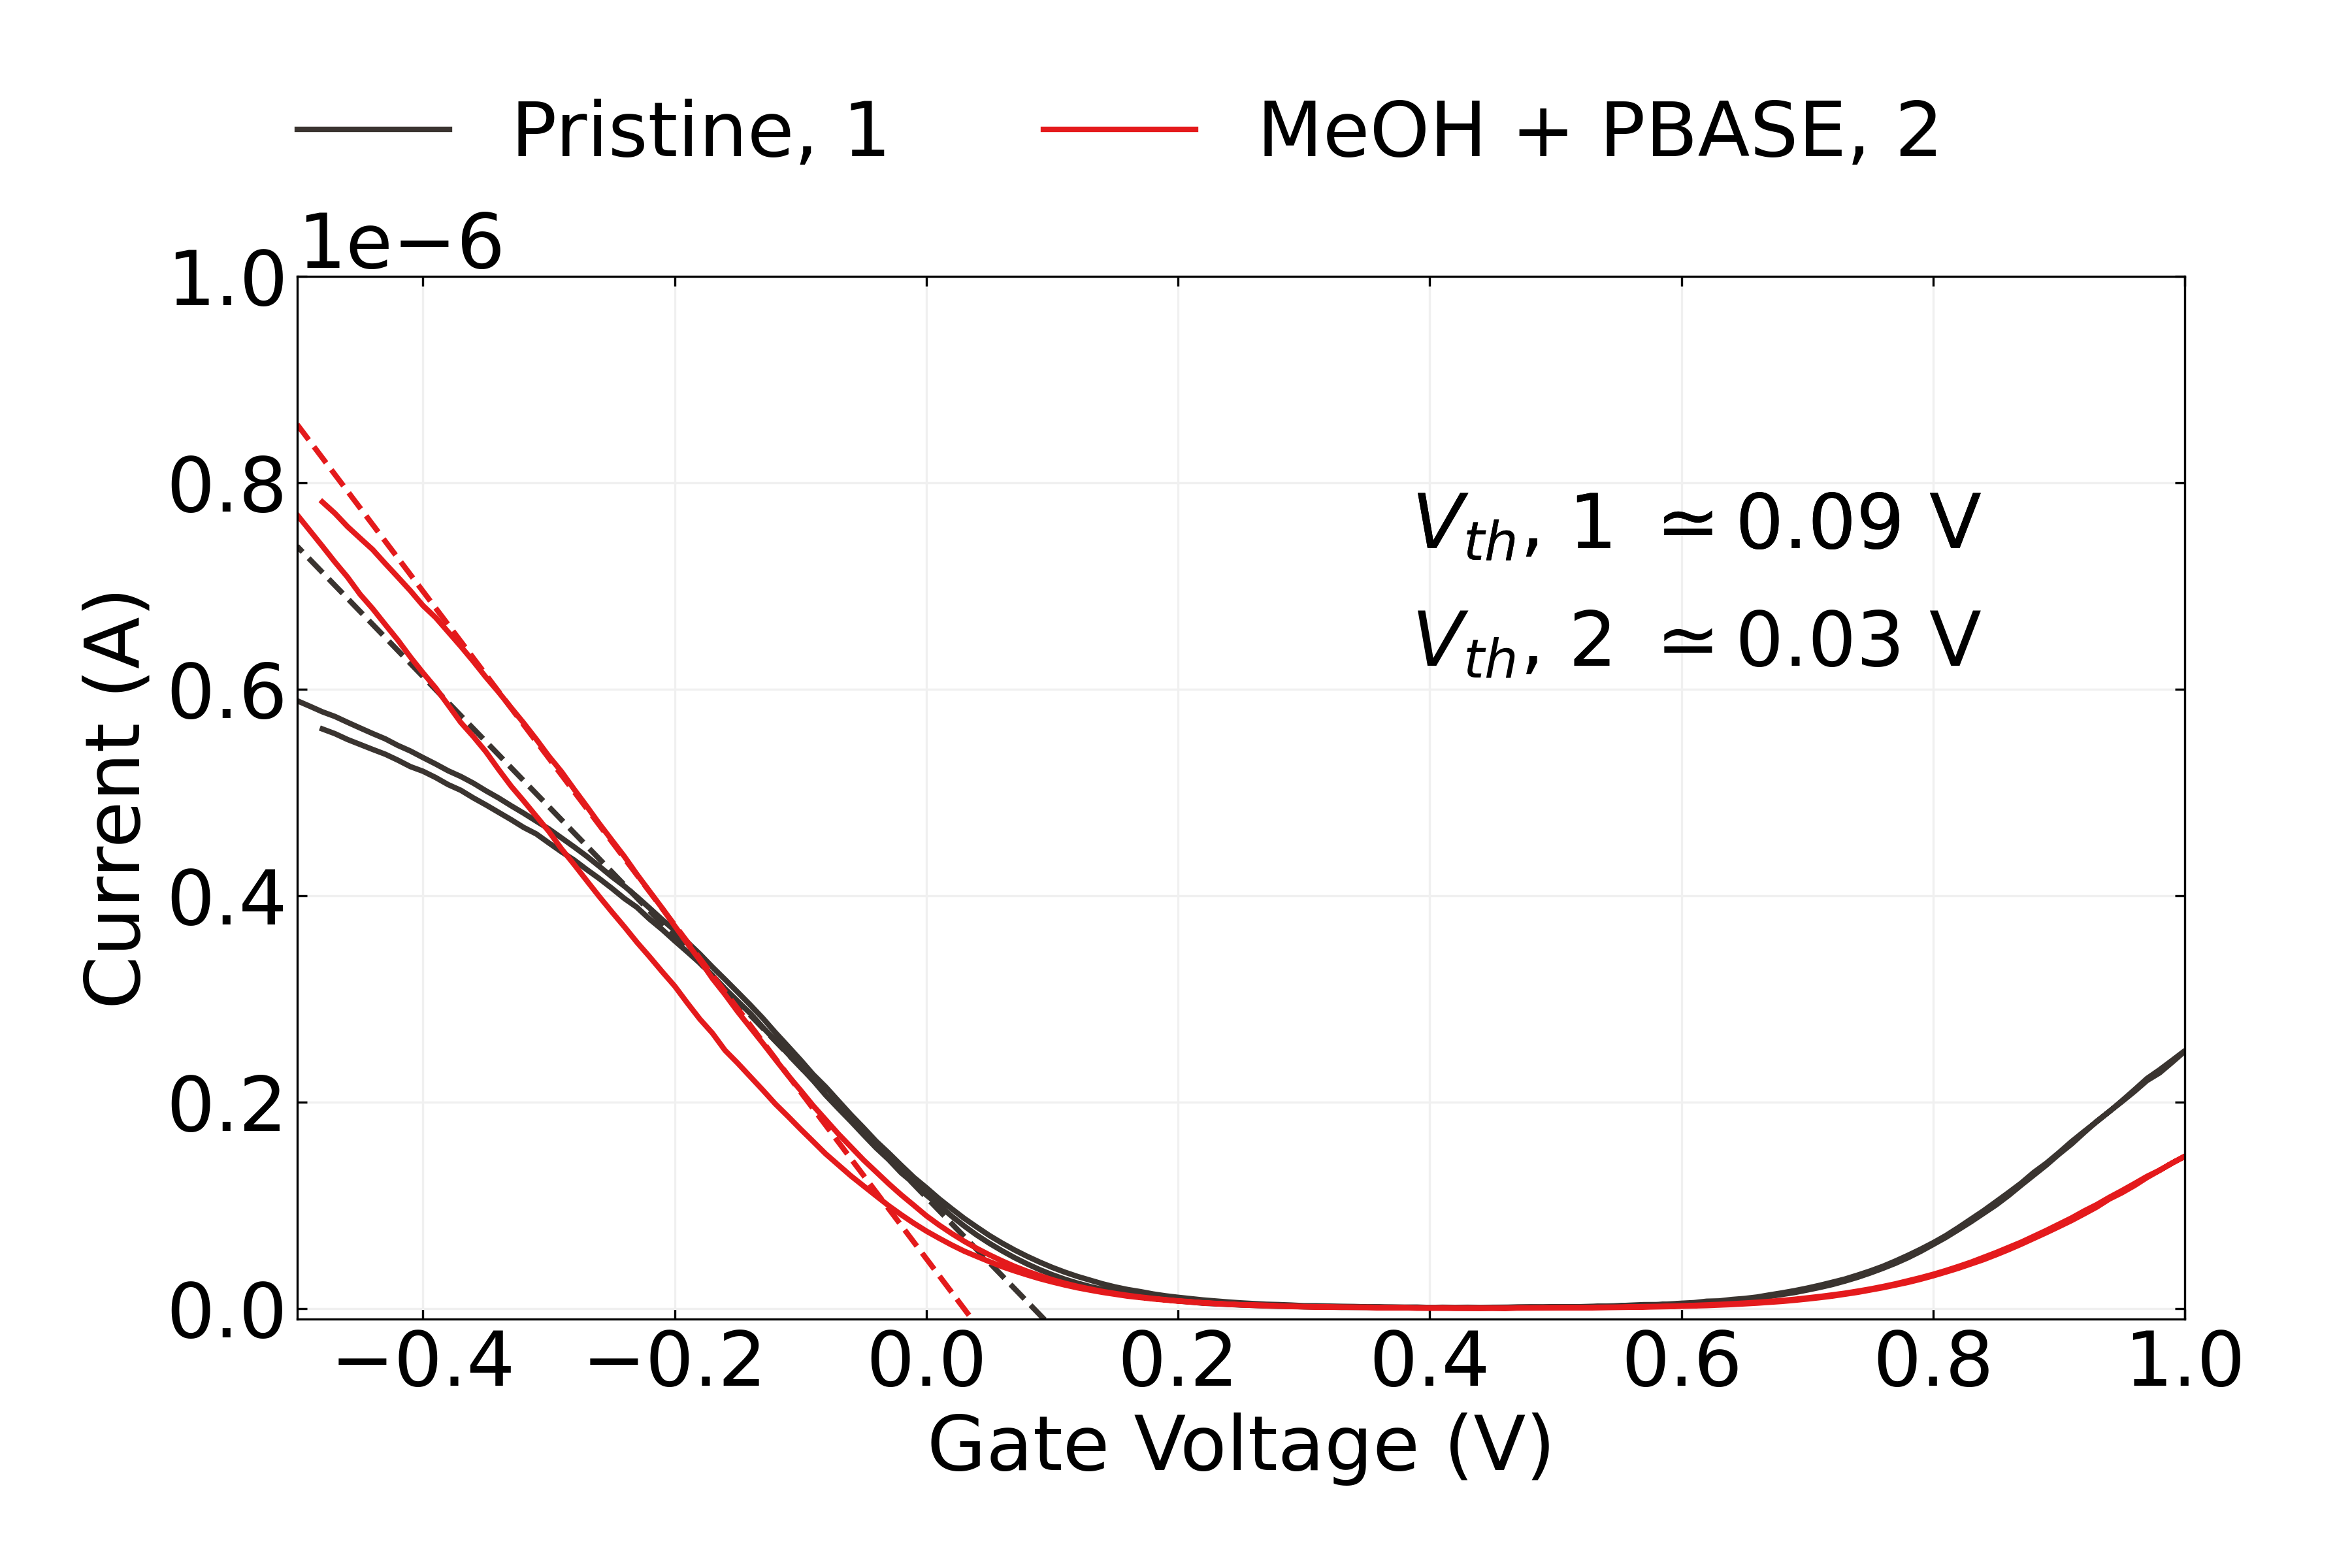
\includegraphics{figures/ch7/Q2C6_ch2_MeOHPBASE.png}

}

}

\subcaption{\label{fig-meoh-pbase-tx}}
\end{minipage}%
%
\begin{minipage}[t]{0.50\linewidth}

{\centering 

\raisebox{-\height}{

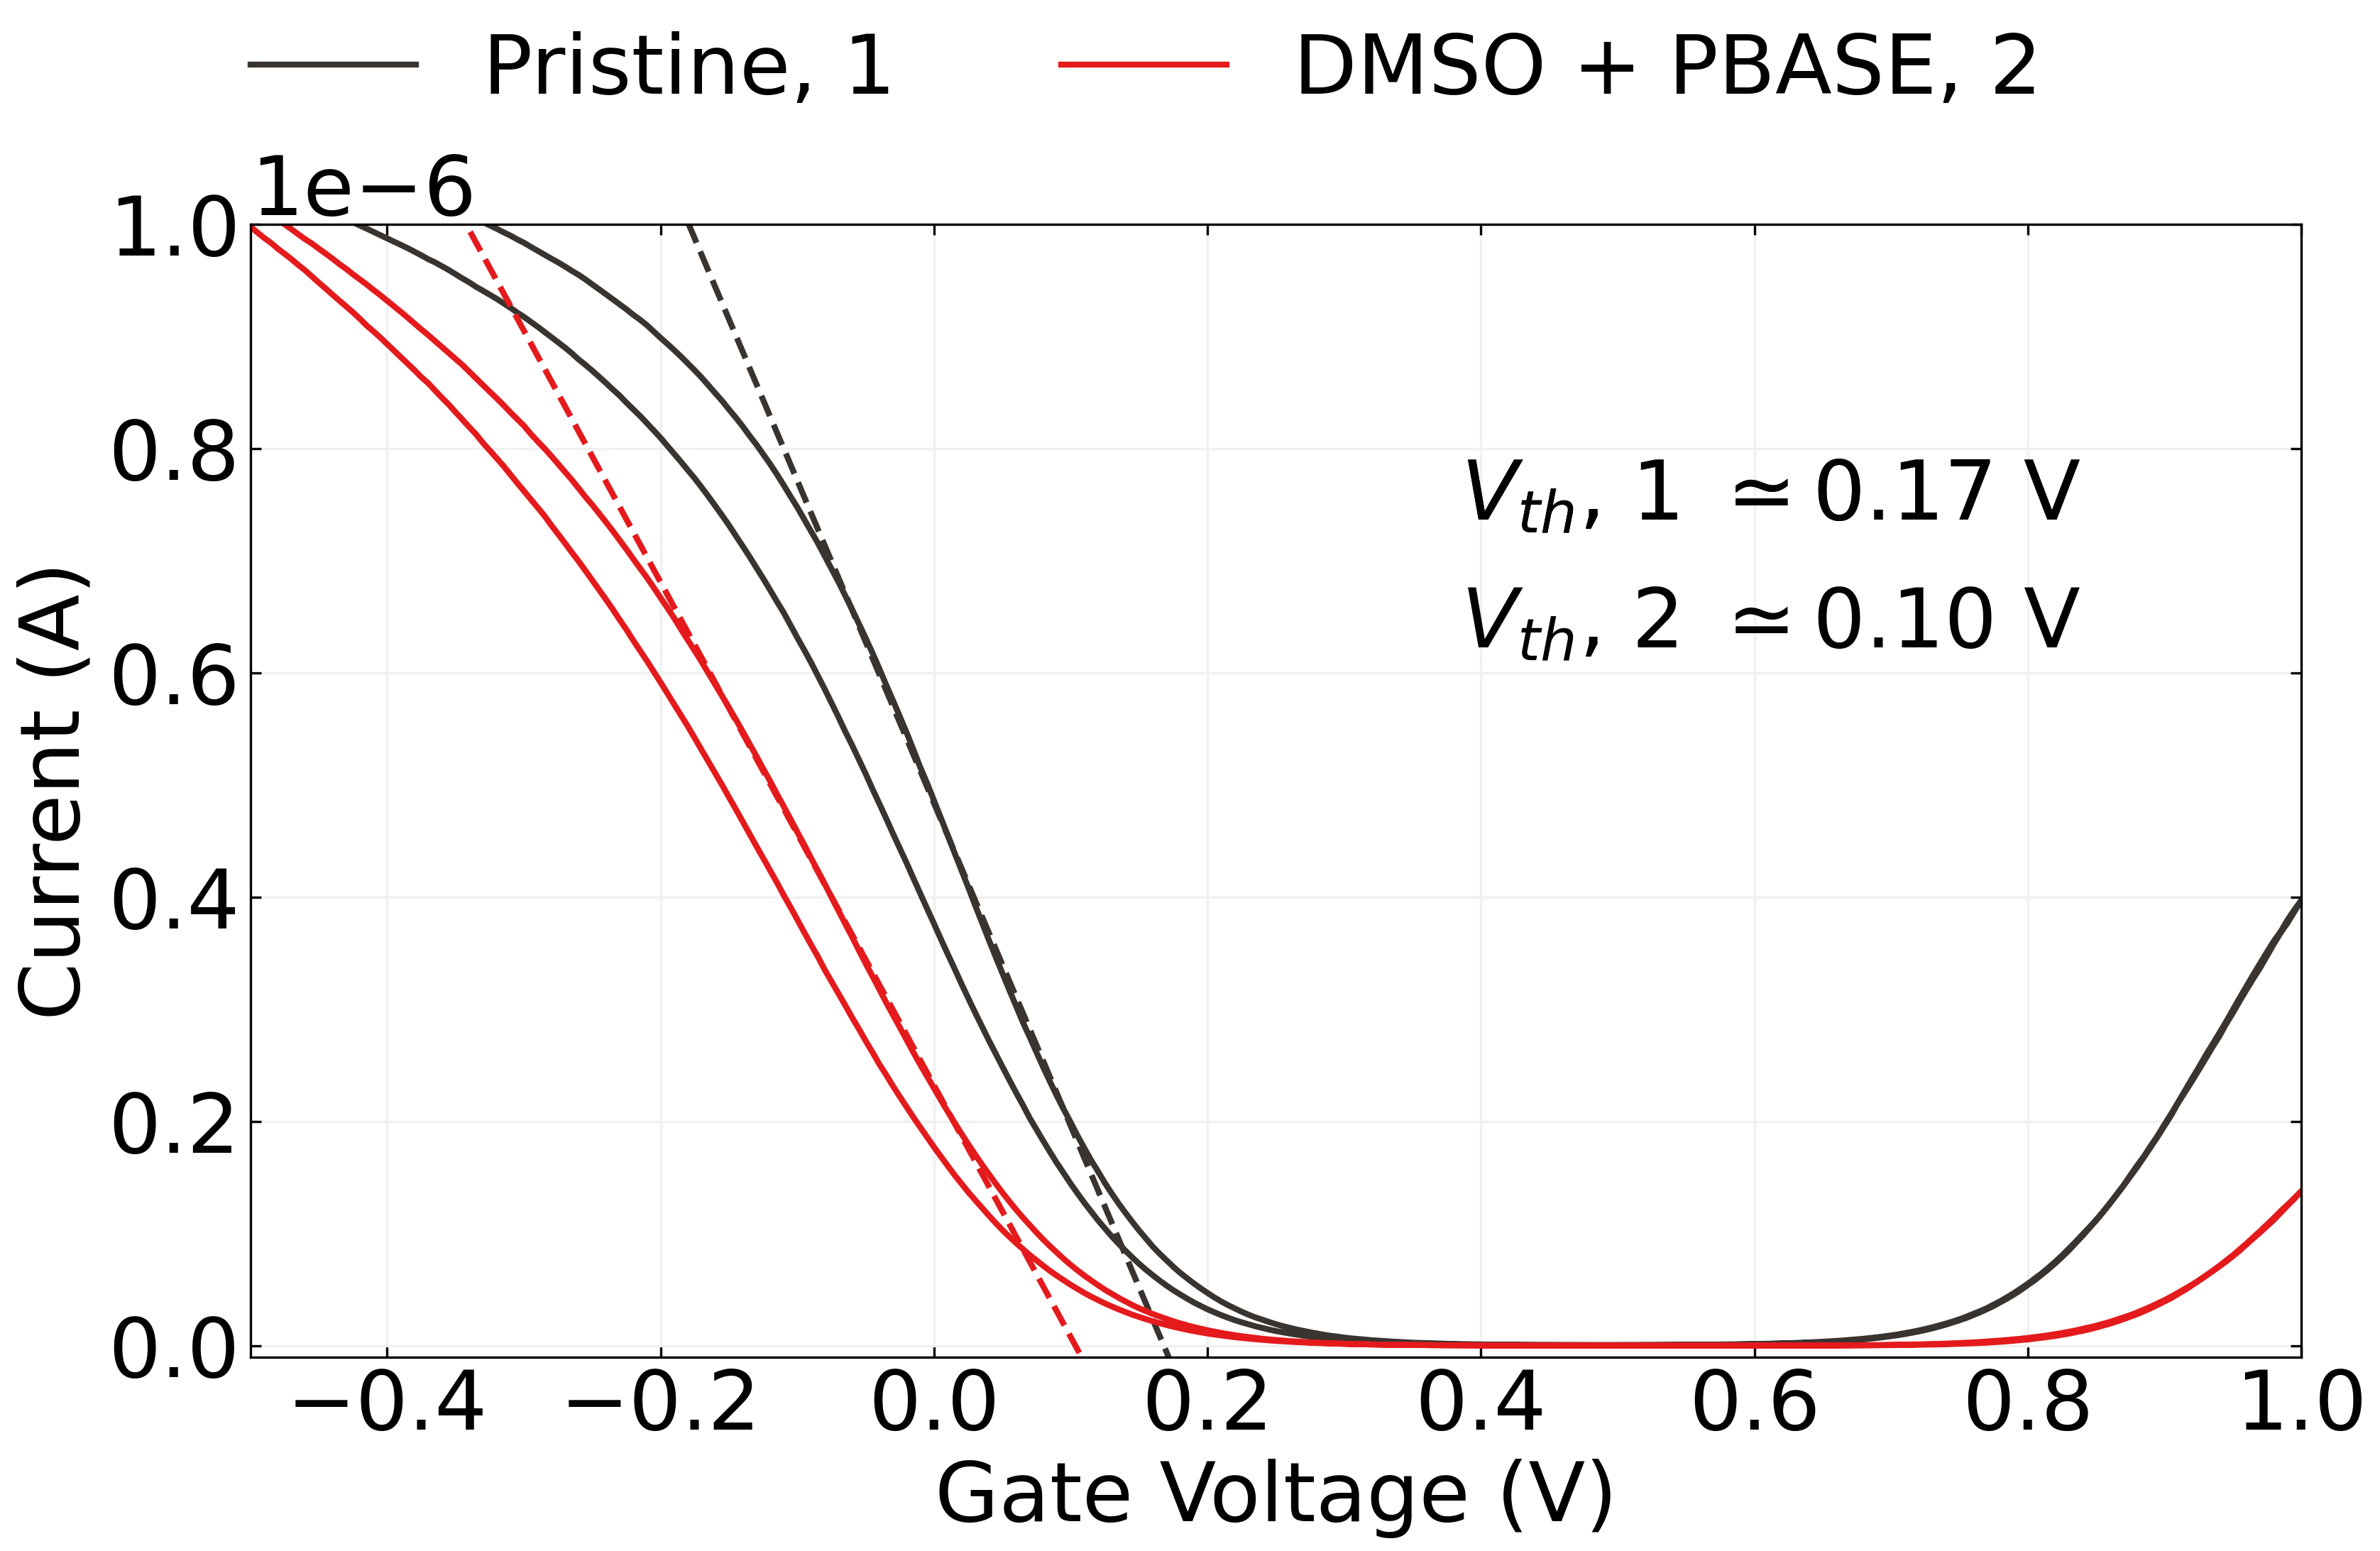
\includegraphics{figures/ch7/Q23D7_ch3_DMSOPBASE.png}

}

}

\subcaption{\label{fig-dmso-pbase-tx}}
\end{minipage}%

\caption{\label{fig-PBASE-vs-solvent-only}The electrical transfer
characteristics of carbon nanotube transistors (\(V_{ds}\) = 100 mV)
before and after being submerged in methanol (a) or dimethyl sulfoxide
(b) for one hour and subsequently rinsed with deionised water. The
change in characteristics of similar transistor channels after being
submerged in these same solvents containing 1 mM PBASE for one hour and
then rinsed are shown in (c) and (d) respectively. Average threshold
voltages for each transfer characteristic curve are also shown (taking
the average of forward and reverse sweep values).}

\end{figure}

The electrical characteristics of the carbon nanotube or graphene
transistor are often used to verify successful functionalisation and
make a statement about the effect of chemical modification on the
channel. However, this verification usually does not account for the
effect of the solvent on the transistor channel.
Figure~\ref{fig-meoh-only-tx} and Figure~\ref{fig-dmso-only-tx} show
that by exposing a steam-deposited carbon nanotube network channel to
solvents commonly used in PBASE functionalisation processes
(Table~\ref{tbl-pbase-functionalisation}), such as methanol (MeOH) or
dimethyl sulfoxide (DMSO), a significant negative shift in channel
threshold voltage occurs even after thorough rinsing with deionised
water. Besteman \emph{et al.} reported observing a similar effect from
prolonged exposure of a single carbon nanotube to dimethylformamide
(DMF) {[}@Besteman2003{]}. It appears that the carbon nanotubes have
adsorped solvent which persists even after device cleaning. From the
shape of the change in the transfer curve, it seems the residual polar
solvent molecules capacitively gate the channel {[}@Artyukhin2006;
@Heller2008{]}.

Furthermore, using the same characterisation process as in this work,
Murugathas \emph{et al.} {[}@Murugathas2019b{]} showed that
\(\pi\)-stacking of PBASE onto a solvent-deposited carbon nanotube
network had little effect on channel threshold voltage, implying the
presence of PBASE had not significantly influenced channel gating
{[}@Murugathas2019b{]}. However, they did observe a slight increase in
channel conductance after PBASE functionalisation. In
Figure~\ref{fig-PBASE-vs-solvent-only}, a slight increase in channel
conductance post-functionalisation is observed for both
Figure~\ref{fig-meoh-pbase-tx} and Figure~\ref{fig-dmso-pbase-tx} when
compared to the solvent-only case in Figure~\ref{fig-meoh-only-tx} and
Figure~\ref{fig-dmso-only-tx}. This result implies that the presence of
PBASE molecules increases channel mobility and therefore conductance
{[}@Heller2008{]}.

Capactive gating results from dense coverage of adsorped molecules on
the carbon nanotube surface which have a low permittivity relative to
the surrounding electrolyte {[}@Heller2008{]}. The relative permittivity
of MeOH and DMSO are \(\sim\) 33 {[}@Mohsen-Nia2010{]} and \(\sim\) 47
{[}@Hunger2010{]} respectively, which are both much lower than the
relative permittivity of phosphate buffer saline, \(\sim\) 80
{[}@Shkodra2021{]}. From Figure~\ref{fig-meoh-only-tx} and
Figure~\ref{fig-dmso-only-tx}, the threshold shift values found
resulting from exposure to each solvent, taking the average of forward
and reverse sweep values from a single device, were \(\Delta\)V =
\(-0.15 \pm 0.02\) V and \(\Delta\)V = \(-0.15 \pm 0.01\) V for MeOH and
DMSO respectively. The average threshold shift value for a second device
exposed to MeOH was \(\Delta\)V = \(-0.16 \pm 0.02\) V, indicating that
this threshold shift result is reproducible. The threshold voltage
shifts in Figure~\ref{fig-meoh-pbase-tx} and
Figure~\ref{fig-dmso-pbase-tx} from the pristine are small compared with
the devices exposed to solvent only - this is likely due to the effect
of increased conductance from the PBASE competing with the gating effect
from the residual solvent.

The absorption of organic solvent by the carbon nanotube network has
unknown but potentially negative implications for biosensor
functionalisation. Use of organic solvents in functionalisation can also
attack the encapsulation layer of devices, promoting gate current
leakage. In light of these issues, recent work has begun to explore
alternative aqueous-based methods for functionalisation of biosensors
{[}@Khan2021{]}. The discussion here also illustrates the importance of
considering each substance used when electrical characterising a device
to verify if functionalisation has worked. The qualitative presence of a
change in characteristics (or lack of one) over the full process is not
sufficient to make conclusive remarks regarding successful
functionalisation. A full set of electrical control measurements are
required for an understanding of electronic changes occuring during the
functionalisation process, in the manner of Besteman \emph{et al.}
{[}@Besteman2003{]}.

\newpage
\KOMAoptions{paper=landscape,pagesize}

\hfill\break
\hfill\break

\hypertarget{tbl-pba-functionalisation}{}
\begin{longtable}[]{@{}llllllll@{}}
\caption{\label{tbl-pba-functionalisation}Comparison of 1-pyrenebutyric
acid (PBA) functionalisation processes used for immobilisation of
proteins, enzymes and aptamers onto carbon nanotubes and graphene.
1-ethyl-3-(3-dimethylaminopropyl) carbodiimide hydrochloride (EDC) and
NHS were co-mingled in buffer/electrolyte solution or DI water in each
process - some papers used N-hydroxysulfosuccinimide instead of
N-hydroxysuccinimide, and both compounds are abbreviated as NHS in this
table for simplicity. Device exposure times to each solution are shown
next to the solution concentration. Blank entries indicate there was no
mention of the parameter in a particular paper. \(^†\)PEG or PEG pyrene
were used to reduce non-specific binding. \(^{††}\)Several pyrene-based
linkers were compared and PBA gave an optimal functionalisation
result.}\tabularnewline
\toprule\noalign{}
Solvent & Channel & PBA (mM) & Time (hr) & EDC (mM) & NHS (mM) & Time
(min) & References \\
\midrule\noalign{}
\endfirsthead
\toprule\noalign{}
Solvent & Channel & PBA (mM) & Time (hr) & EDC (mM) & NHS (mM) & Time
(min) & References \\
\midrule\noalign{}
\endhead
\bottomrule\noalign{}
\endlastfoot
DMF & Graphene & 0.6 & 1 & - & - & 120 & Gao, 2016\(^†\).
\cite{Gao2016} \\
& & 5 & 2 & 2 & 5 & 30 & Mishyn, 2022. \cite{Mishyn2022} \\
& CNT & 100 & 3 & 200 & - & 30 & Min, 2012. \cite{Min2012} \\
& Graphene, CNT & 7.6 & 2 & 8 & 20 & 120 & Xu, 2014. \cite{Xu2014} \\
DI water & CNT & - & - & 32 & 12 & Overnight & Pacios, 2012\(^†\).
\cite{Pacios2012} \\
Ethanol & CNT & 1 & 1 & 100 & 100 & 20 & Filipiak, 2018\(^†\).
\cite{Filipiak2018} \\
Acetonitrile & Graphene & 1 & 1 & 400 & 100 & 60 & Tong, 2020\(^{††}\).
\cite{Tong2020} \\
Borax & CNT & 2 & 24 & 2.5 & - & 1080 & Liu, 2011\(^†\).
\cite{Liu2011} \\
DMSO & Graphene & 5 & 1 & 50 & 50 & 90 & Fenzl, 2017.
\cite{Fenzl2017} \\
\end{longtable}

\newpage
\KOMAoptions{paper=portrait,pagesize}

\hypertarget{sec-PBA}{%
\subsection{Attachment of 1-Pyrenebutyric Acid}\label{sec-PBA}}

\hypertarget{comparing-attachment-methods-1}{%
\subsubsection{Comparing Attachment
Methods}\label{comparing-attachment-methods-1}}

Another linker molecule that can be used to attach receptor molecules to
a carbon nanotube or graphene channel is 1-pyrenebutyric acid (PBA or
PyBA). As with PBASE, the pyrene group of PBA has a \(\pi\) interaction
with the carbon rings of the channel surface. It is possible to react
PBA with 1-ethyl-3-(3-dimethylaminopropyl) carbodiimide hydrochloride
(EDC or EDAC) to form an \emph{O}-acylisourea intermediate, which can
then react with an amine group on a biomolecule and form an amide bond
{[}@Sehgal1994; @Hermanson2013-4{]}. The water solubility of EDC means
that, unlike PBASE, it is possible to functionalise with EDC dissolved
in water rather than in an organic solvent. However, like PBASE, EDC and
the \emph{O}-acylisourea intermediate are prone to hydrolysis,
especially in acidic conditions. Therefore, like PBASE, it should be
stored at −20°C, and warmed to room temperature to prevent condensation
build-up, since exposure to condensation will hydrolyse the reagent
{[}@Hermanson2013-4{]}. Furthermore, by adding N-Hydroxysuccinimide
(NHS) or N-hydroxysulfosuccinimide (sulfo-NHS) to the reaction vessel,
PBASE is formed as an active intermediate, which is less prone to
hydrolysis and increases the PBA/EDC reaction yield {[}@Sehgal1994;
@Hermanson2013-4; @Hermanson2013-14{]}.

A full comparison of functionalisation procedures used for linking
carbon nanotube and graphene devices to aptamers and proteins with PBA
is given in Table~\ref{tbl-pba-functionalisation}. To the best of my
knowledge, this table is as complete a summary as possible of
1-pyrenebutyric acid functionalisation processes for carbon nanotube and
graphene field-effect transistor biochemical sensors. By comparing
Table~\ref{tbl-pbase-functionalisation} and
Table~\ref{tbl-pba-functionalisation}, it is clear that PBASE is more
widely used for non-covalent functionalisation than PBA/EDC. As was the
case for PBASE, there are a wide range of process variables used for the
functionalisation process, with little justification used for variables
chosen. Also notable is the frequent use of polyethylene glycol (PEG) or
pyrene-PEG for prevention of non-specific binding (NSB). Non-specific
binding is discussed further in \textbf{?@sec-non-specific-binding}.
Despite being less widely used, Mishyn \emph{et al.} {[}@Mishyn2022{]}
state a preference for the use of PBA/EDC over PBASE, as they found it
was less prone to hydrolysis and gave a larger reaction yield when
binding ferrocene to graphene. A potential downside of using PBA/EDC for
protein immobilisation is that EDC has numerous ways of interacting with
proteins, and not all of these are necessarily desirable; furthermore,
the addition of NHS may also cause other issues, such as precipitation
of the reaction compound {[}@Hermanson2013-4{]}. The greater range of
process variables involved in the functionalisation also adds to the
complexity of reproducing past results.

\hypertarget{raman-spectroscopy}{%
\subsubsection{Raman Spectroscopy}\label{raman-spectroscopy}}

\begin{figure}

{\centering 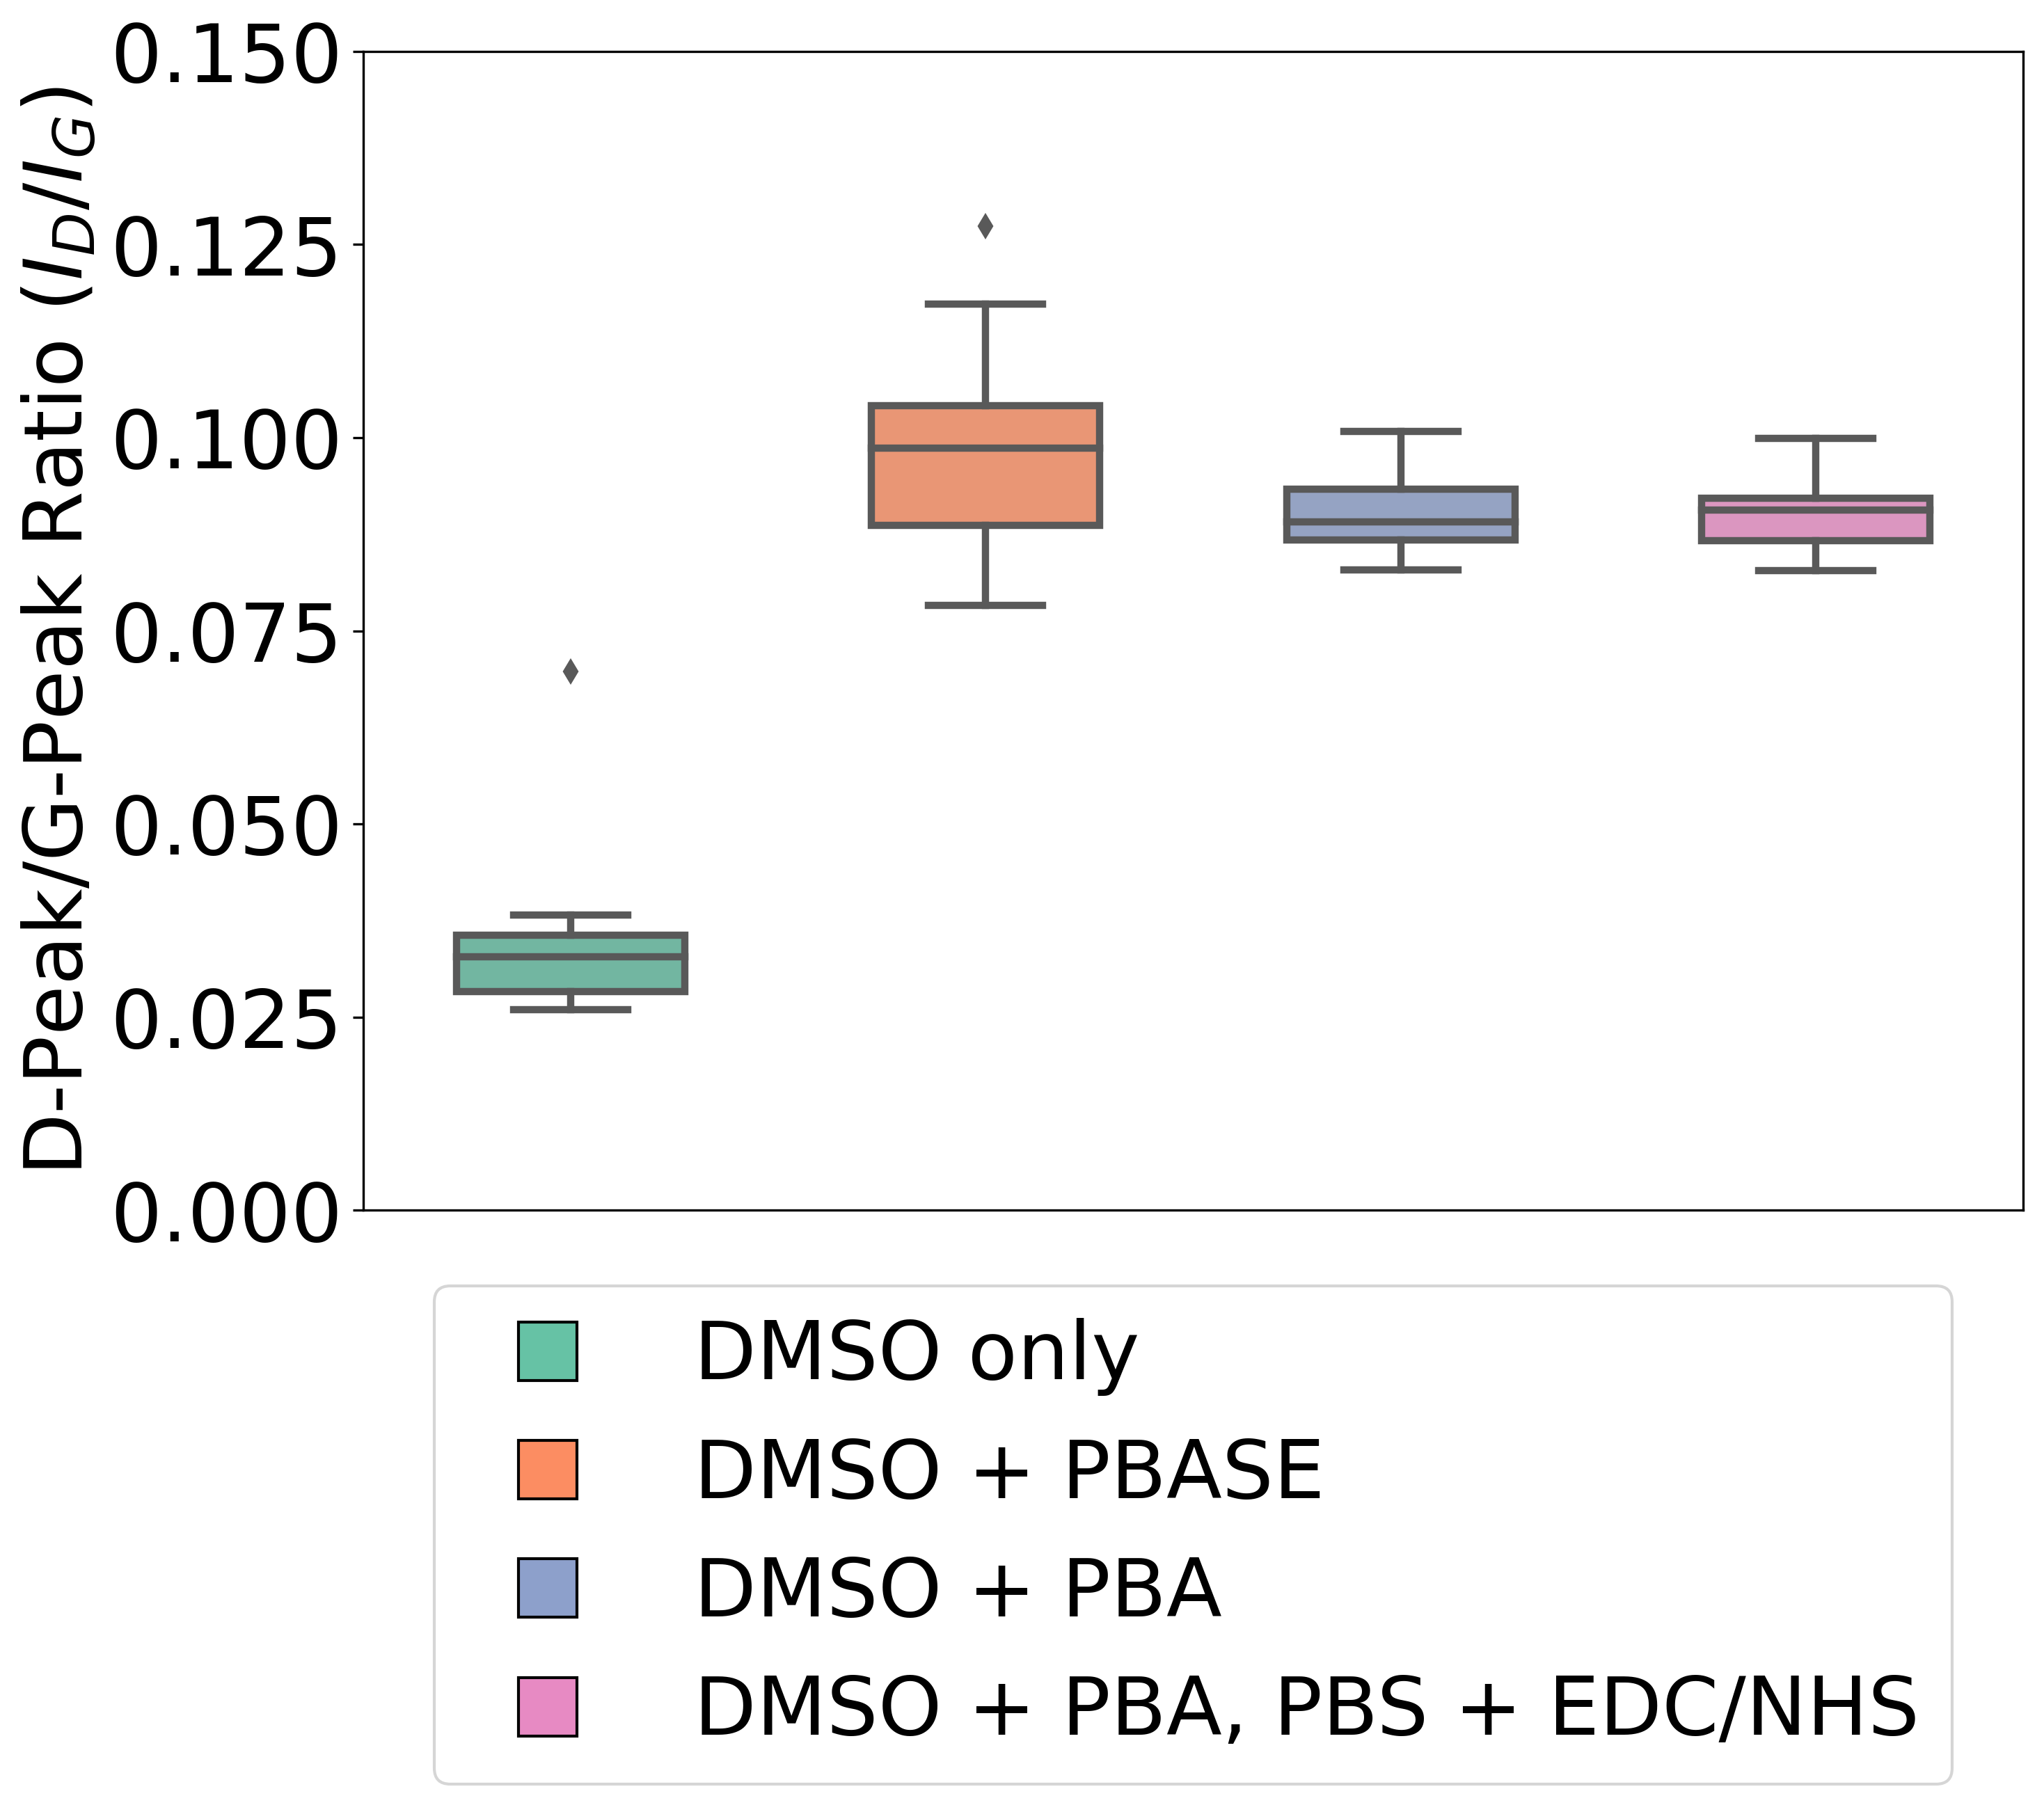
\includegraphics[width=0.5\textwidth,height=\textheight]{figures/ch7/comparison_raman.png}

}

\caption{\label{fig-linker-raman}This box plot shows the distribution of
D-band peak to G\(^+\)-band peak ratio, I\(_D\)/I\(_G\), across nine
locations for a selection of chemically-modified carbon nanotube films.
The D-band and G-band intensities for all samples were first normalised
to the intensity peak corresponding to the silicon dioxide substrate.}

\end{figure}

Raman spectroscopy was used to verify the attachment of PBA to a carbon
nanotube network film with a silicon dioxide substrate in the manner
outlined in \textbf{?@sec-raman-characterisation}. As highly-bundled
devices were found to have less defects present prior to modification,
as discussed in \textbf{?@sec-pristine-raman}, solvent-deposited films
were used for the verification of pyrene attachment to prevent the
initial presence of defects influencing the analysis. Droplets of DMSO
solution were placed on three (solvent-deposited) carbon nanotube films
taken from the same wafer. The DMSO solution on one film contained 5 mM
PBA, the solution on another film contained 5 mM PBASE, and the DMSO on
the final film contained no linker molecule. After incubation for 1
hour, films were rinsed for 15 s with DMSO, then for 15 s with IPA to
remove excess DMSO while avoiding hydrolysis of the PBASE. After the
first set of Raman spectra was taken, the film initially exposed to PBA
was further exposed to a solution of 20 mM EDC and 40 mM NHS in 1XPBS
electrolyte for 30 minutes, and a second set of Raman spectra was taken
for this film. As in \textbf{?@sec-pristine-raman}, two spectra taken at
each position were processed according to \textbf{?@sec-raman-analysis},
and the silicon dioxide reference peak measured in the wavenumber range
100 cm\(^{-1}\) \(-\) 650 cm\(^{-1}\) was used to normalise the D-band
and G-band peaks from the wavenumber range 1300 cm\(^{-1}\) \(-\) 1650
cm\(^{-1}\). The ratio between the average intensity of the D-peak and
the G\(^+\)-peak at each position was calculated, and the distribution
of ratio values corresponding to each modified film is shown in
Figure~\ref{fig-linker-raman}.

\begin{figure}

\begin{minipage}[t]{0.50\linewidth}

{\centering 

\raisebox{-\height}{

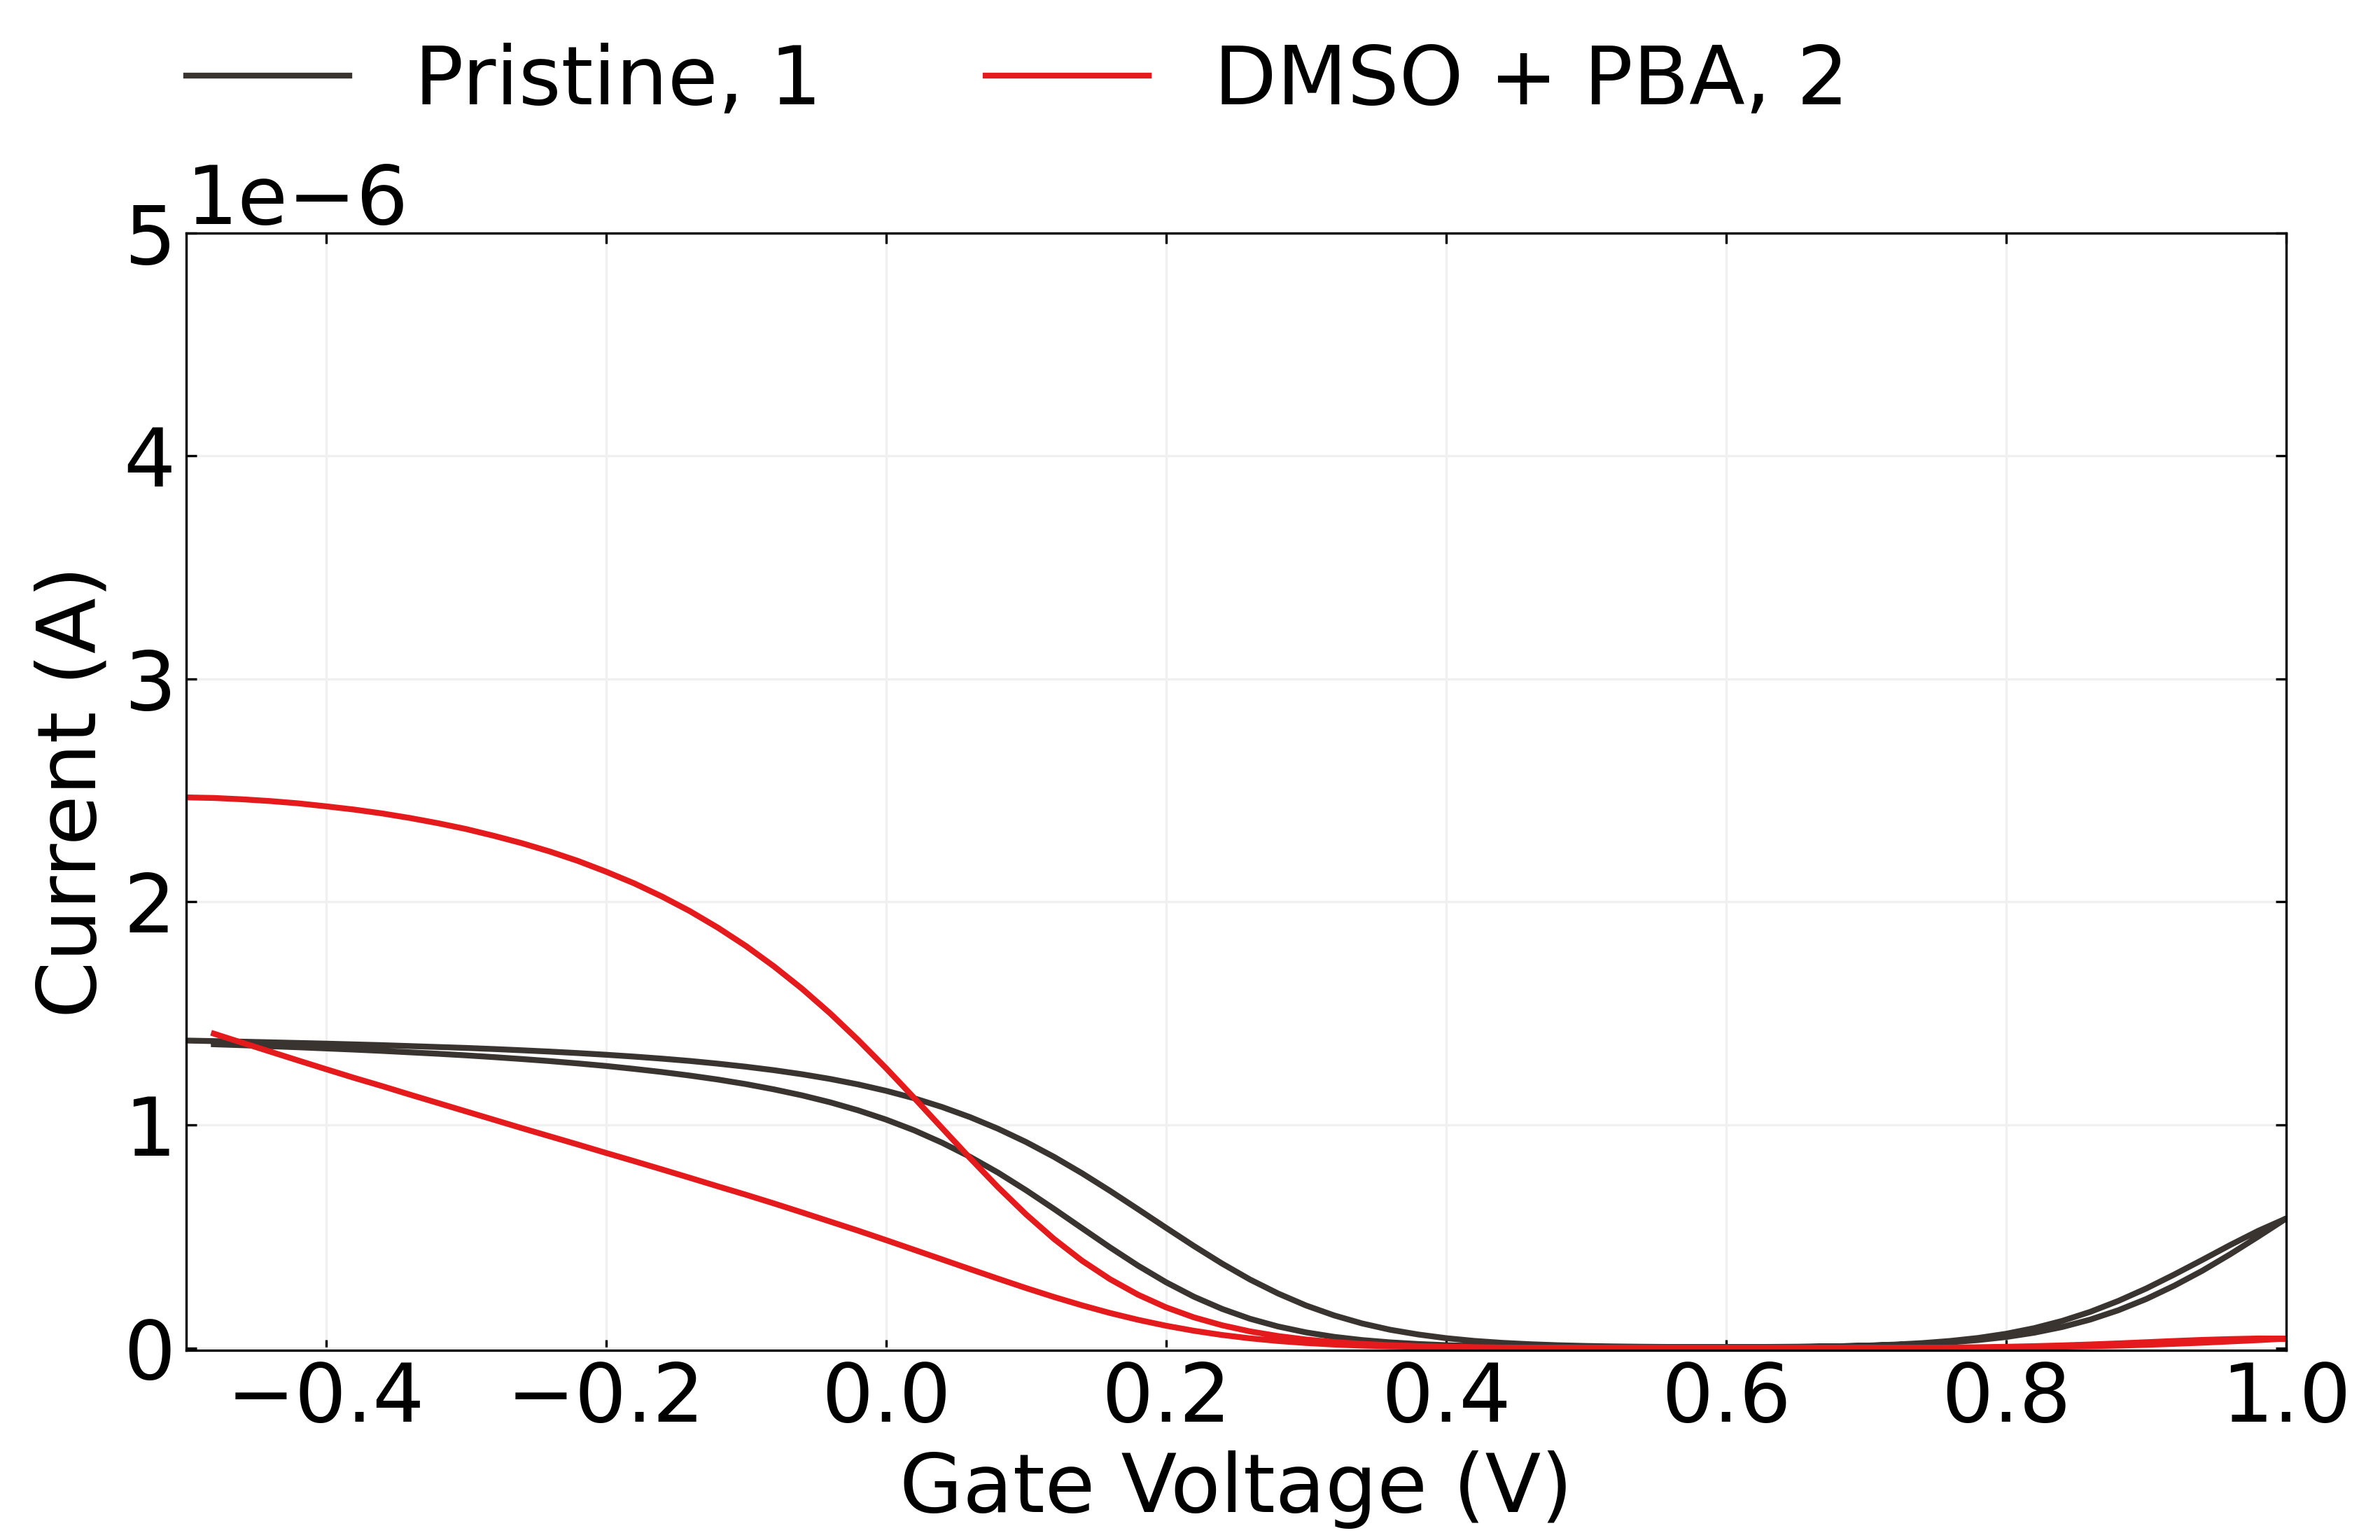
\includegraphics{figures/ch7/NTQ24C10_ch3_comparison_1.png}

}

}

\subcaption{\label{fig-pba-threshold-shift}}
\end{minipage}%
%
\begin{minipage}[t]{0.50\linewidth}

{\centering 

\raisebox{-\height}{

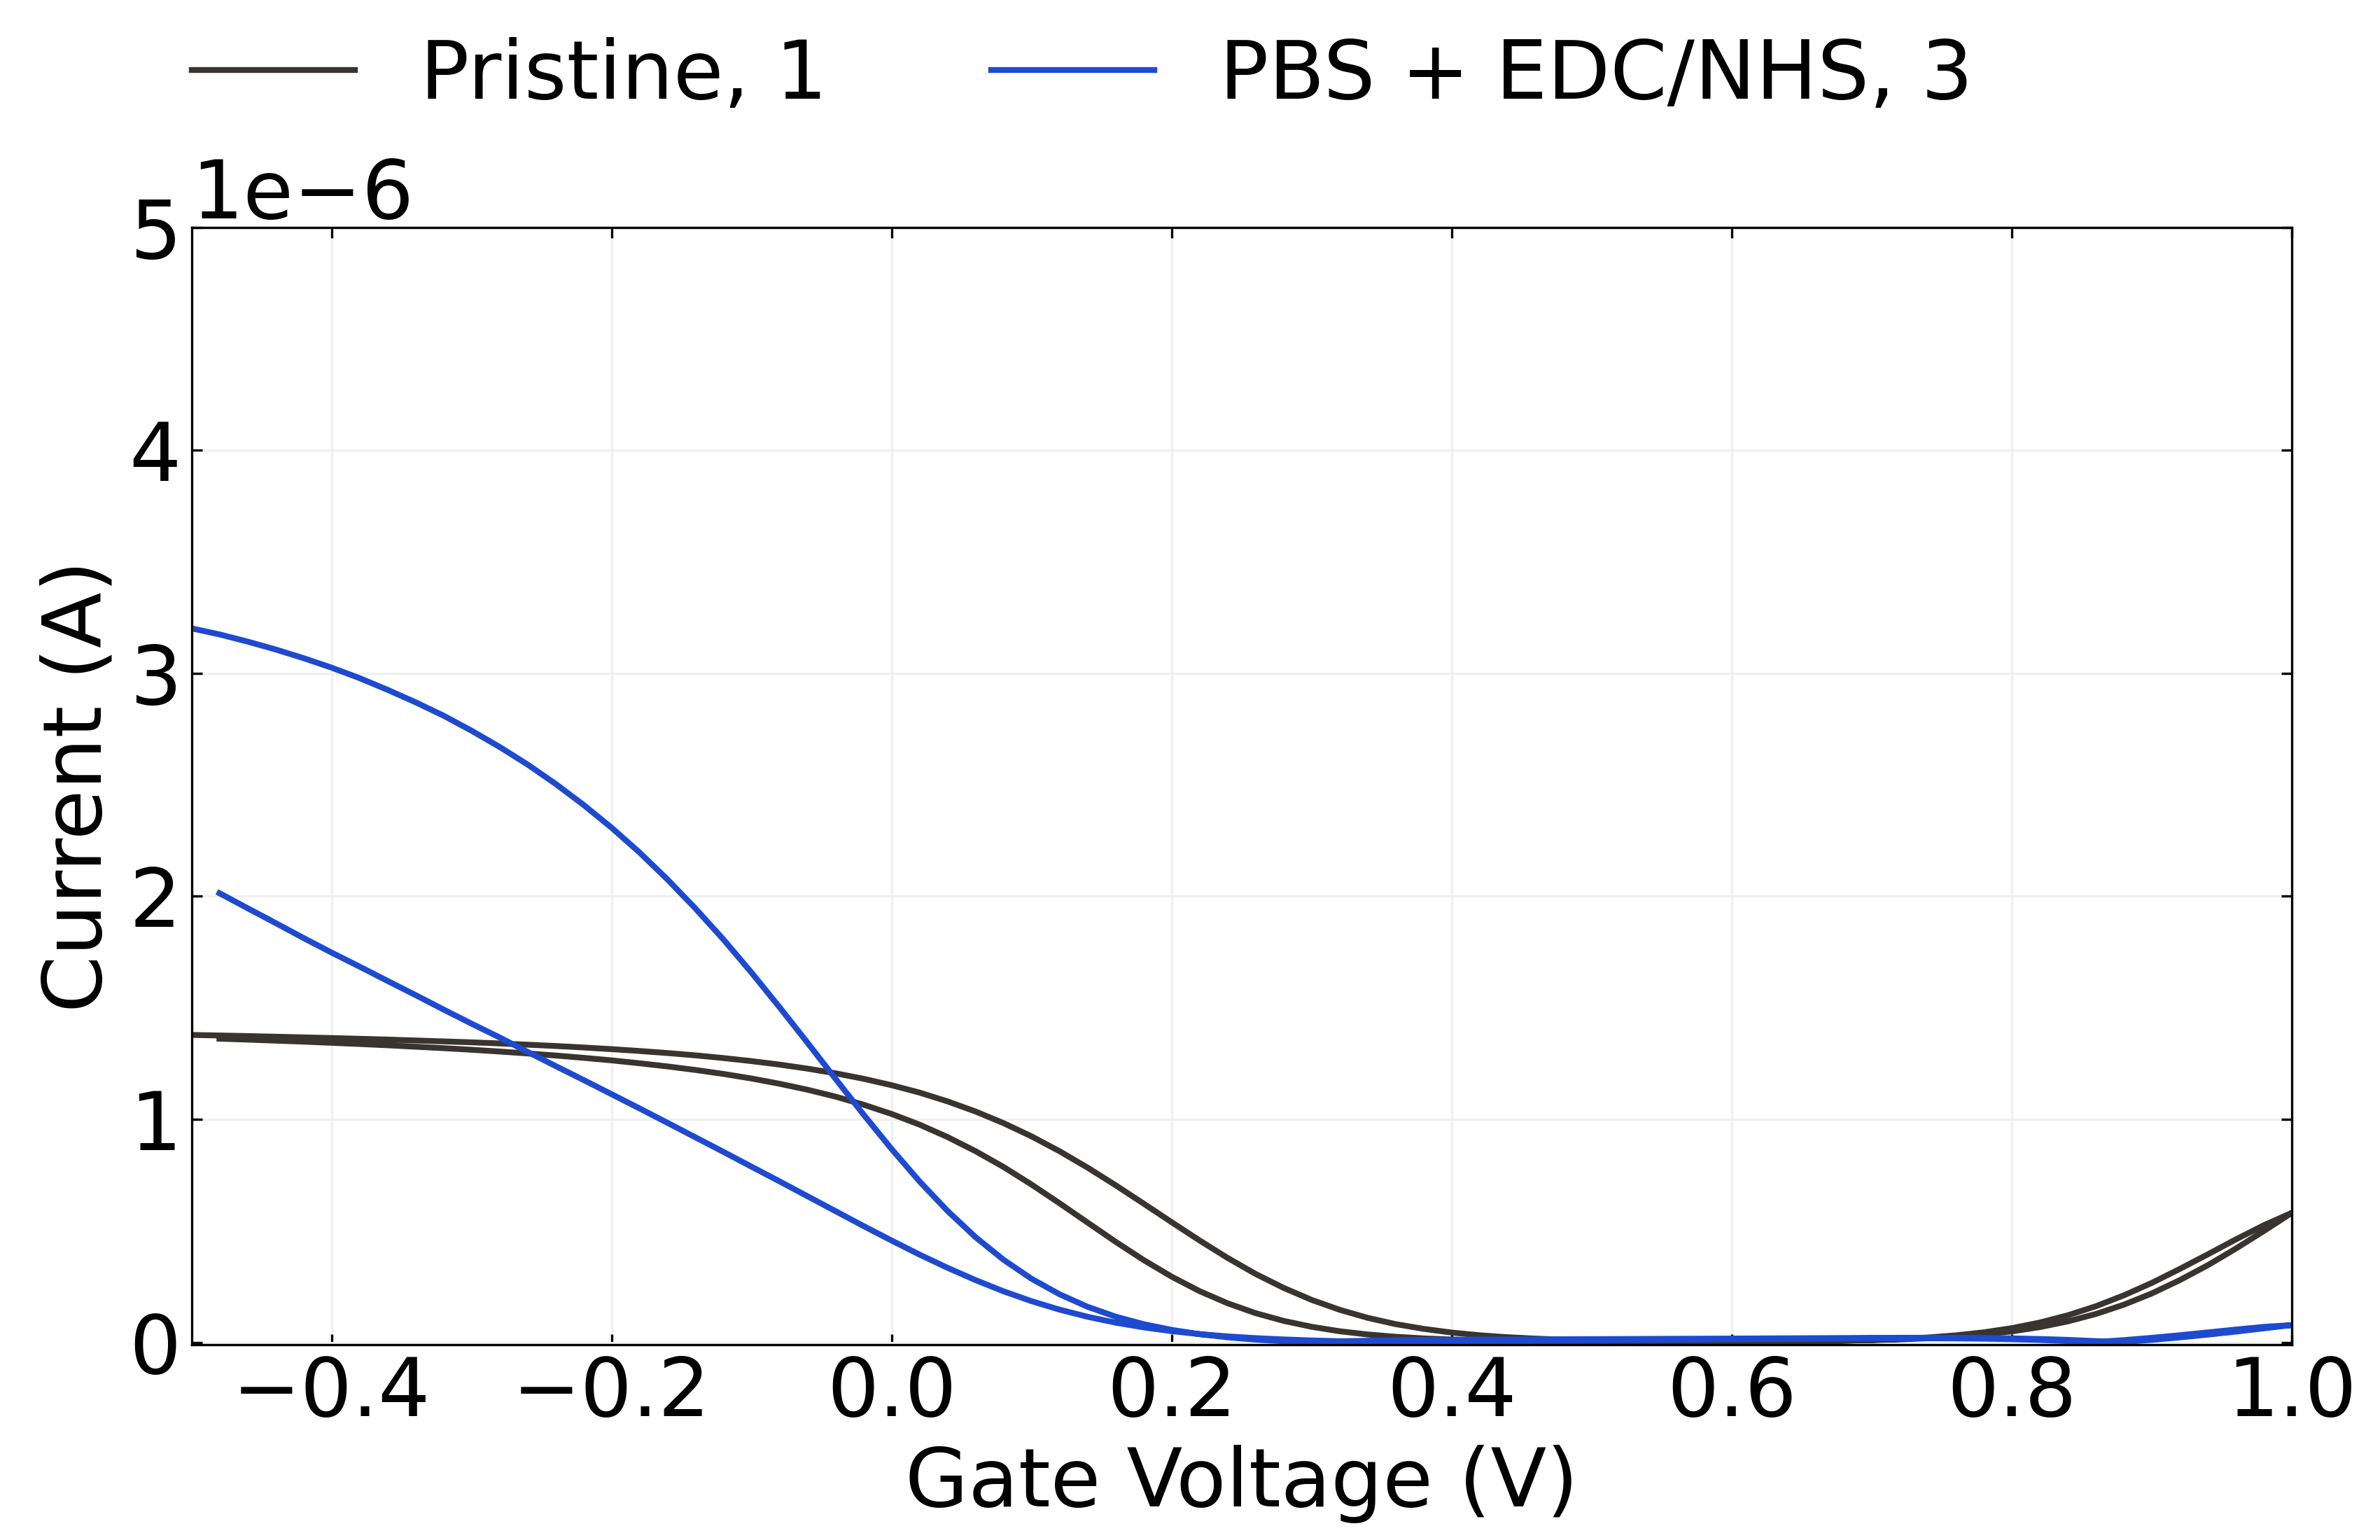
\includegraphics{figures/ch7/NTQ24C10_ch3_comparison_2.png}

}

}

\subcaption{\label{fig-edc-nhs-threshold-shift}}
\end{minipage}%
\newline
\begin{minipage}[t]{0.50\linewidth}

{\centering 

\raisebox{-\height}{

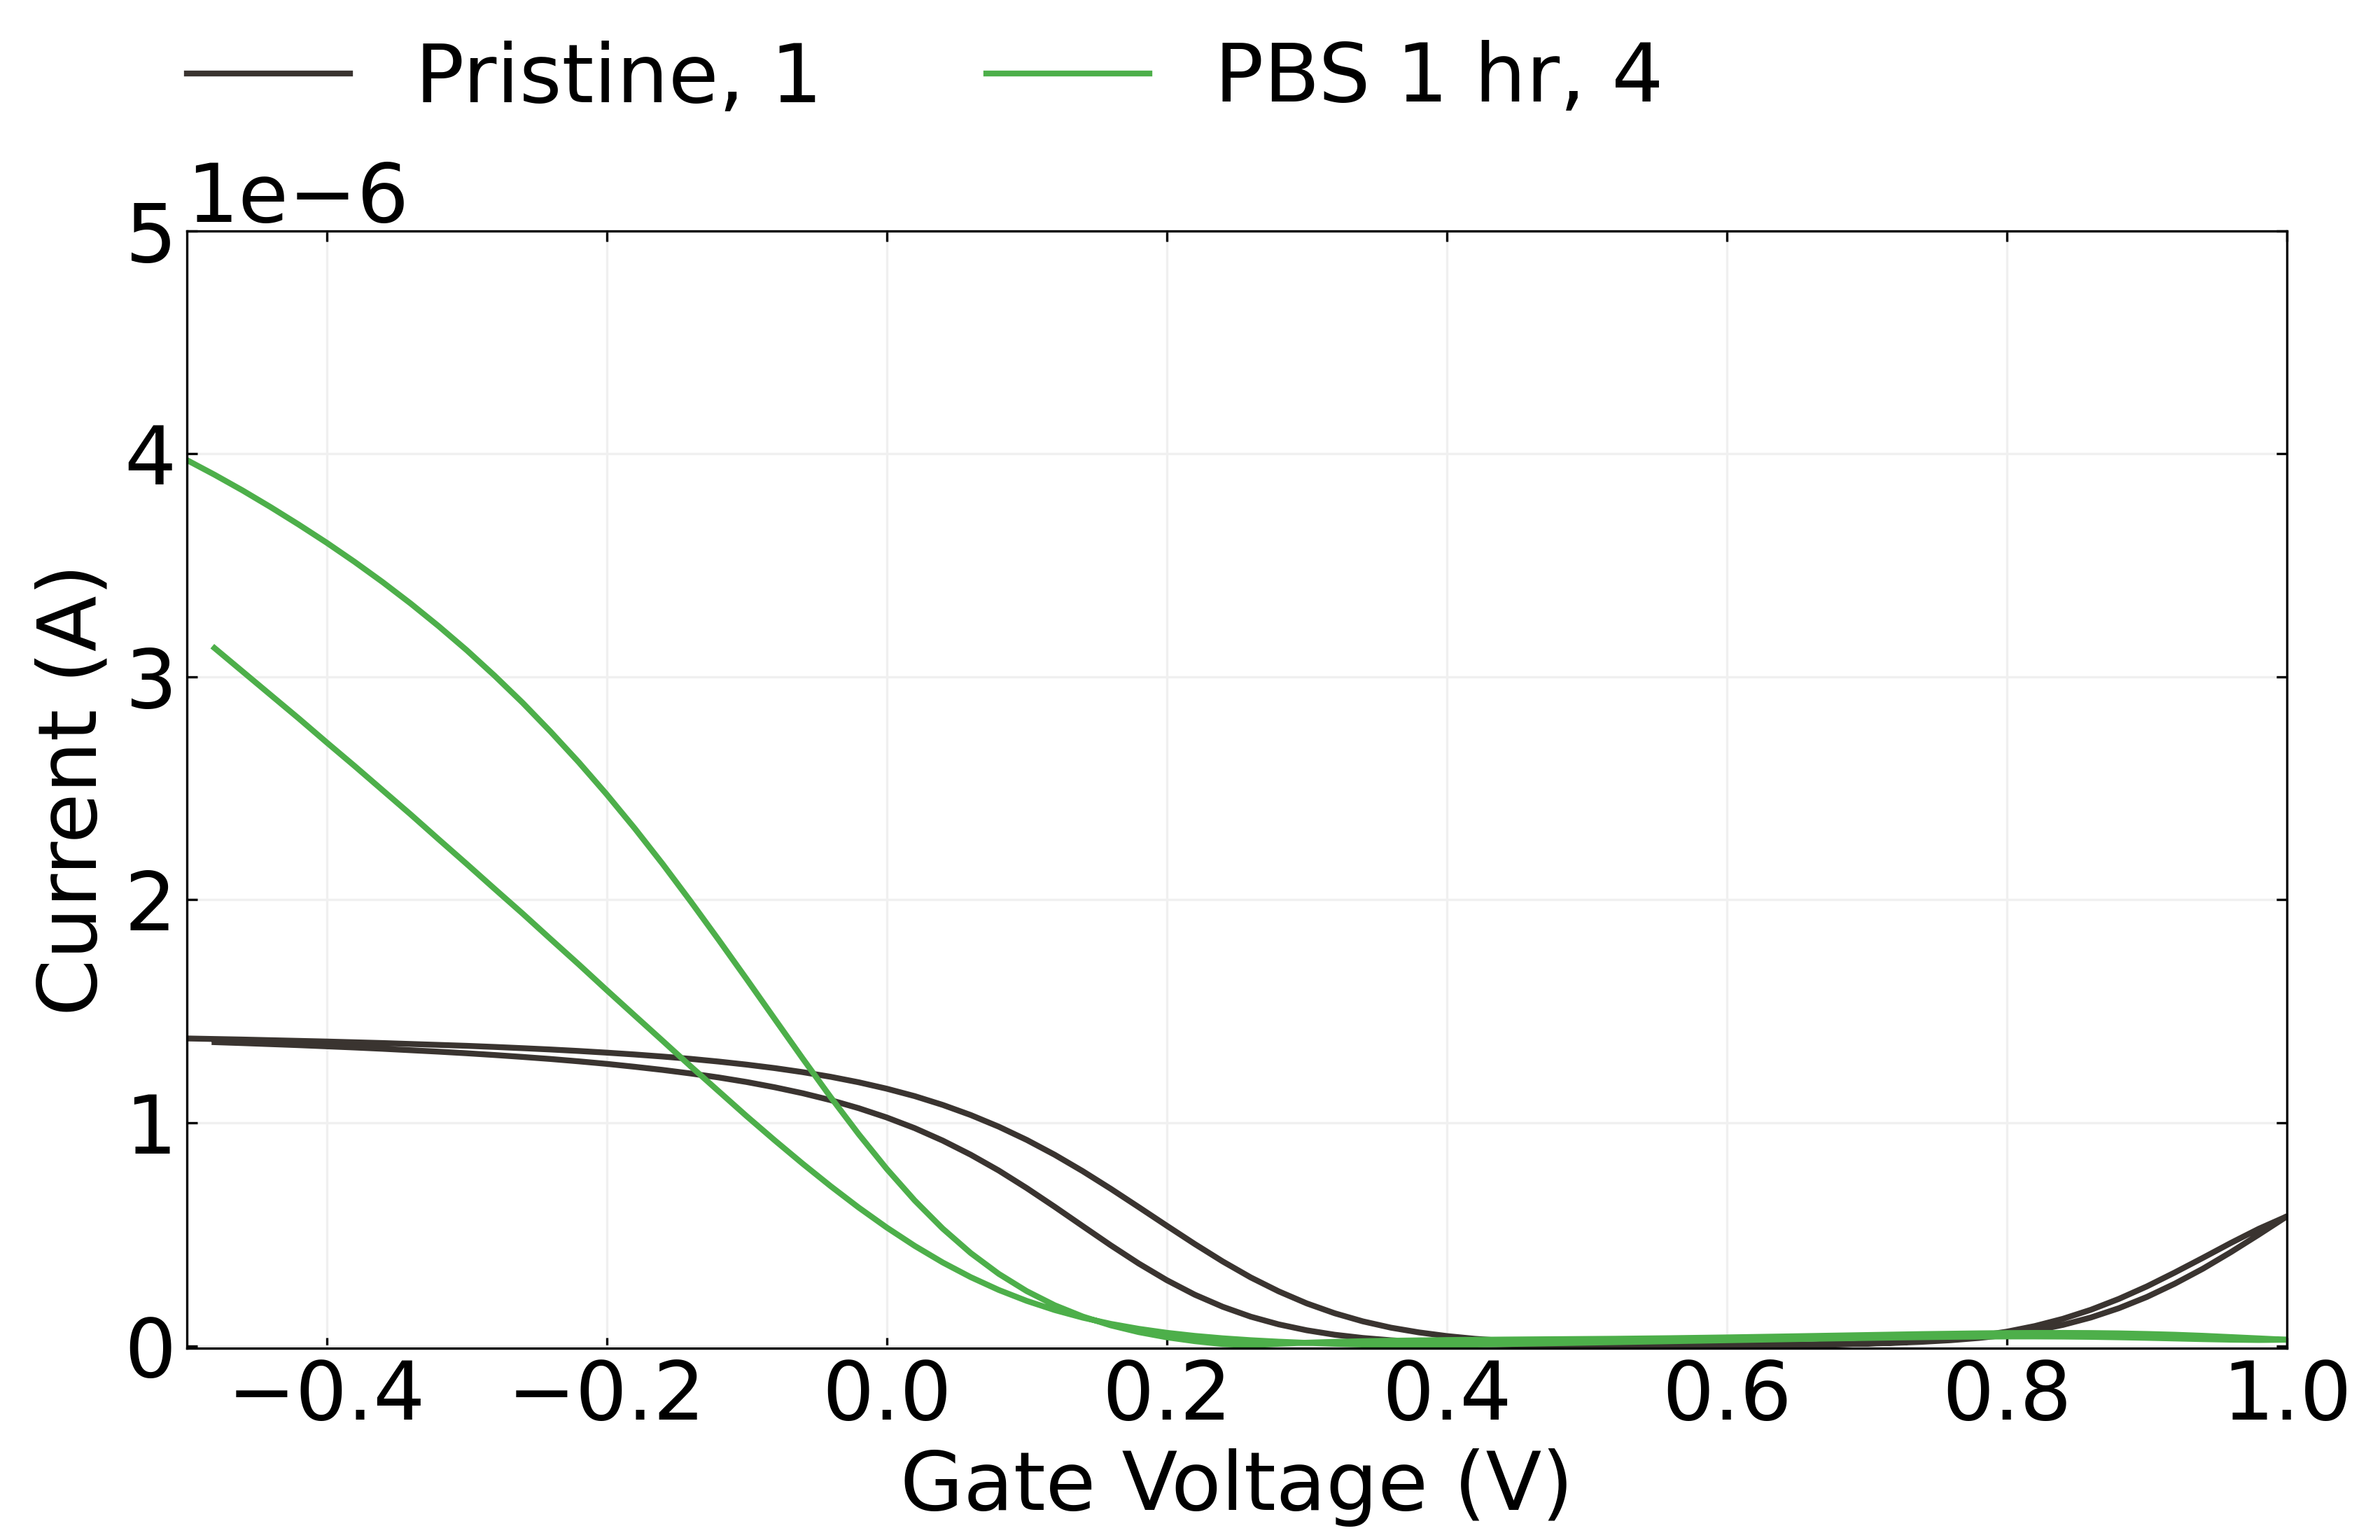
\includegraphics{figures/ch7/NTQ24C10_ch3_comparison_3.png}

}

}

\subcaption{\label{fig-rinse-threshold-shift}}
\end{minipage}%
%
\begin{minipage}[t]{0.50\linewidth}

{\centering 

\raisebox{-\height}{

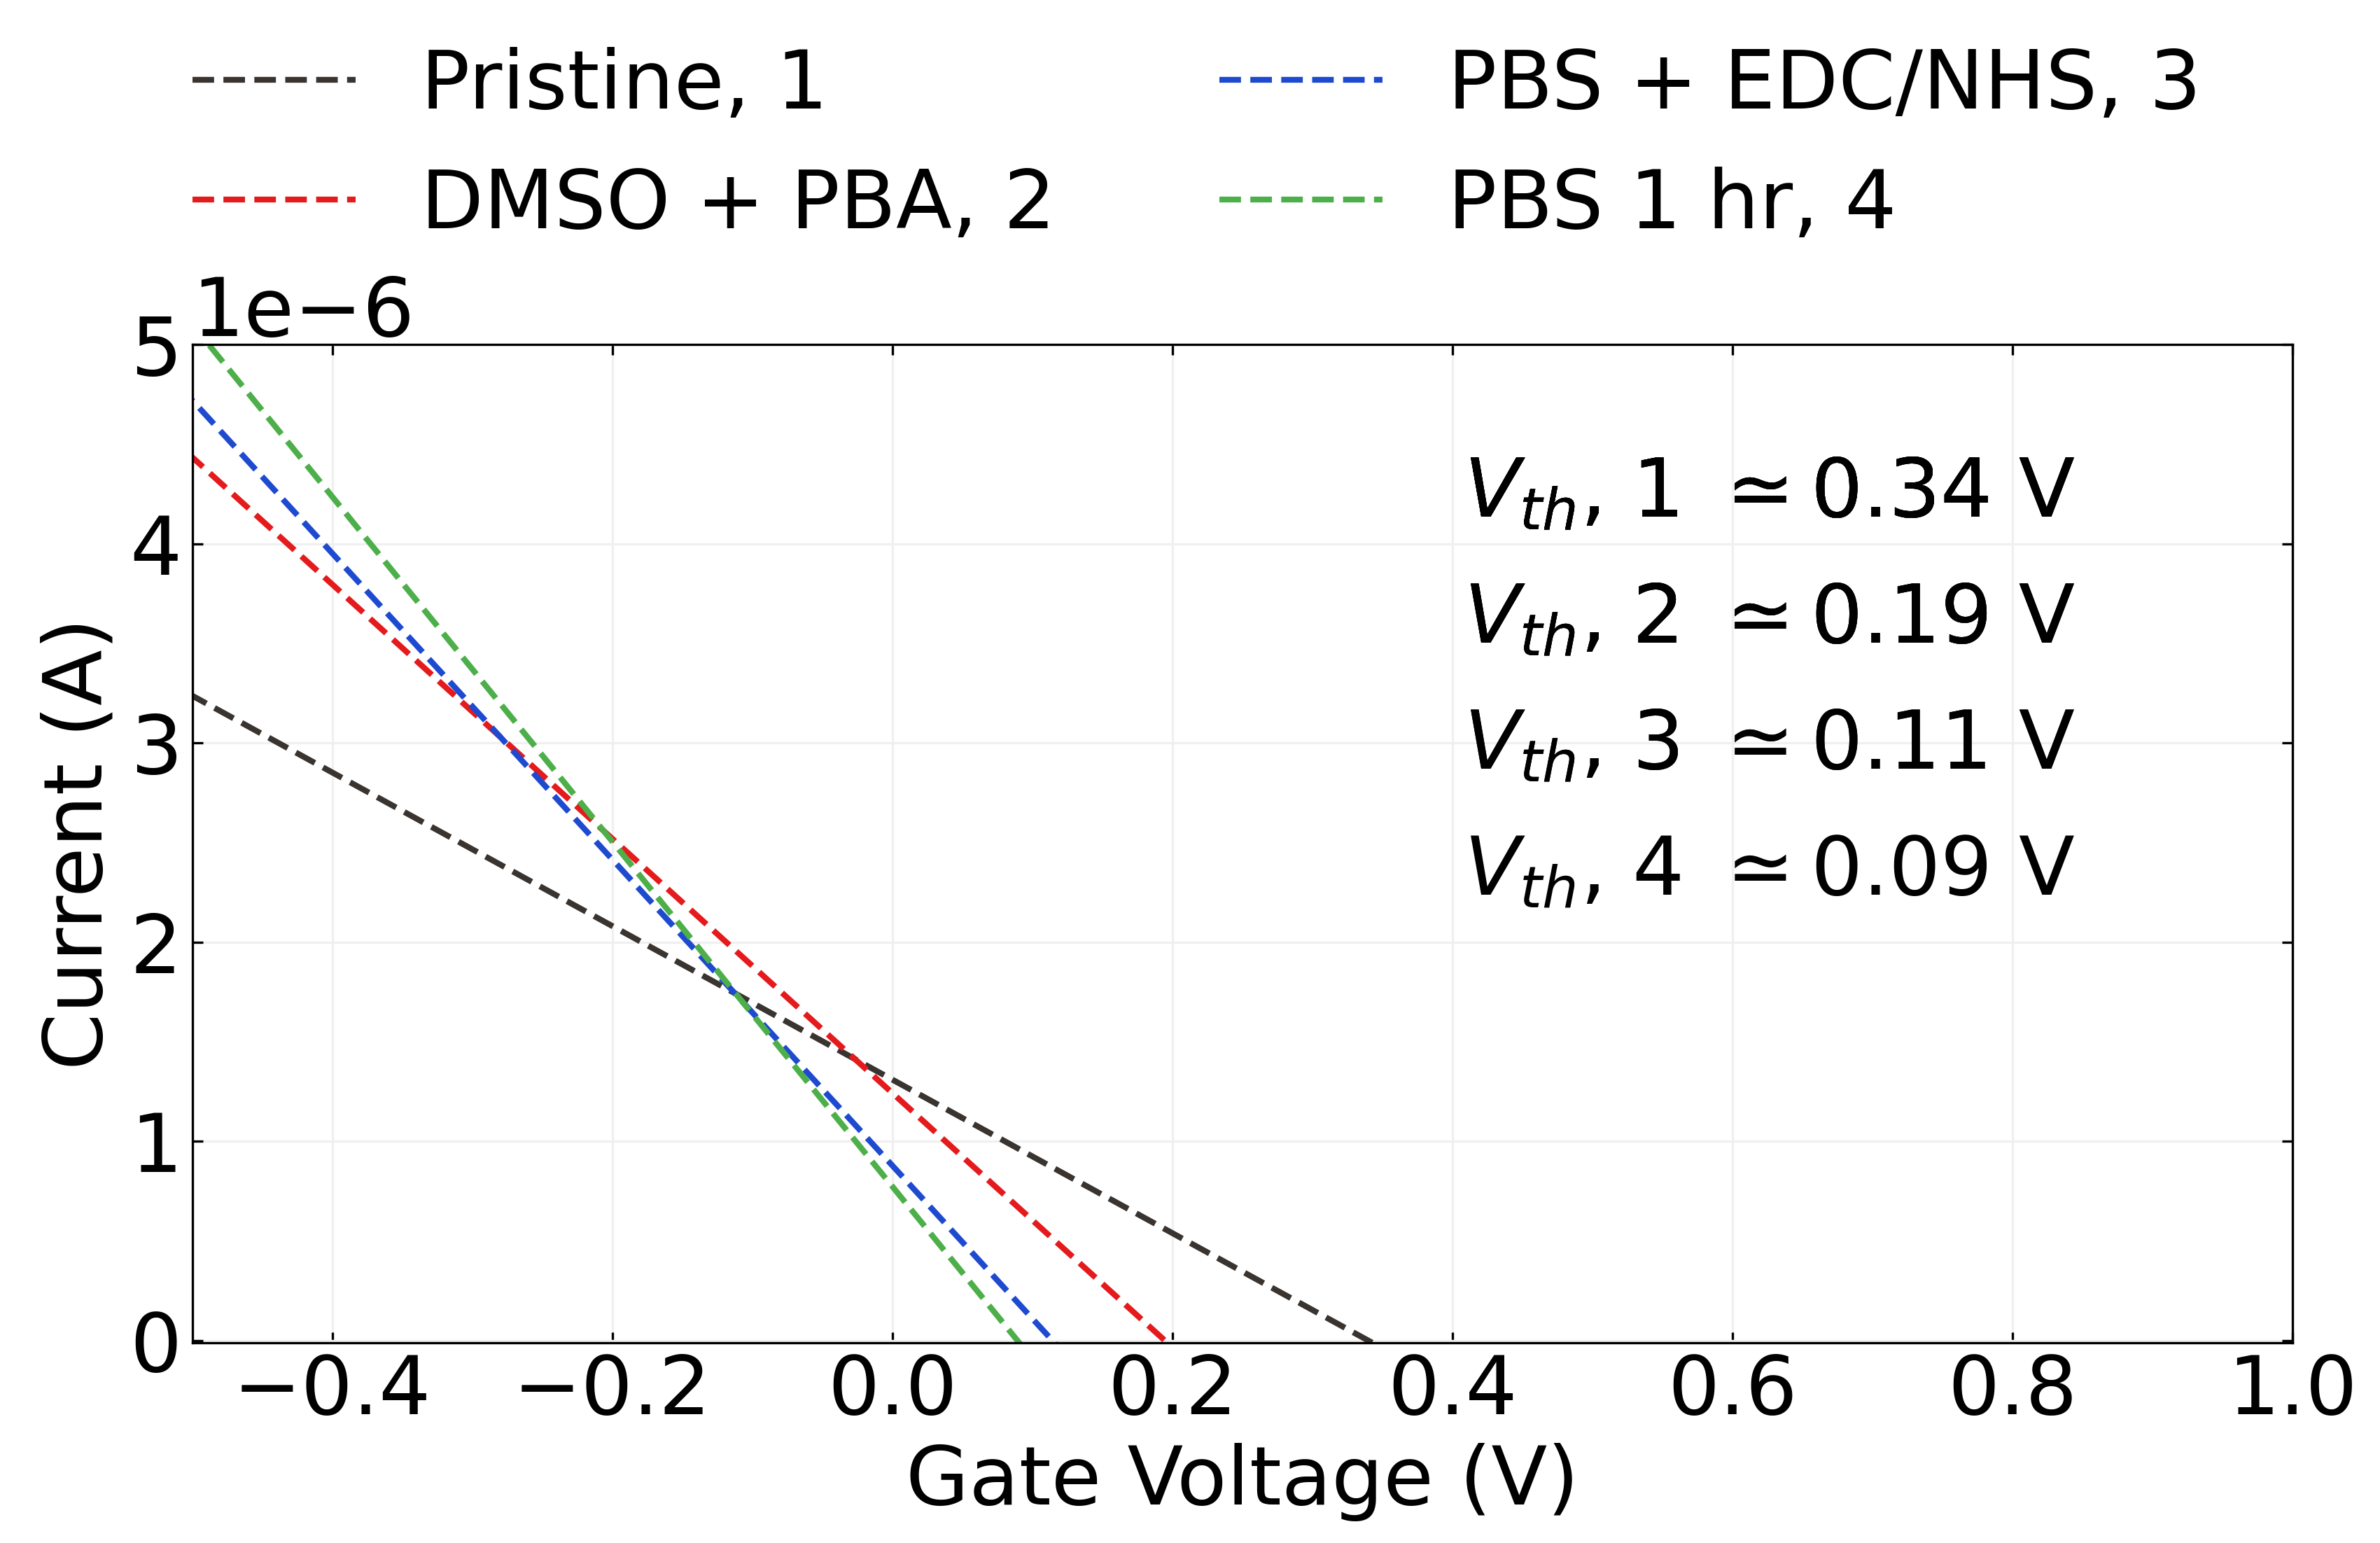
\includegraphics{figures/ch7/NTQ24C10_ch3_comparison_4.png}

}

}

\subcaption{\label{fig-pba-threshold-shift-comparison}}
\end{minipage}%

\caption{\label{fig-pba-functionalisation-threshold-shift}Electrical
transfer characteristics of a carbon nanotube transistor before
functionalisation alongside the transfer characteristics (a) after being
submerged in DMSO containing 5 mM PBA for 1 hour in red, (b) after being
submerged in 1XPBS containing 20 mM EDC and 40 mM NHS for 30 min in
blue, and (c) after being submerged in fresh 1XPBS for 1 hour in green.
The linear fits to the subthreshold slope of each characteristic curve
are shown in (d) as dashed lines, alongside the threshold voltages
calculated by finding the intercept of each fit.}

\end{figure}

There is a \(\sim 3 \times\) increase in the intensity ratio
I\(_D\)/I\(_G\) for both the films modified with PBASE and PBA compared
to the film which was only exposed to DMSO. Previous works have found
that a change in the intensity ratio indicates successful
\(\pi\)-stacking on the carbon nanotube surface, as it indicates surface
modification of the carbon nanotubes has occurred {[}@Wei2010;
@Lan2013{]}. Wei \emph{et al.} {[}@Wei2010{]} found functionalisation
with PBASE altered the ratio by a factor of \(\sim 1.5 \times\), while
Lan \emph{et al.} {[}@Lan2013{]} found that functionalisation with PBA
altered the ratio by a factor of \(\sim 0.8 \times\). The reason for the
large difference between results is not immediately clear, but may
result from the significant differences in the pristine composition and
morphology of carbon nanotube networks used in each publication, and
differences in the functionalisation method used. Across all scan
locations in \textbf{?@fig-raman-comparison}, the value found for
I\(_D\)/I\(_G\) is consistently \(\sim 0.095\) for both PBA and PBASE.
Furthermore, subsequent Raman measurements of the PBA-modified film
after further functionalisation with EDC/NHS do not show a significant
change in I\(_D\)/I\(_G\). These results indicate that presence of the
NHS ester has little effect on the Raman shift. It should be clarified
that Raman spectroscopy cannot be used to distinguish between the
presence of PBA and PBASE on the device surface. However, it is clear
that functionalisation of the carbon nanotube network with both the PBA
and PBASE has led to measurable \(pi\)-stacking between the network and
the pyrene group attached to each compound.

\hypertarget{electrical-characterisation-1}{%
\subsubsection{Electrical
Characterisation}\label{electrical-characterisation-1}}

Figure~\ref{fig-pba-functionalisation-threshold-shift} shows the
transfer characteristics of a carbon nanotube transistor channel at
various stages of a PBA/EDC functionalisation, where a excess of
N-hydroxysuccinimide (NHS) was added alongside EDC. A solvent-deposited
carbon nanotube film was used for the device. The PBA was dissolved in
DMSO, and the device channels were exposed to this solution for 1 hour.
The electrical change resulting from PBA exposure is shown in
Figure~\ref{fig-pba-threshold-shift}. The threshold shift with the
addition of 5 mM PBA in DMSO for 1 hour is equivalent to the shift seen
when only DMSO is added, \(\Delta\)V = -0.15 V. The lack of a
significant threshold shift directly attributable to the PBA is a result
of pyrene having a neutral charge state; any contributions from the
charged carboxyl group are screened from the carbon nanotube sidewalls
by surrounding water molecules {[}@Lerner2012{]}. However, as in the
case of the addition of PBASE, there also appears to be an increase in
hole mobility, which may be due to the pyrene groups increasing
connectivity within the carbon nanotube network {[}@Murugathas2019b{]}.

Subsequently, the device was rinsed with 1XPBS and exposed to 20 mM EDC
and 40 mM NHS in 1XPBS electrolyte for 30 minutes.
Figure~\ref{fig-edc-nhs-threshold-shift} shows the change resulting from
subsequent EDC/NHS exposure. When EDC/NHS is added, a threshold shift of
\(\Delta\)V \(\sim\) -0.08 V was observed on multiple channels. The
exposure to EDC/NHS negatively shifts the transfer characteristic curve,
most likely due to the PBA present reacting to form positively-charged
\emph{O}-acylisourea esters and negatively gating the attached carbon
nanotube network {[}@Heller2008; @Hermanson2013-4{]}.
Figure~\ref{fig-rinse-threshold-shift} shows that this shift is not
significantly affected by further exposure of the channel to PBS. This
indicates that hydrolysis over the course of one hour is insufficient to
hydrolyse a significant proportion of the \emph{O}-acylisourea back to
PBA, as PBA is charge neutral. We therefore expect that the a
significant amount of \emph{O}-acylisourea remains active within this
time period and available for reaction with biomolecule amine groups.

\hypertarget{attachment-of-peglyated-pyrene-based-linkers}{%
\subsection{Attachment of PEGlyated Pyrene-Based
Linkers}\label{attachment-of-peglyated-pyrene-based-linkers}}

\hypertarget{sec-NTA-biotin-PEG}{%
\subsubsection{Pyrene-NTA, Pyrene-Biotin and
PEGylation}\label{sec-NTA-biotin-PEG}}

Through chemical coupling/conjugation, it is possible to replace the NHS
ester group on PBASE with other groups that can undergo binding
reactions with proteins. Unlike PBASE, these groups do not suffer the
drawback of being readily hydrolysed. For example, PBASE can be modified
with N\(\alpha\),N\(\alpha\)-Bis(carboxymethyl)-L-lysine hydrate (also
known as N-(5-Amino-1-carboxypentyl)iminodiacetic acid, AB-NTA) to
produce pyrene-nitrilotriacetic acid (pyrene-NTA). The attached NTA
group is able to chelate with metal ions such as Cu\(^{2+}\) or
Ni\(^{2+}\), which then can then coordinate with polyhistidine-tags
attached to a protein {[}@Holzinger2011; @Amano2016; @Chang2017{]}. Use
of Cu\(^{2+}\) ions over Ni\(^{2+}\) gives stronger histidine bonding
and less non-specific adsorption {[}@Chang2017{]}. Functionalisation
using the NTA-Ni\(^{2+}\) chemistry was successfully used to attach
mammalian odorant receptors to a single carbon nanotube for detection of
eugenol vapour in real-time {[}@Goldsmith2011{]}. Pyrene-biotin (pyrene
butanol biotin ester) can also be produced for attaching avidin or
strepavidin {[}@Holzinger2011{]}. As avidin and strepavidin are
tetrameric, they can be attached to both pyrene-biotin and biotinylated
avi-tagged proteins simultaneously via strong non-covalent bonding,
therefore linking the transducer and receptor {[}@Star2003a;
@Dundas2013; @Hermanson2013-11; @Fairhead2015{]}. As the presence of
his-tags and avi-tags on proteins can be readily controlled, these
methods offer improved specificity and directionality over the
traditional amide bonding seen earlier.

It is also possible to attach polyethylene glycol (PEG) chains to a
pyrene group and modify them with reactive groups such as NTA and biotin
to attach proteins in the manner outlined in the previous paragraph
{[}@Hermanson2013-18; @Meran2018{]}. Once modified with PEG, the water
solubility of pyrene linkers increases, making it possible to perform a
full functionalisation procedure exclusively in aqueous solution
{[}@Hermanson2013-18{]}. By setting the length of the PEG chain, the
size of the linker molecule can be controlled - selection of a short
chain is important for ensuring attached receptors remain within the
Debye length of the transducer {[}@Shkodra2021{]}. Functionalisation of
a graphene transducer with pyrene-PEG-biotin has previously been used to
bind streptavidin to a graphene field-effect transistor device
{[}@Miki2019{]}. The PEGlyated linkers used in the following sections
were purchased pre-prepared. Pyrene-PEG-NTA (2 kDa) was purchased from
Nanocs, while pyrene-PEG-FITC (2 kDa, 10 kDa), pyrene-PEG-rhodamine (3.4
kDa), mPEG-Pyrene (10 kDa) and pyrene-PEG-biotin (10 kDa) were purchased
from Creative PEGworks.

\hypertarget{sec-impediments}{%
\subsection{Identifying Functionalisation Issues using Fluorescence
Microscopy}\label{sec-impediments}}

\hypertarget{sec-fluorescence-remarks}{%
\subsubsection{General Overview}\label{sec-fluorescence-remarks}}

Various dyes and fluorescent tags were used to investigate approaches
for identifying successful attachment of biomolecules to a carbon
nanotube or graphene surface with fluorescence microscopy. The dyes
included fluorescein isothiocyanate (FITC), Rhodamine B and Cyanine 3
(Cy3). Green fluorescent protein was also used for this testing process.
It is important to note that these dyes and the GFP chromophore all
contain benzene rings which are able to \(\pi\)-stack with carbon rings
to some degree {[}@Nakayama-Ratchford2007; @Tang2012;@Khrenova2019;
@Qiu2019{]}. However, there is also significant variation in the
effectiveness of this \(\pi\)-stacking, as shown by
Figure~\ref{fig-FITC-rhodamine-B}. Here, a clear, specific interaction
is seen between Rhodamine B and graphene, but little interaction between
FITC and graphene is observed, even when a longer exposure time is used.
Whether the addition of pyrene linker groups these dyes, or dye-modified
biomolecules, was therefore investigated in further detail. This process
then led to the identification of multiple issues that could impede a
successful device functionalisation.

\begin{figure}

\begin{minipage}[t]{0.47\linewidth}

{\centering 

\raisebox{-\height}{

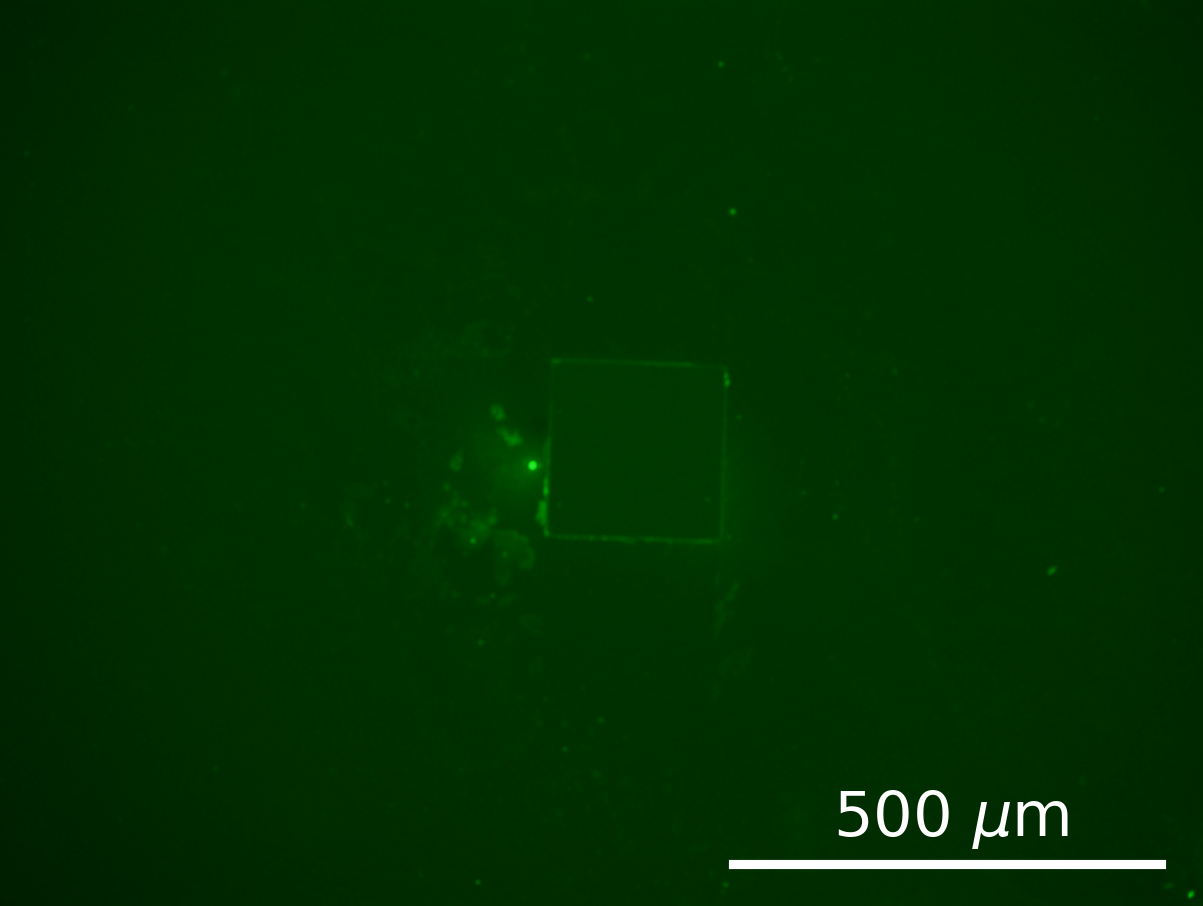
\includegraphics{figures/ch7/NGW8D1_FITC_6.5sexposure_10X_221121.png}

}

}

\subcaption{\label{fig-FITC}}
\end{minipage}%
%
\begin{minipage}[t]{0.05\linewidth}

{\centering 

~

}

\end{minipage}%
%
\begin{minipage}[t]{0.47\linewidth}

{\centering 

\raisebox{-\height}{

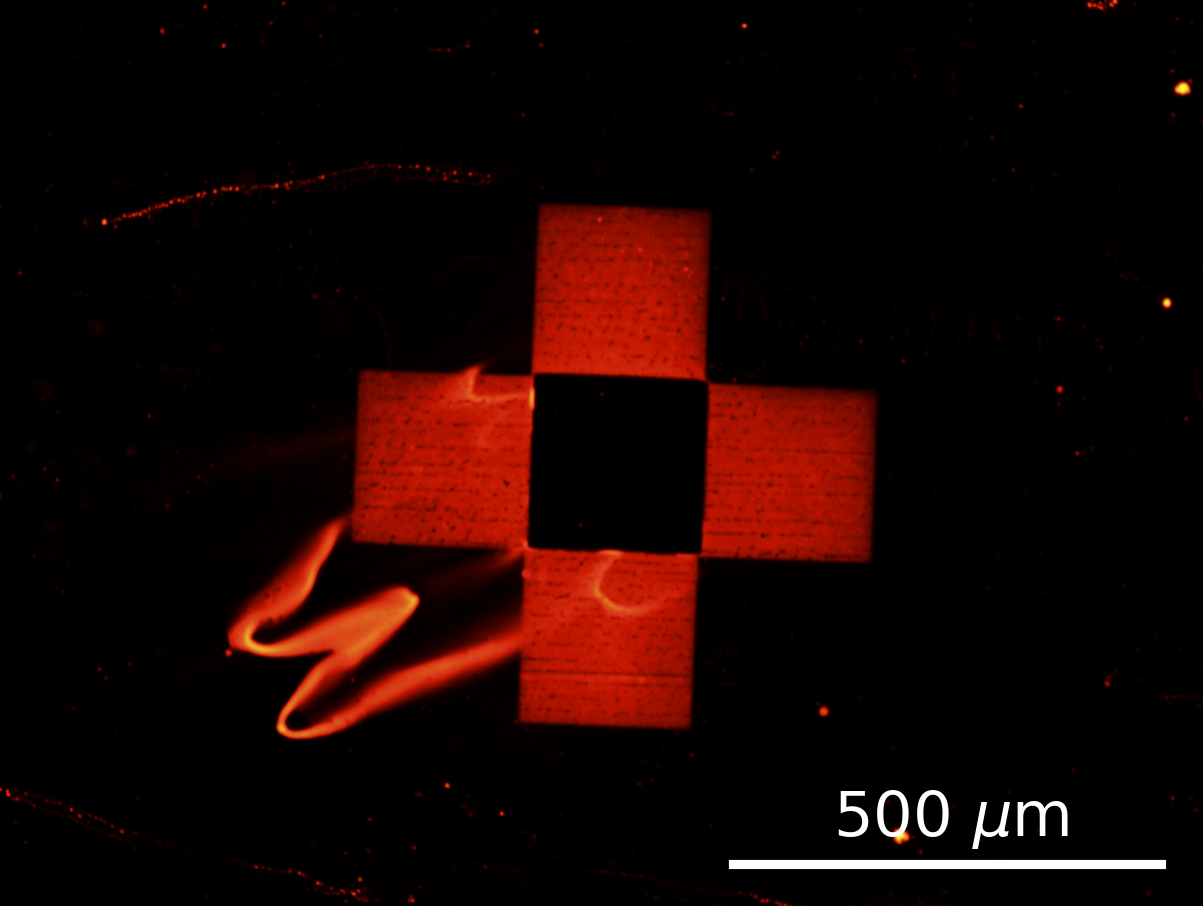
\includegraphics{figures/ch7/NGW8D4_rhodamineB_cornergraphene_221110.png}

}

}

\subcaption{\label{fig-rhodamine}}
\end{minipage}%

\caption{\label{fig-FITC-rhodamine-B}Four 200 \(\mu\)m \(\times\) 200
\(\mu\)m graphene squares modified with the dyes (a) fluorescein
isothiocyanate (FITC) and (b) Rhodamine B. No pyrene/PEG/pyrene-PEG was
attached to these dyes. In (a), an FITC filter and 6.5 s exposure time
was used, and in (b) a Texas Red filter and 1.4 s exposure time was
used.}

\end{figure}

Both SU8 and AZ\(^\circledR\) 1518 photoresist fluoresced under a
variety of microscope filters, resulting from light interacting with the
photoactive component present in both resists {[}@Pai2007{]}. This
background fluorescence was found to drown out fluorescence from a
dye-functionalised device channel, and so photoresist encapsulated
devices were not used for fluorescence imaging. (Consider a photograph
of a dim outdoor lamp; if the photograph was taken on a starless night,
the light from the lamp would show up clearly, but with the sun out the
light would be very difficult to see regardless of how the photograph
was taken.) A different type of encapsulation could potentially be used
to verify linker attachment with fluorescence after a device has been
encapsulated. These alternative encapsulation methods for use with
fluorescence microscopy are discussed in \textbf{?@sec-future-work}.

\hypertarget{sec-photoresist-contamination}{%
\subsubsection{Photoresist
Contamination}\label{sec-photoresist-contamination}}

\begin{figure}

\begin{minipage}[t]{0.47\linewidth}

{\centering 

\raisebox{-\height}{

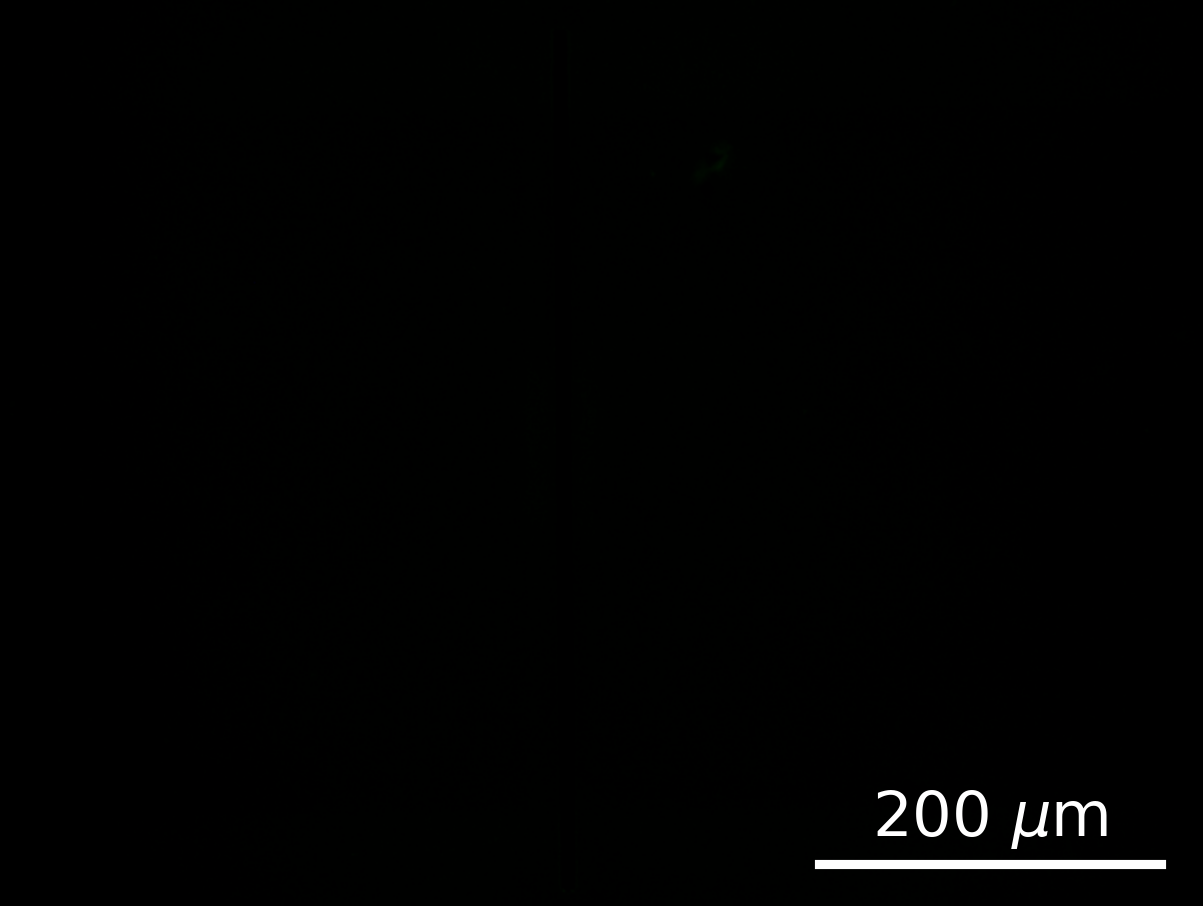
\includegraphics{figures/ch7/modified_SU8only_FITCfilter_channel2_350ms_12.6X_221207.png}

}

}

\subcaption{\label{fig-350ms-SU8}}
\end{minipage}%
%
\begin{minipage}[t]{0.05\linewidth}

{\centering 

~

}

\end{minipage}%
%
\begin{minipage}[t]{0.47\linewidth}

{\centering 

\raisebox{-\height}{

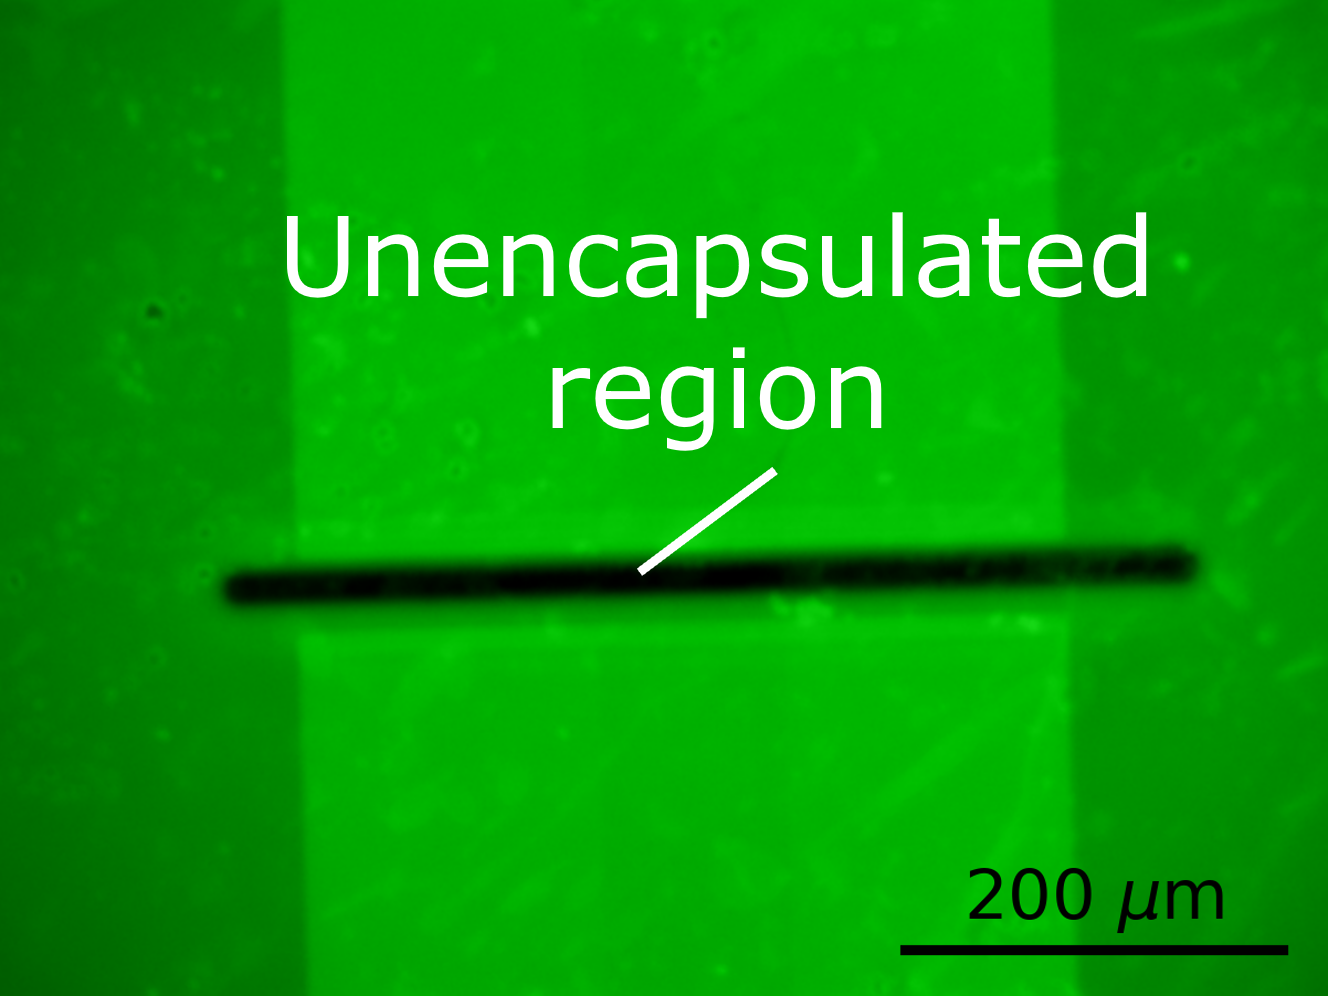
\includegraphics{figures/ch7/modified_CNT20_1mMPPF_channel8_350ms_12.6X_221124.png}

}

}

\subcaption{\label{fig-350ms-SU8-FITC}}
\end{minipage}%
\newline
\begin{minipage}[t]{0.47\linewidth}

{\centering 

\raisebox{-\height}{

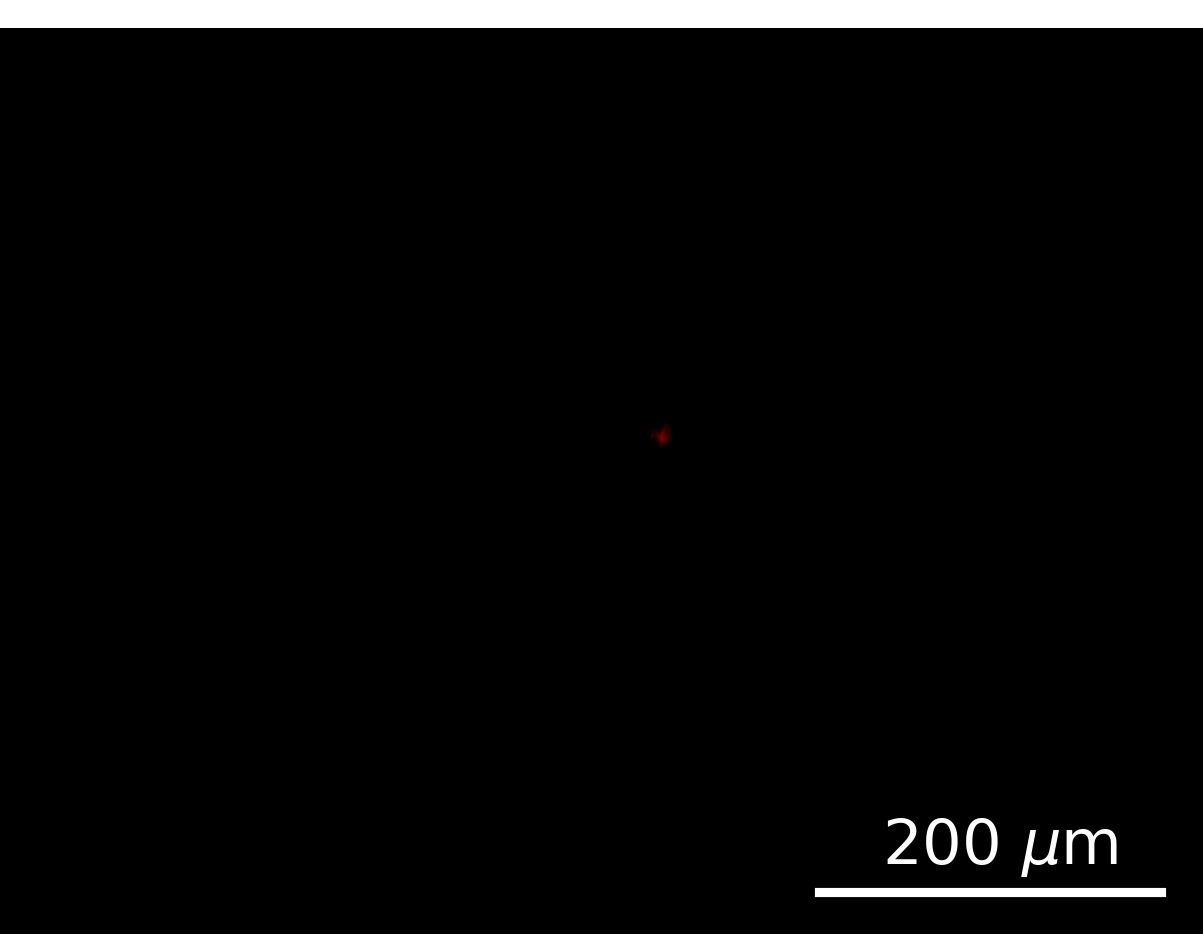
\includegraphics{figures/ch7/modified_Ccontrol_ch2_mCherry_10sexposure_highcontrast_12.6X.png}

}

}

\subcaption{\label{fig-aptamer-photoresist-1}}
\end{minipage}%
%
\begin{minipage}[t]{0.05\linewidth}

{\centering 

~

}

\end{minipage}%
%
\begin{minipage}[t]{0.47\linewidth}

{\centering 

\raisebox{-\height}{

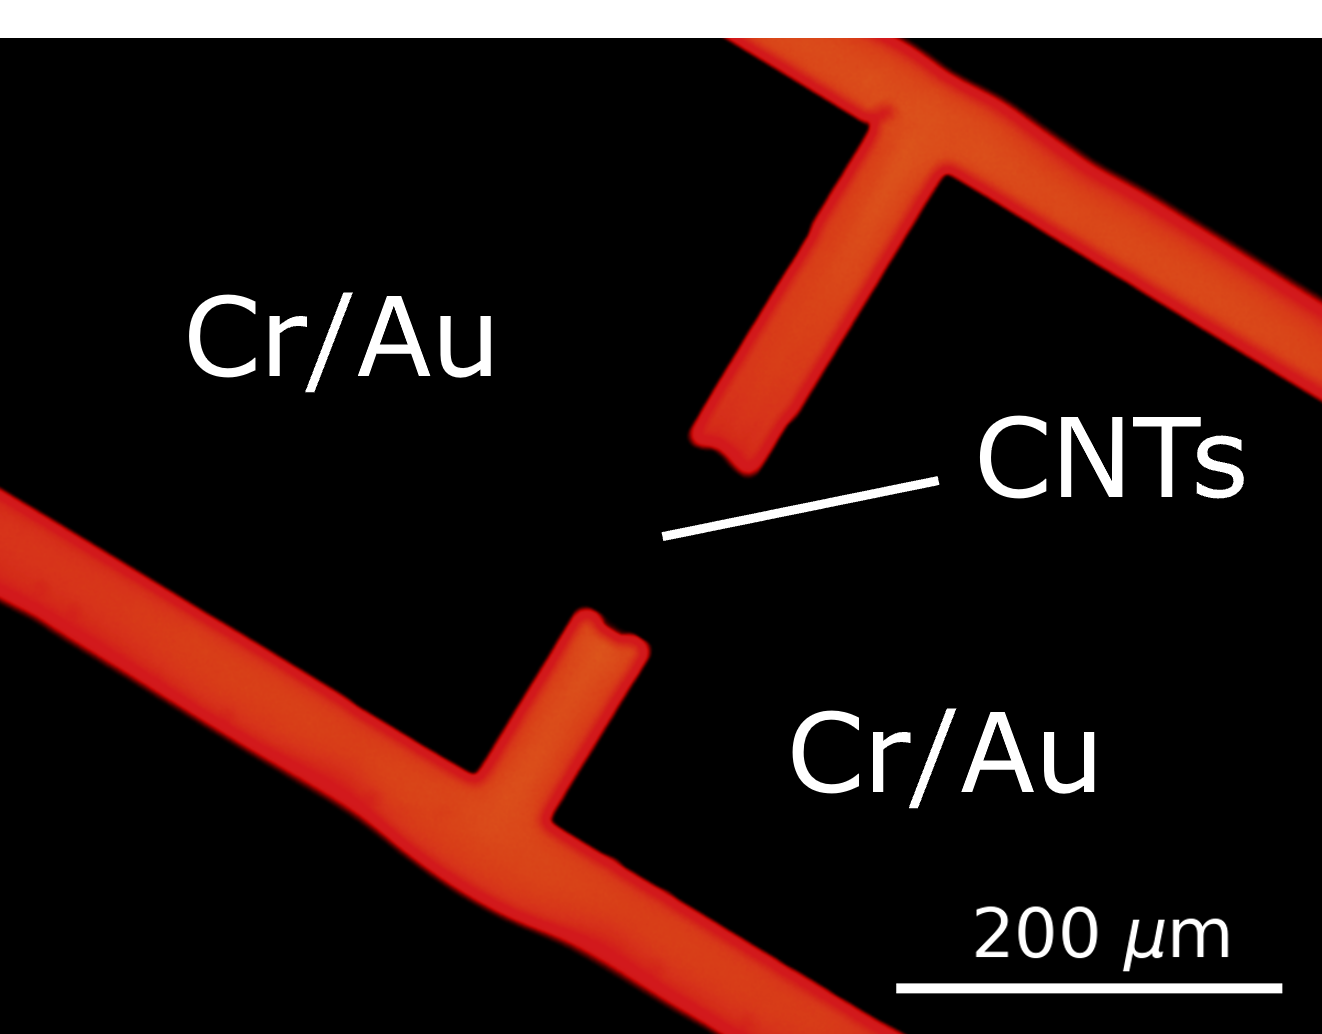
\includegraphics{figures/ch7/modified_C1_ch5_mCherry_10sexposure_highcontrast_12.6X.png}

}

}

\subcaption{\label{fig-aptamer-photoresist-2}}
\end{minipage}%
\newline
\begin{minipage}[t]{0.47\linewidth}

{\centering 

\raisebox{-\height}{

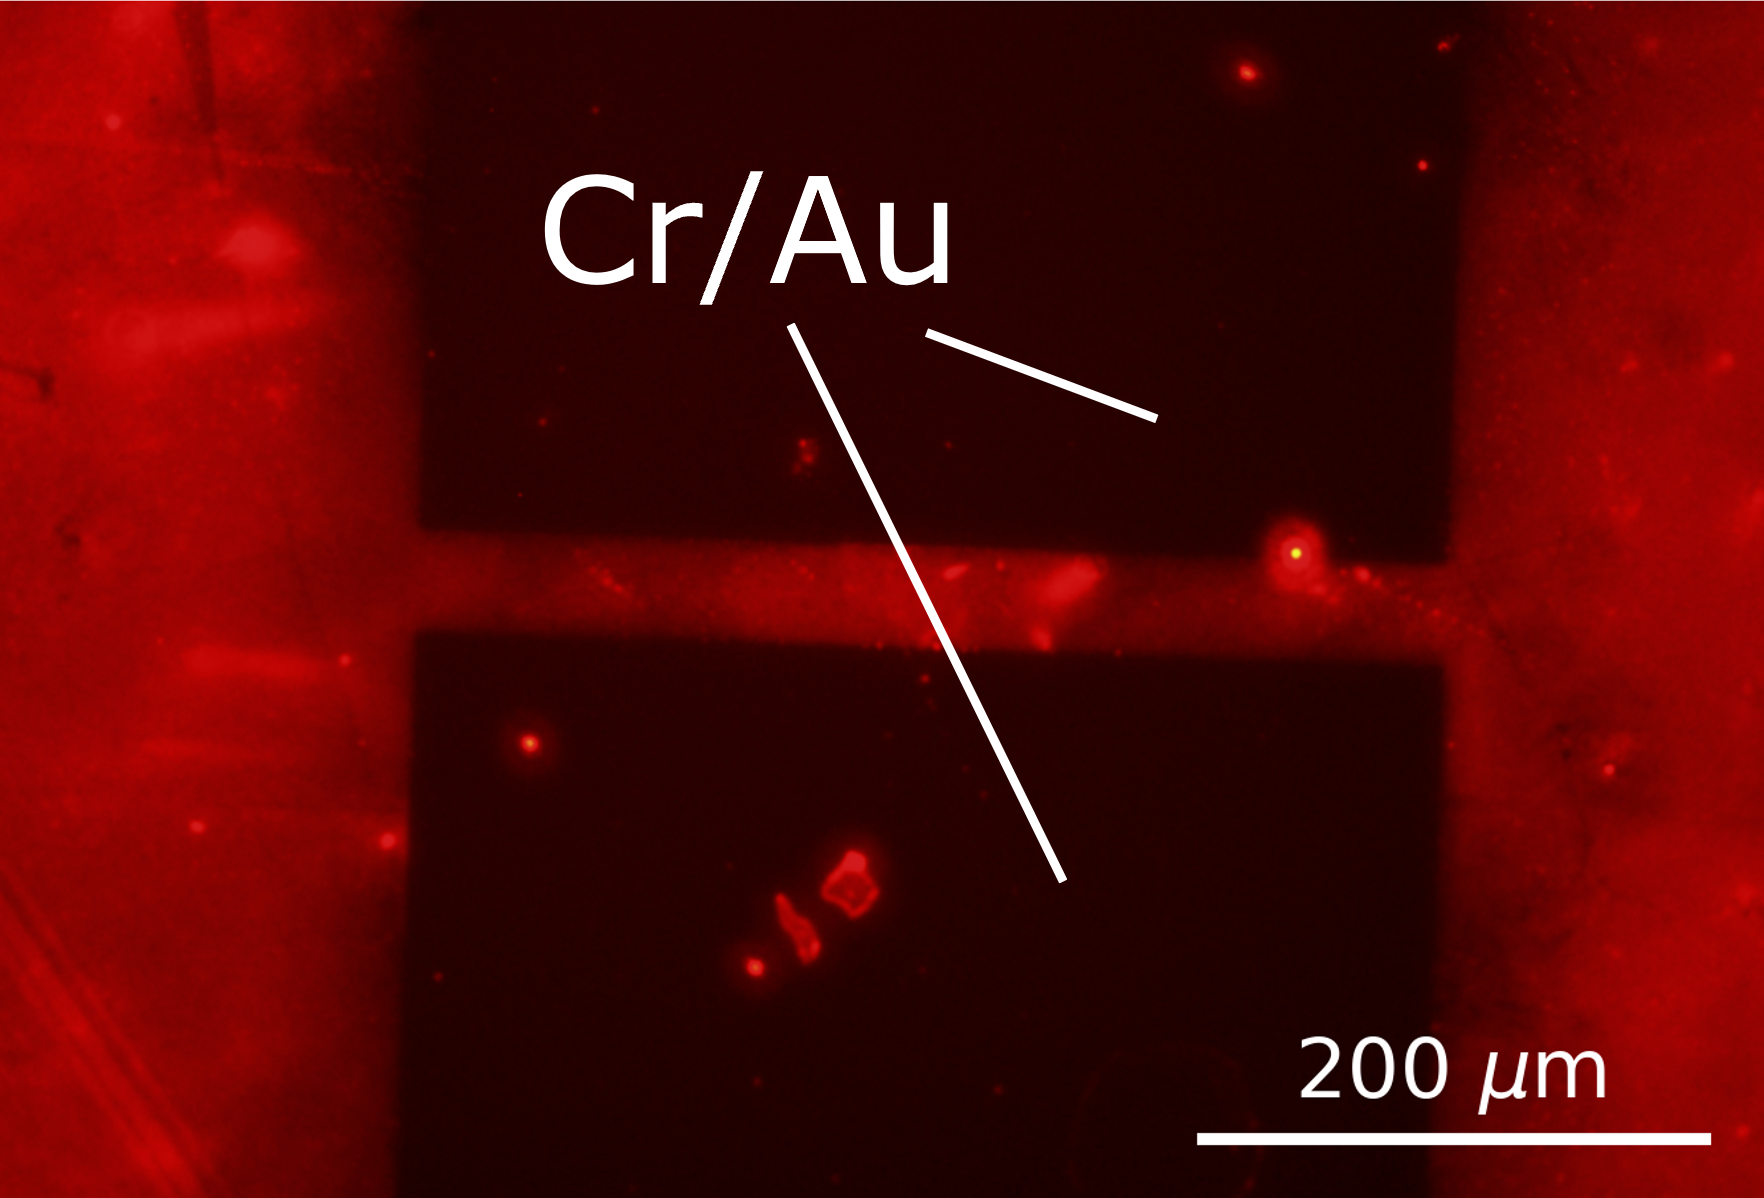
\includegraphics{figures/ch7/modified_softbake1minacetonerinse_aptamer_ch3_mCherry_30sexposure_highcontrast_ISO200_12.6X.png}

}

}

\subcaption{\label{fig-aptamer-photoresist-3}}
\end{minipage}%
%
\begin{minipage}[t]{0.05\linewidth}

{\centering 

~

}

\end{minipage}%
%
\begin{minipage}[t]{0.47\linewidth}

{\centering 

\raisebox{-\height}{

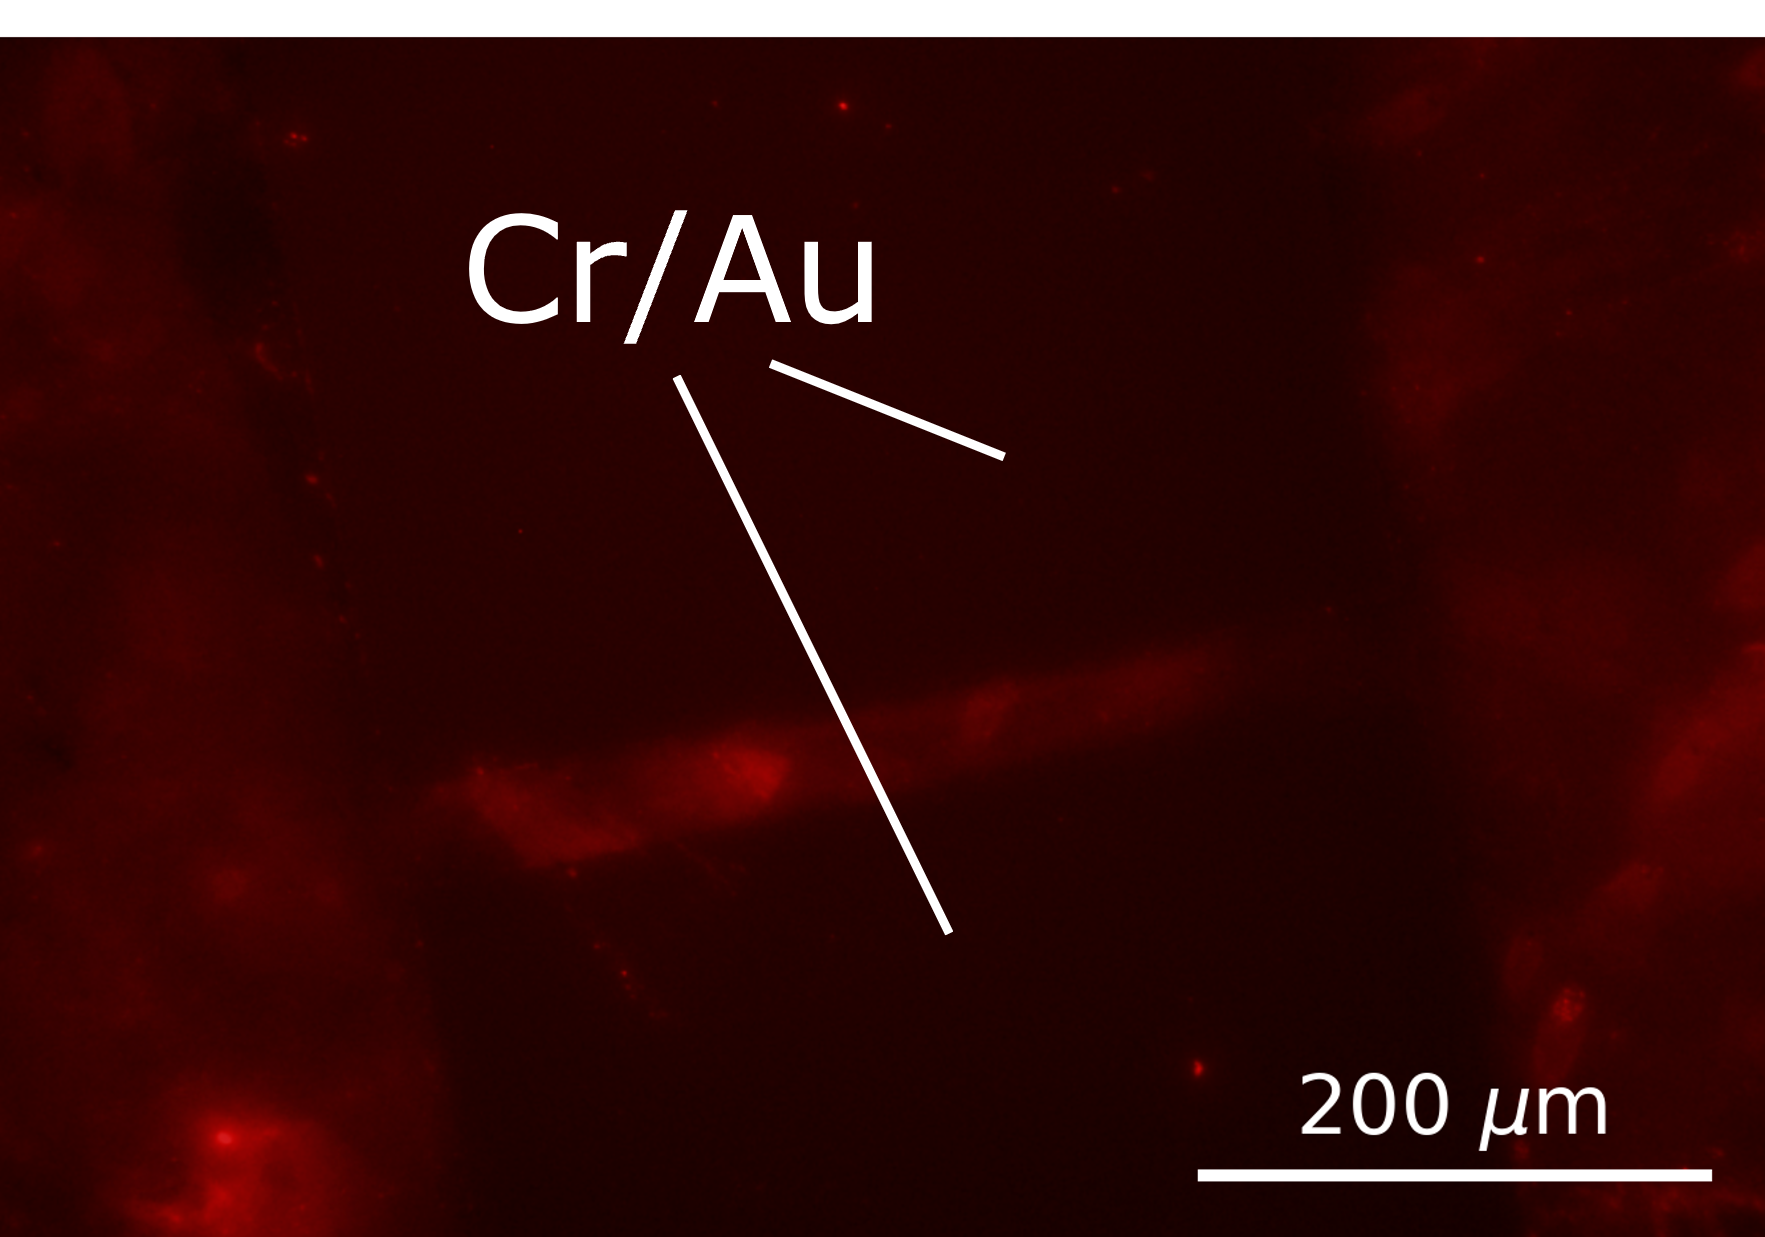
\includegraphics{figures/ch7/modified_hardbake_aptamer_ch3_mCherry_30sexposure_highcontrast_ISO200_12.6X.png}

}

}

\subcaption{\label{fig-aptamer-photoresist-4}}
\end{minipage}%

\caption{\label{fig-photoresist-contamination}A fluorescence image of a
SU8-encapsulated carbon nanotube device is shown in (a), while (b) shows
the same channel after modification with an solution of 1 mM
Pyrene-PEG-FITC. A 0.35 s exposure time and FITC filter were used for
(a)-(b). The fluorescence image in (c) shows an unencapsulated channel,
while (d) shows the same channel after Cy3-tagged aptamer exposure. A 10
s exposure time and mCherry filter were used for (c)-(d). The
fluorescence images in (e) and (f) show devices pre-coated with a thin
layer of photoresist then submerged in Cy3-tagged aptamer, where the
device in (f) was hardbaked before aptamer exposure. An mCherry filter
and 30 s exposure time were used for for (e)-(f).}

\end{figure}

An functionalisation issue quickly encountered when characterising
pyrene-PEG-FITC (PPF) interaction with sensing channels via fluorescence
microscopy was an unwanted secondary interaction between the linker and
residual photoresist. Figure~\ref{fig-350ms-SU8} and
Figure~\ref{fig-350ms-SU8-FITC} are fluorescence images of SU8
encapsulation (using the pre-2023 mask) before and after being exposed
to PPF. Despite the same microscope settings being used to take the
images (filter, ISO, contrast, exposure time), the SU8 exposed to PPF
appears much brighter than the pristine SU8. This result indicates that
the linker appears to have an extensive interaction with the photoresist
via an unknown mechanism. No fluorescence is seen from the device
channel. The length of exposure time required to see fluorescence from
the modified channel would lead to fluorescence from the modified linker
attached to the photoresist \(-\) as well as the photoresist itself
\(-\) flooding the image with light. Therefore, it is not clear whether
the carbon nanotubes have been functionalised with the dye-modified
linker. However, out of caution we can assume that the presence of this
secondary interaction is not desirable.

A similar interaction was seen between AZ\(^\circledR\) 1518 photoresist
and fluorescent-tagged, amine-terminated aptamer. An unencapsulated
carbon nanotube network device, fabricated using the pre-June 2022
process outlined in \textbf{?@sec-fabrication}, was incubated with 500
nM Cy3-tagged aptamer in Tris buffer at 4°C overnight. The aptamer was
first denatured by heating in a water bath at 95°C for 5 minutes then
cooling in an ice bath for 10 minutes before use.

Figure~\ref{fig-aptamer-photoresist-1} and
Figure~\ref{fig-aptamer-photoresist-2} are fluorescence images of the
device channel region before and after exposure to aptamer. A thick red
ring is visible around the electrodes after functionalisation, despite
no PBASE being used to tether the amine-terminated aptamer. It appears
that these bright patches correspond to patches of residual photoresist
which have not been completely removed from the carbon nanotube square
by the development process. These patches have then interacted with the
aptamer, causing them to appear bright under the fluorescence
microscope. Beyond potentially interfering with functionalisation,
photoresist residue blocking a device channel will prevent interaction
with the buffer and prevent sensing.

To test whether residual resist could be prevented from interacting with
aptamer by crosslinking the resist, two unencapsulated devices were
prepared as follows. Devices were first spincoated with AZ\(^\circledR\)
1518 in the manner described in \textbf{?@sec-fabrication}. Next, the
majority of resist was removed by soaking the device in acetone for 1
minute. This process left a thin coating of photoresist on the devices.
One of these devices was then hardbaked at 200°C for 1 hour. Both
devices were subsequently functionalised in the following manner:

\begin{enumerate}
\def\labelenumi{\arabic{enumi}.}
\item
  Unencapsulated device was submerged in 1 mM PBASE in methanol solution
  for 1 hour.
\item
  The device was then rinsed with methanol and Tris buffer.
\item
  1 \(\mu\)M Cy3-tagged aptamer was denatured by heating in a water bath
  at 95°C for 5 minutes then cooling in an ice bath for 10 minutes
  before use.
\item
  The device was incubated with aptamer in Tris buffer at 4°C overnight.
\end{enumerate}

Fluorescence microscope images of channels from each device are shown in
Figure~\ref{fig-aptamer-photoresist-3} and
Figure~\ref{fig-aptamer-photoresist-4}, where the latter is the device
hardbaked before functionalisation. By comparing the two images, it is
apparent that hardbaking the AZ\(^\circledR\) 1518 photoresist
significantly reduces the amount of fluorescent aptamer attached to the
surface. This result is an indication that sufficient heating of the
photoresist can prevent it interacting with PBASE or amine-tagged
biological material. However, there is still some Cy3-tagged aptamer
fluorescence visible in Figure~\ref{fig-aptamer-photoresist-4}. It
appears that hardbaking has not completely prevented photoresist from
interacting with the aptamer. It is possible that heating from the
bottom of the device is insufficient to hardbake the photoresist layer
completely, an effect that would be amplified for the thick photoresist
layer on encapsulated devices. Therefore, from June 2023 onwards devices
were vacuum annealed for 1 hour at 150°C prior to functionalisation.
This approach was taken to ensure photoresist was heated from above as
well as below and made chemically inert across its surface.

This result demonstrates the use of fluorescence microscopy as a tool to
detect residue and test suitable residue elimination measures. Further
testing showed that performing a 1 minute flood exposure (for positive
resist only) then placing a device in AZ\(^\circledR\) 326 developer for
3 minutes was highly effective at removing photoresist residue. Both
these development and annealing techniques were used for all
functionalised devices in subsequent sections.

\hypertarget{sec-hydrophobicity}{%
\subsubsection{Hydrophobicity of Carbon Nanotubes and
Graphene}\label{sec-hydrophobicity}}

\begin{figure}

\begin{minipage}[t]{0.47\linewidth}

{\centering 

\raisebox{-\height}{

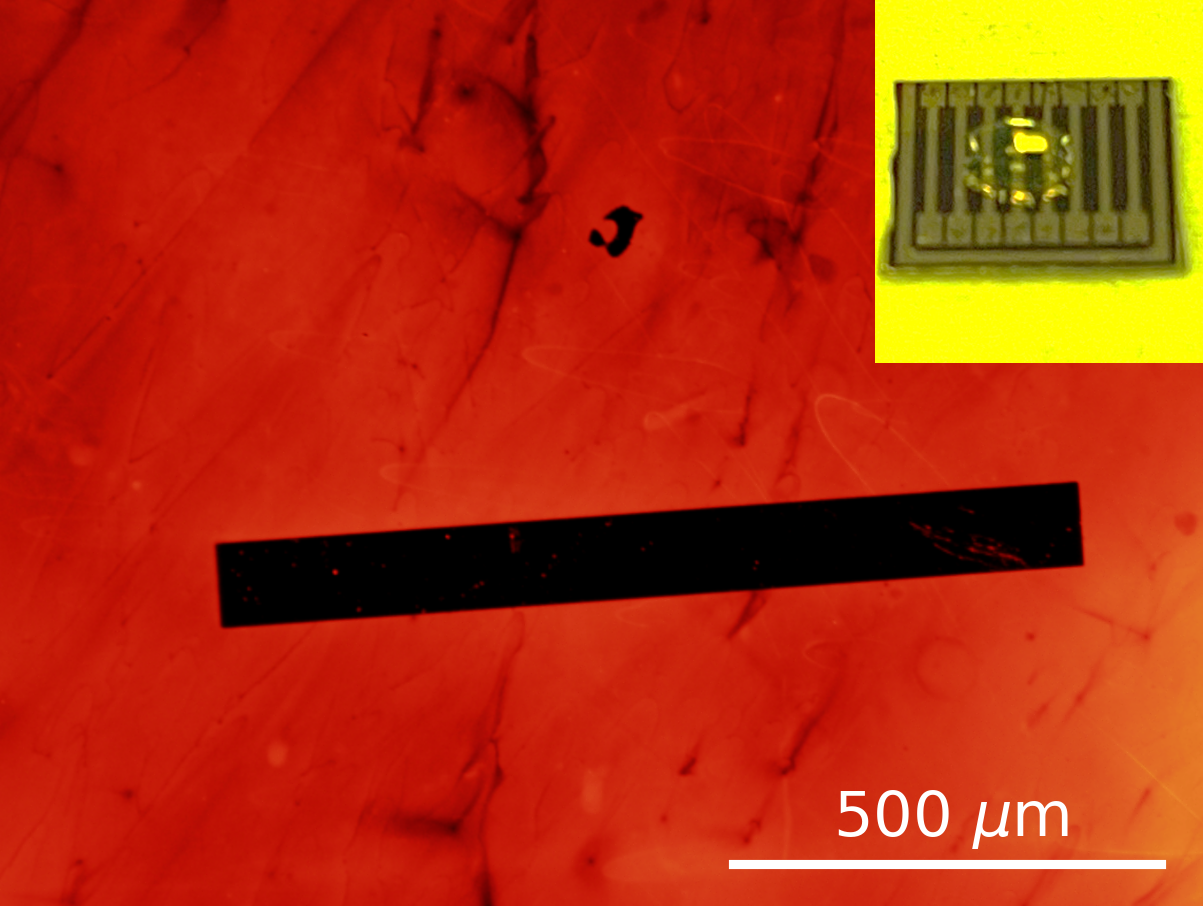
\includegraphics{figures/ch7/modified_NGW8D9_edgechannel_post10min50Cacetonerinse_221109.png}

}

}

\subcaption{\label{fig-no-attachment}}
\end{minipage}%
%
\begin{minipage}[t]{0.05\linewidth}

{\centering 

~

}

\end{minipage}%
%
\begin{minipage}[t]{0.47\linewidth}

{\centering 

\raisebox{-\height}{

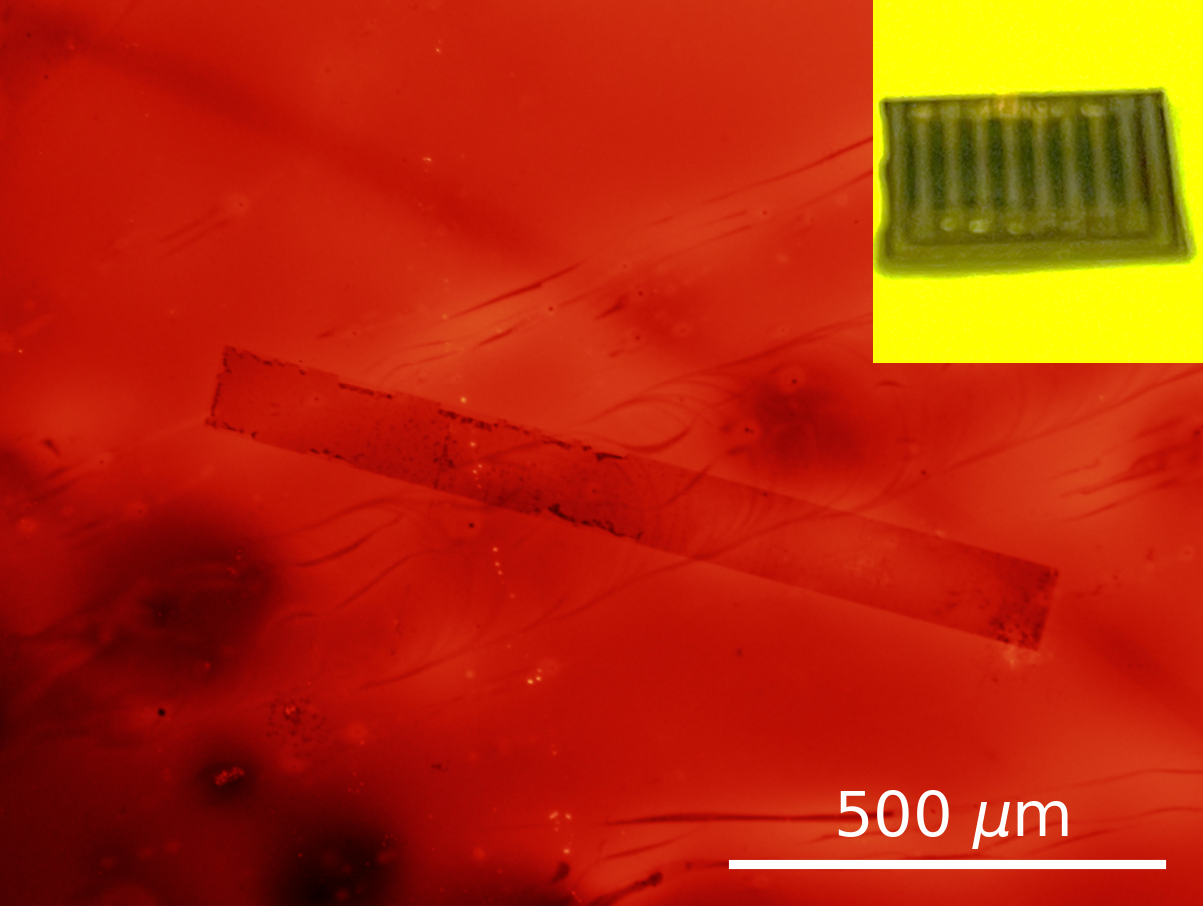
\includegraphics{figures/ch7/modified_NGW8D7_edgechannel_lowerexposuretime_221108.png}

}

}

\subcaption{\label{fig-attachment-post-plasma}}
\end{minipage}%

\caption{\label{fig-hydrophobicity}Fluorescence images of a 1000
\(\mu\)m \(\times\) 100 \(\mu\)m graphene channel after
functionalisation with 1 mM pyrene-PEG-rhodamine in 1XPBS. The graphene
film in (a) was not oxygen plasma cleaned before functionalisation,
while the graphene film in (b) was oxygen plasma cleaned at 5 W for 15 s
at 300 mTorr pressure immediately before functionalisation. Insets show
a 10 \(\mu\)L droplet placed on an unencapsulated carbon nanotube device
before (a) and after (b) the same oxygen plasma treatment procedure.
Images were taken using an Texas Red filter and a 1.8 s exposure time.}

\end{figure}

\begin{figure}

\begin{minipage}[t]{0.47\linewidth}

{\centering 

\raisebox{-\height}{

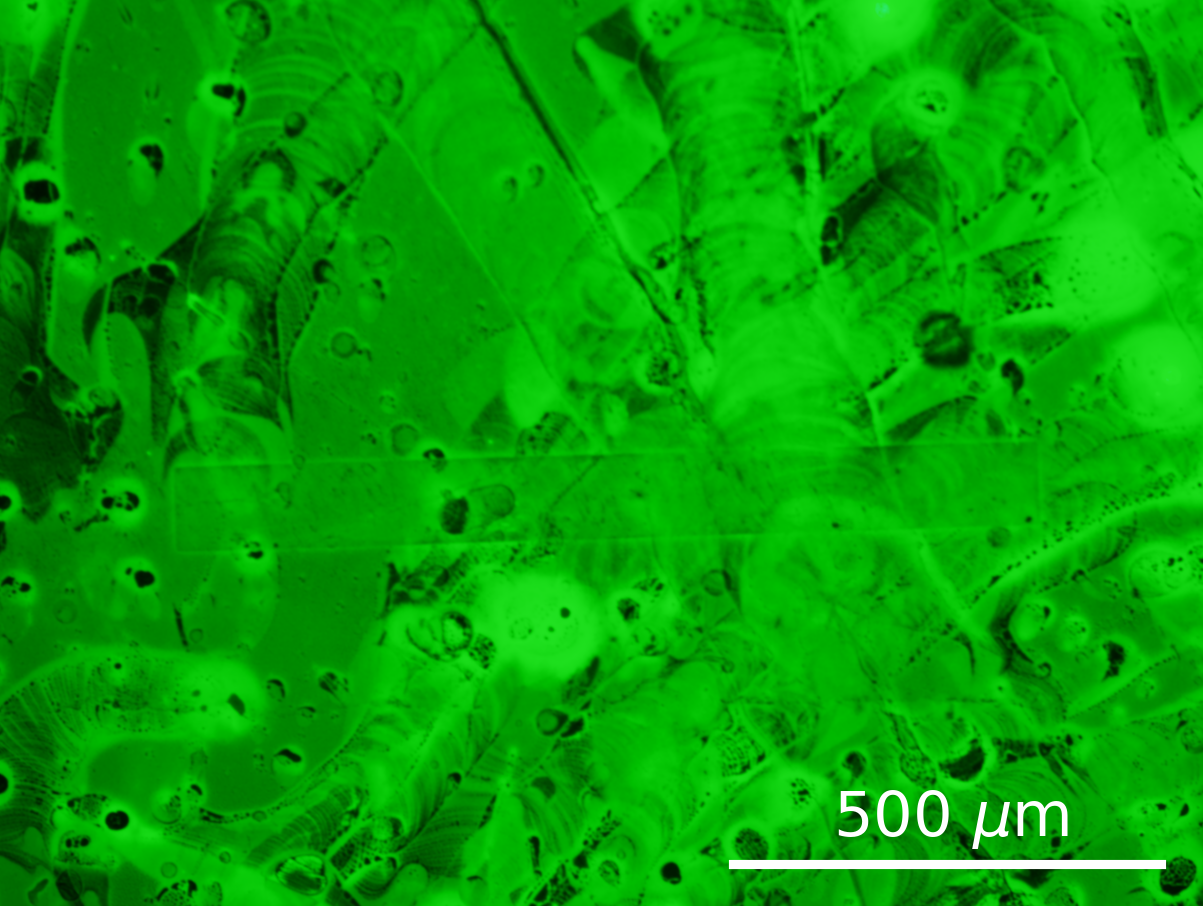
\includegraphics{figures/ch7/modified_NGW6D4_PyPEGFITC_channel2_1.6sexposure_10X_221122.png}

}

}

\subcaption{\label{fig-FITC-silicon-dioxide}}
\end{minipage}%
%
\begin{minipage}[t]{0.05\linewidth}

{\centering 

~

}

\end{minipage}%
%
\begin{minipage}[t]{0.47\linewidth}

{\centering 

\raisebox{-\height}{

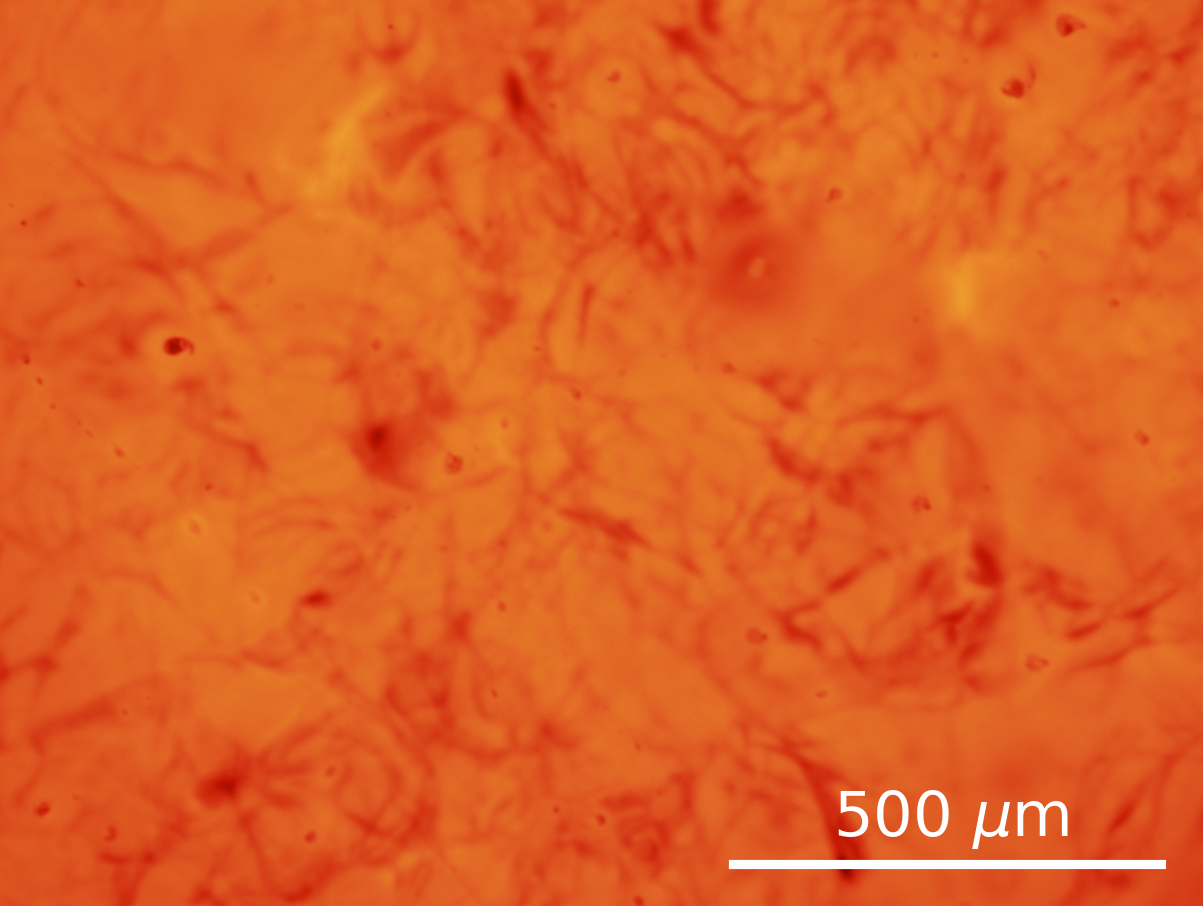
\includegraphics{figures/ch7/modified_SiO2_1mMPPR_2_221109.png}

}

}

\subcaption{\label{fig-rhodamine-silicon-dioxide}}
\end{minipage}%
\newline
\begin{minipage}[t]{0.47\linewidth}

{\centering 

\raisebox{-\height}{

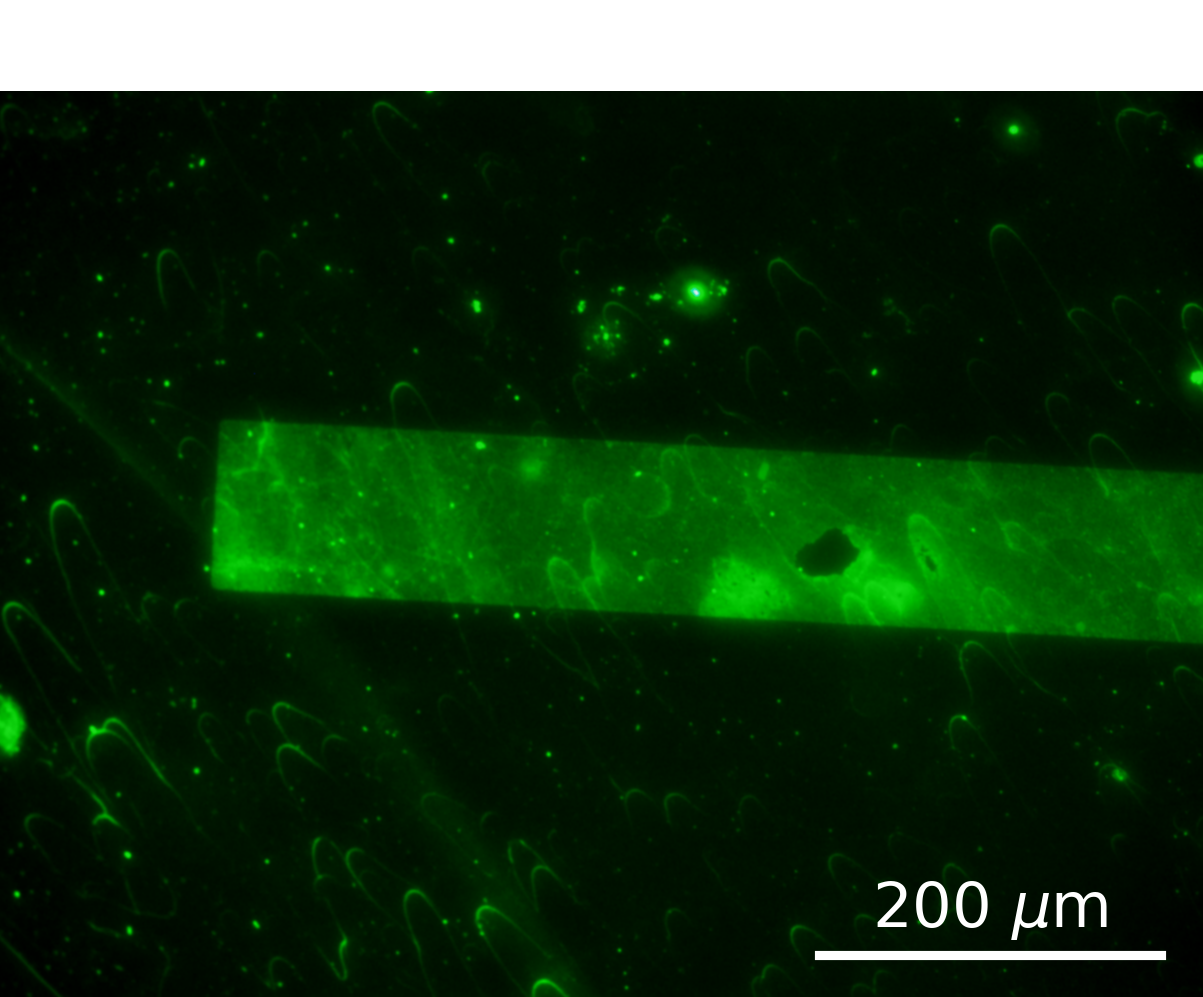
\includegraphics{figures/ch7/modified_NGW6D7_PyPEGFITC_channel3top_postmsurfclean_7.5sexposure_20X_221123.png}

}

}

\subcaption{\label{fig-PPF-PBS-20X}}
\end{minipage}%
%
\begin{minipage}[t]{0.05\linewidth}

{\centering 

~

}

\end{minipage}%
%
\begin{minipage}[t]{0.47\linewidth}

{\centering 

\raisebox{-\height}{

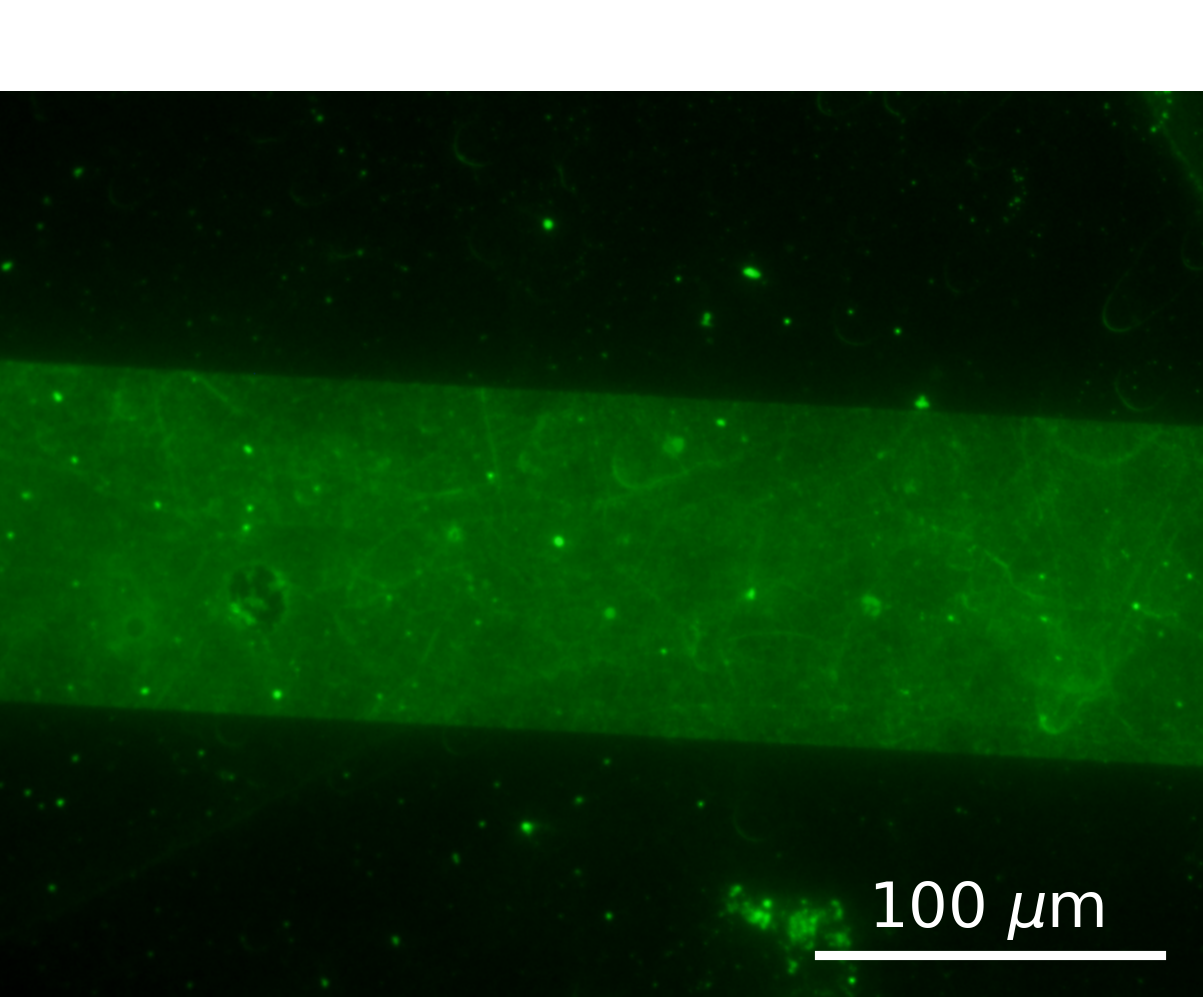
\includegraphics{figures/ch7/modified_NGW6D7_PyPEGFITC_channel1_postmsurfclean_7.75sexposure_40X_221123.png}

}

}

\subcaption{\label{fig-PPF-PBS-40X}}
\end{minipage}%

\caption{\label{fig-silicon-dioxide-interaction}The 1000 \(\mu\)m
\(\times\) 100 \(\mu\)m graphene film in image (a) was functionalised
with 1 mM pyrene-PEG-FITC in 1XPBS after oxygen plasma treatment, taken
using an FITC filter and a 1.6 s exposure time. (b) shows a silicon
dioxide surface which had never been exposed to carbon nanotubes,
graphene or photoresist after exposure to 1 mM pyrene-PEG-rhodamine in
1XPBS, taken using a Texas Red filter and a 1.8 s exposure time.
Graphene films on a substrate functionalised with 1 mM pyrene-PEG-FITC
in 1XPBS after oxygen plasma treatment then cleaned with m-CNT
dispersion surfactant (NanoIntegris) are shown in (c) and (d), where a
FITC filter was used, with 7.5 s and 7.75 s exposure times
respectively.}

\end{figure}

As PEGlyated linker dissolves well in aqueous solution, initial
fluorescence imaging focused on functionalising devices with these
linkers dissolved in 1XPBS. It was hoped that by keeping the device
channels in a pH-controlled environment, the channel surface would be
made more suitable for the attached receptors.
Figure~\ref{fig-no-attachment} shows a graphene film after exposure to
pyrene-PEG-rhodamine (PPR) in 1XPBS solution for 1 hour. The
pyrene-PEG-rhodamine has interacted with the silicon dioxide substrate
(discussed further in Section~\ref{sec-pyrene-interactions}) but not the
graphene film. The graphene has not attached to the pyrene or rhodamine
due to the highly hydrophobic graphene surface repelling the surrounding
solution, preventing \(\pi\)-stacking from occurring. The hydrophobicity
of the graphene surface is not intrinsic to graphene, but instead
results from a hydrocarbonaceous layer which forms on the channel
surface when exposed to air {[}@Ashraf2014{]}. A hydrophobic layer wiil
also form on carbon nanotube networks {[}@Stando2019; @Park2022{]}.
Treatment with oxygen plasma at 5 W for 15 s has previously been found
to remove this hydrocarbonaceous layer, restoring the intrinsic
hydrophilicity of graphene {[}@Shin2010{]}. Storing the graphene surface
in deionised water rather than air prevents the return of this
hydrocarbon layer {[}@Ashraf2014{]}. The use of a relatively low power
plasma ensures damage to the graphene layer is minimised.

Treatment of an unencapsulated carbon nanotube network device at 5 W for
15 s at 300 mTorr greatly reduced the contact angle of a water droplet
placed on the device surface, shown inset in
Figure~\ref{fig-hydrophobicity} before and after plasma treatment. A
graphene film was then functionalised with pyrene-PEG-rhodamine in 1XPBS
in the same manner as for the film in Figure~\ref{fig-no-attachment},
except with the same plasma treatment performed on the film less than 1
minute before functionalisation. The result is shown in
Figure~\ref{fig-attachment-post-plasma}. The graphene now appears to
interact with the pyrene-PEG-rhodamine. These results both indicate that
the plasma treatment is increasing the hydrophilicity of the device
surface, improving the ability of pyrene-PEG-rhodamine to \(\pi\)-stack
with graphene. The disadvantage of this procedure is that the plasma
cleaning introduces defects to the graphene surface which may be
undesirable for device electrical behaviour. Furthermore, it was often
found that devices functionalised in this manner had their conductance
drop significantly after functionalisation, even though plasma treatment
itself did not significantly alter device conductance. Solvent was
therefore used for the initial linker functionalisation in
Section~\ref{sec-linker-receptor-attachment}, as it did not require a
plasma cleaning step for successful attachment.

\hypertarget{sec-pyrene-interactions}{%
\subsubsection{Substrate Interaction with Linker
Molecules}\label{sec-pyrene-interactions}}

Another issue that arose when verifying surface functionalisation was
the interaction between pyrene linker and the silicon dioxide substrate.
This interaction meant it was difficult to discern whether the pyrene
group was interacting in a specific manner with the channel film. It was
confirmed that pyrene-PEG was interacting with silicon dioxide, rather
than residual photoresist or nanomaterial, by performing a
pyrene-PEG-rhodamine functionalisation on pristine silicon dioxide, as
shown in Figure~\ref{fig-rhodamine-silicon-dioxide}. The PEGlyated
linker supplier suggested that the surface should be thoroughly rinsed
with surfactant to remove weakly-bound pyrene-PEG-FITC attached to the
silicon dioxide, while preserving the pyrene-PEG-FITC strongly attached
via \(\pi\)-stacking to the graphene or carbon nanotube film
{[}@CreativePEGworks2022{]}. The following process was then used to
remove pyrene-PEG-FITC from the silicon dioxide: the film was rinsed
with DI water for 30 s, then placed in m-CNT dispersion solution
(NanoIntegris) for 5 minutes at 70°C while agitating with a pipette, and
finally rinsed with DI water, ethanol, acetone, IPA and nitrogen dried.
The results of this thorough cleaning process are shown in
Figure~\ref{fig-PPF-PBS-20X} and Figure~\ref{fig-PPF-PBS-40X}. The
majority of pyrene-PEG-FITC was removed in regions with no graphene, but
remained where graphene was present, indicating specific,
\(\pi\)-stacking interaction took place between the pyrene-PEG-FITC and
graphene. However, this surfactant rinse step was not used when
performing functionalisation with biological materials, to prevent
damage to the lipid membranes used.

\hypertarget{sec-coffee-ring}{%
\subsubsection{Coffee-Ring Effect}\label{sec-coffee-ring}}

\begin{figure}

\begin{minipage}[t]{0.47\linewidth}

{\centering 

\raisebox{-\height}{

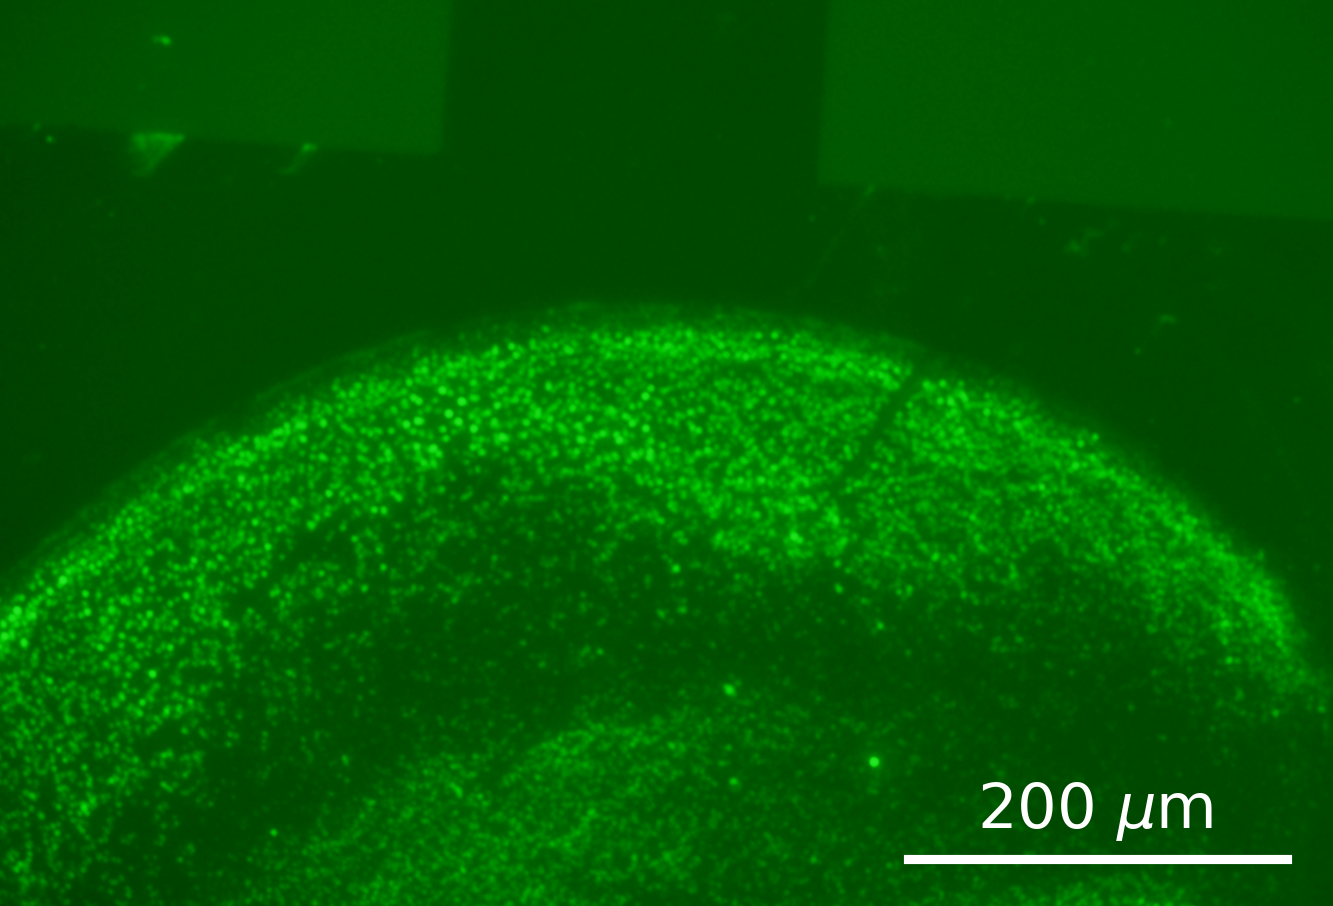
\includegraphics{figures/ch7/modified_GFPNi2+1_5sexposure_12.6X_mediumcontrast_18_230324.png}

}

}

\subcaption{\label{fig-GFP-coffee-ring-1}}
\end{minipage}%
%
\begin{minipage}[t]{0.05\linewidth}

{\centering 

~

}

\end{minipage}%
%
\begin{minipage}[t]{0.47\linewidth}

{\centering 

\raisebox{-\height}{

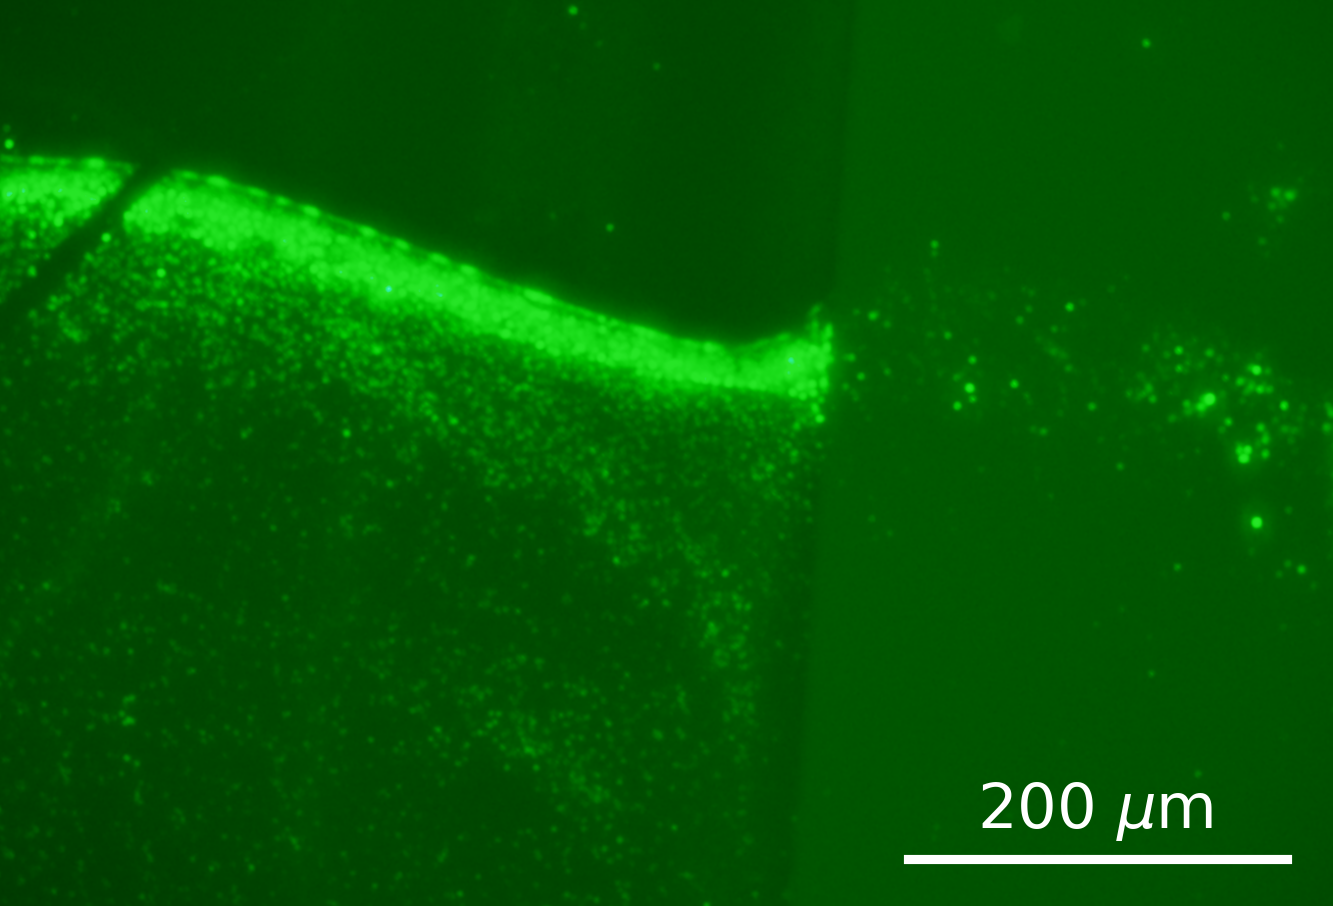
\includegraphics{figures/ch7/modified_GFPNi2+1_5sexposure_12.6X_mediumcontrast_20_230324.png}

}

}

\subcaption{\label{fig-GFP-coffee-ring-2}}
\end{minipage}%

\caption{\label{fig-GFP-coffee-ring}Both (a) and (b) show a build-up of
his-tag GFP at the edges of the droplet region where pyrene-PEG-NTA had
been present, taken using an GFP filter and a 5 s exposure time. On the
right hand side of (b), no his-tag GFP is visible on the metal
electrode, as no pyrene-PEG attaches to the metal electrodes.}

\end{figure}

From Table~\ref{tbl-pbase-functionalisation}, full device submersion
appears to be the most common approach for functionalisation with
solution containing linker molecules like PBASE. However, some groups
placed small droplets of solution onto the device channels when
functionalisation, and this approach was tested as part of the
fluorescence verification work. For functionalisation with his-tagged
green fluorescent protein, after plasma cleaning at 5 W for 15 s at 300
mTorr, a 4 \(\mu\)L droplet of 100\(\mu\)M pyrene-PEG-NTA in 1XPBS was
placed on each graphene device channel and left covered in a humid
environment for 15 minutes. The device was then rinsed with 1XPBS,
submerged in 10 mM NiSO\(_4\) in 1XPBS for 1 hour, rinsed in 1XPBS, then
submerged in 10 mL of 100 ng/mL his-tag GFP solution (Thermofisher)
overnight. Fluorescence microscope imaging showed that a ring of
biomaterial would build up around the outer edge of regions where
pyrene-PEG-NTA had been present, as seen in
Figure~\ref{fig-GFP-coffee-ring}.

It appears this is a result of the his-tag GFP attaching to a dense
region of pyrene-PEG-NTA at the edge of the functionalisation droplet.
This accretion of pyrene-PEG-NTA at the edge of the droplet is a result
of the coffee-ring effect, where the evaporation of the droplet leads to
transport of particles to the droplet edges via capillary flow
{[}@Deegan1997; @Shimobayashi2018{]}. As this gradient in surface
coverage of attached proteins has unknown consequences for sensing, in
subsequent sections devices were functionalised with PBASE or
pyrene-PEG-NTA by submerging them in solution instead of dropcasting.

\hypertarget{sec-linker-receptor-attachment}{%
\subsection{Verifying Linker-OR Nanodisc Attachment with Fluorescence
Microscopy}\label{sec-linker-receptor-attachment}}

To verify the formation of amide (or imide) bonds between PBASE and the
odorant receptors (ORs) contained within nanodiscs, a fluorescent
biomarker was directly attached to the odorant receptors for detection
with fluorescence microscopy. The biomarker used was the \emph{Aequorea
Victoria} green fluorescent protein (GFP). As far as I know, this is the
first time fluorescence has been used to verify the successful
attachment of odorant receptor nanodiscs to a carbon nanotube network.

\begin{figure}

\begin{minipage}[t]{0.47\linewidth}

{\centering 

\raisebox{-\height}{

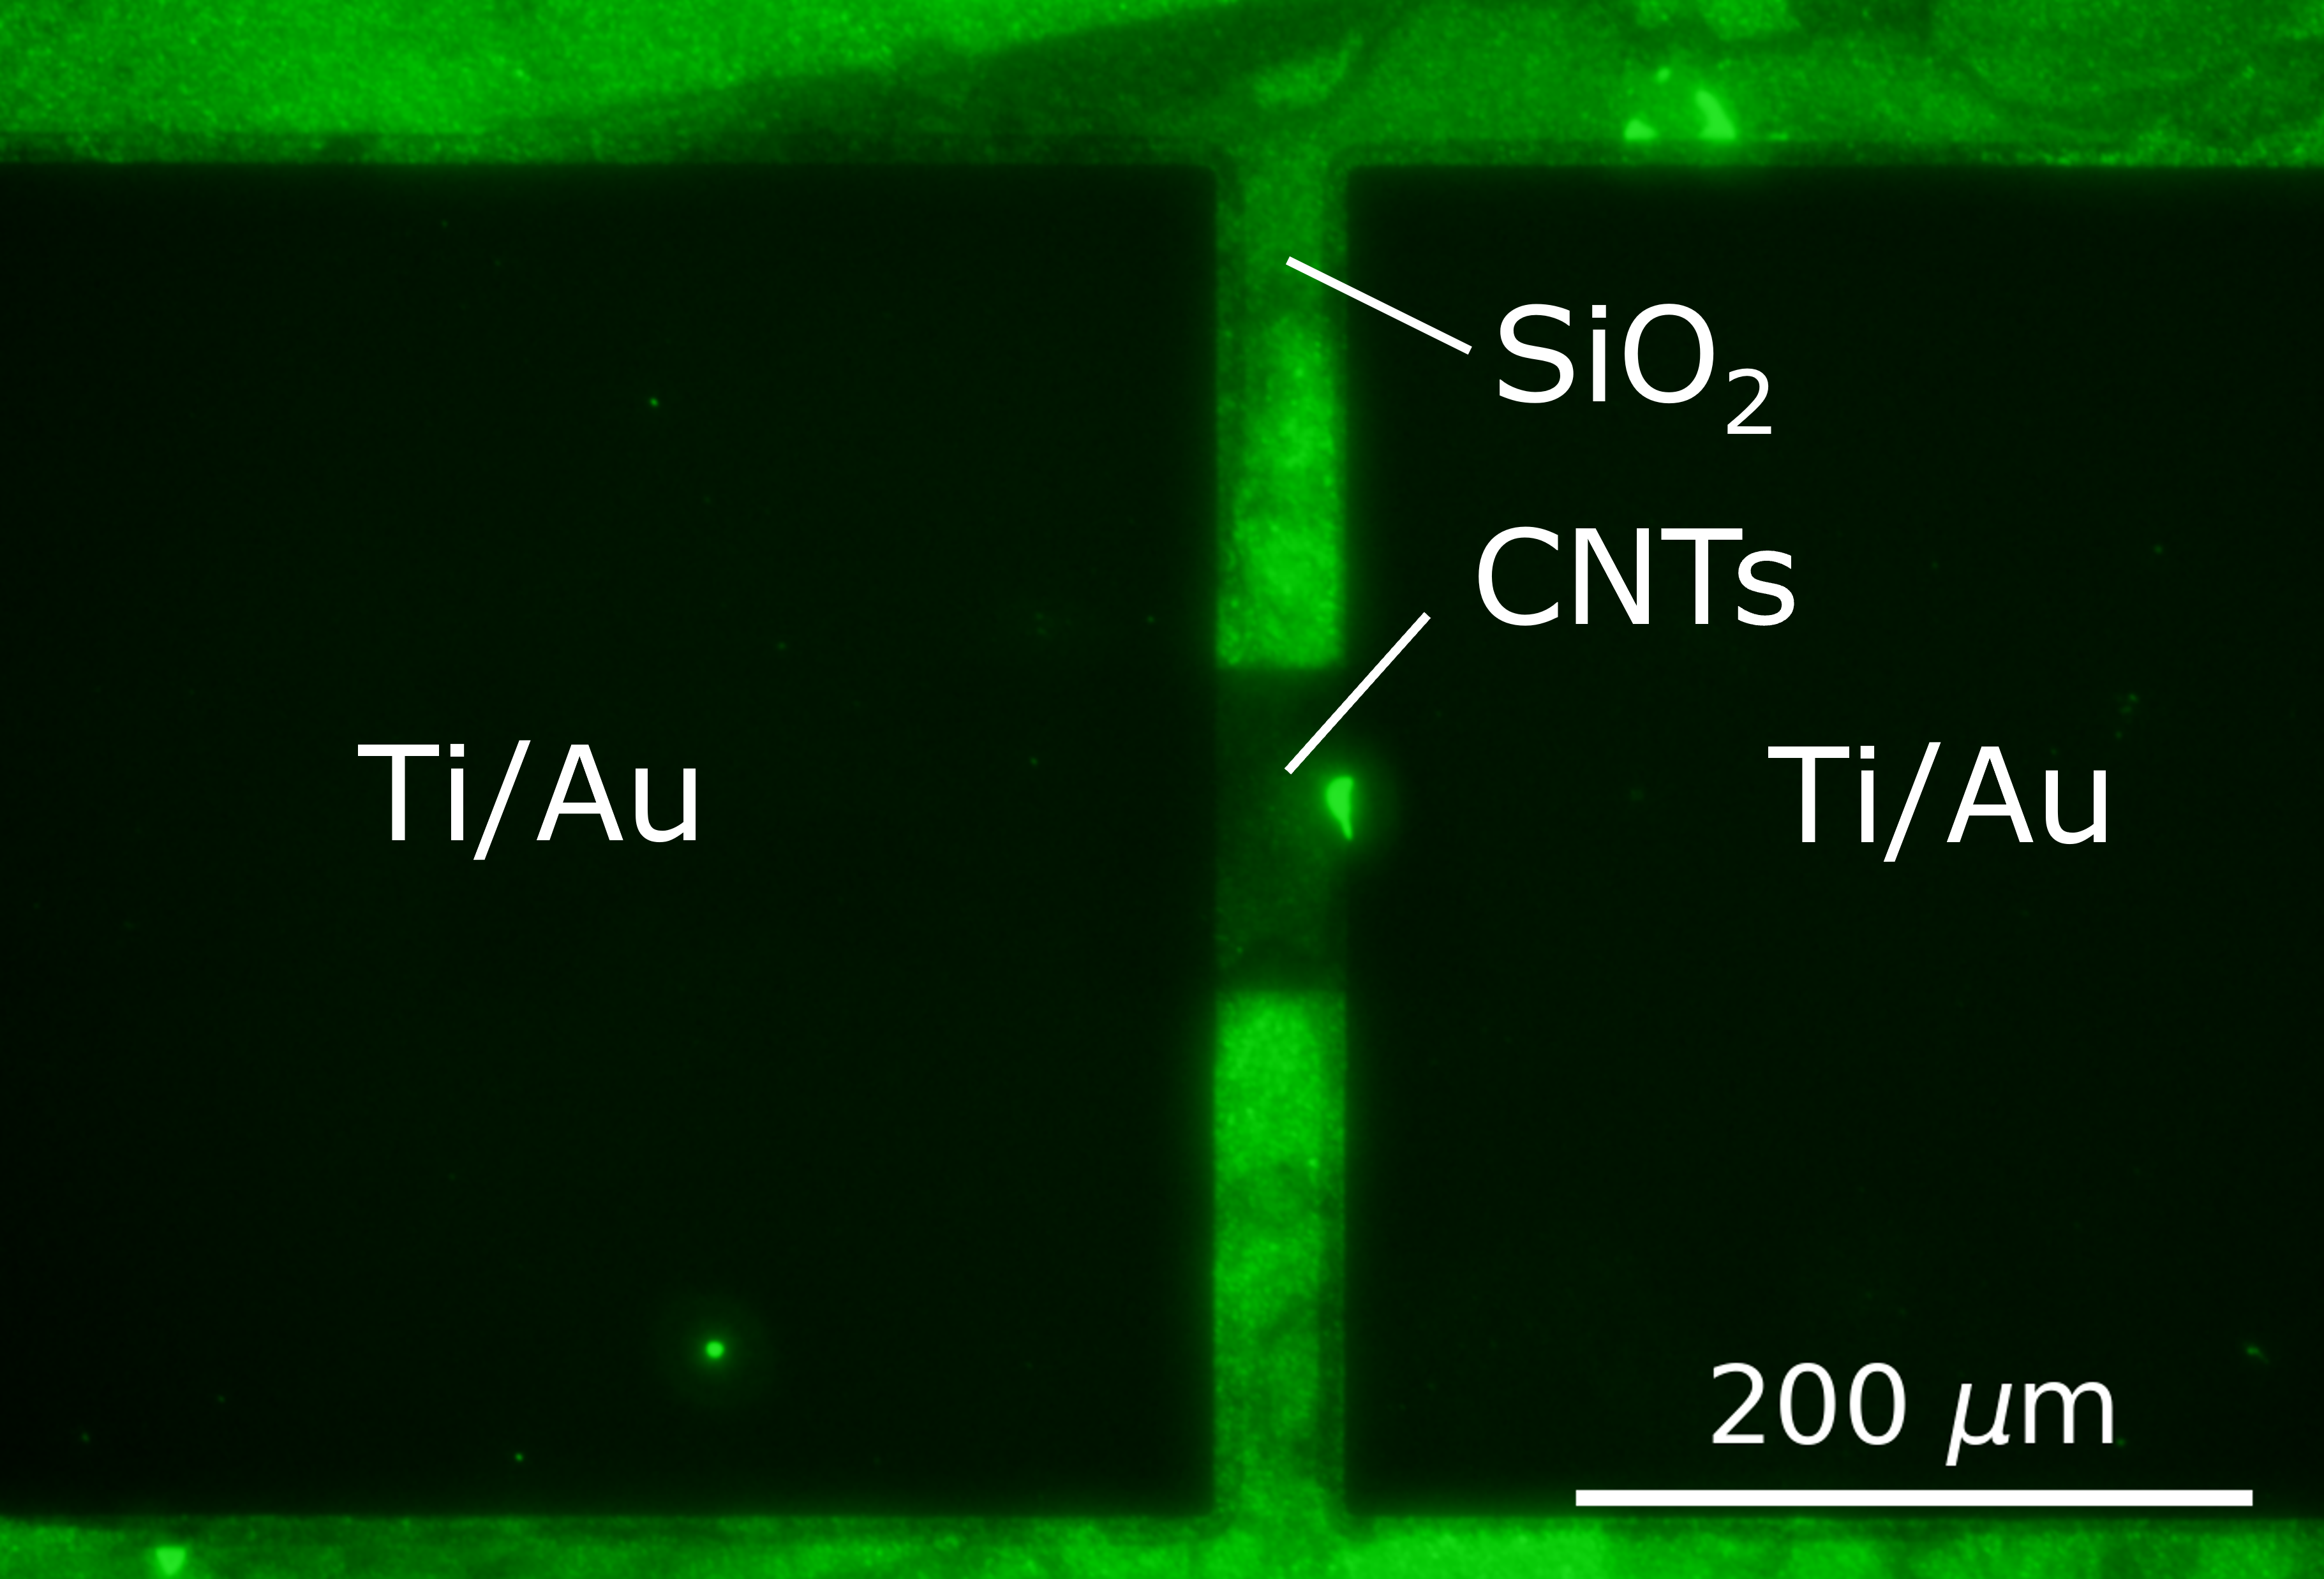
\includegraphics{figures/ch7/modified_GFPOR_10sexposure_20X_mediumcontrast_ch6_240208.png}

}

}

\subcaption{\label{fig-GFP-OR-ch6-zoom}}
\end{minipage}%
%
\begin{minipage}[t]{0.05\linewidth}

{\centering 

~

}

\end{minipage}%
%
\begin{minipage}[t]{0.47\linewidth}

{\centering 

\raisebox{-\height}{

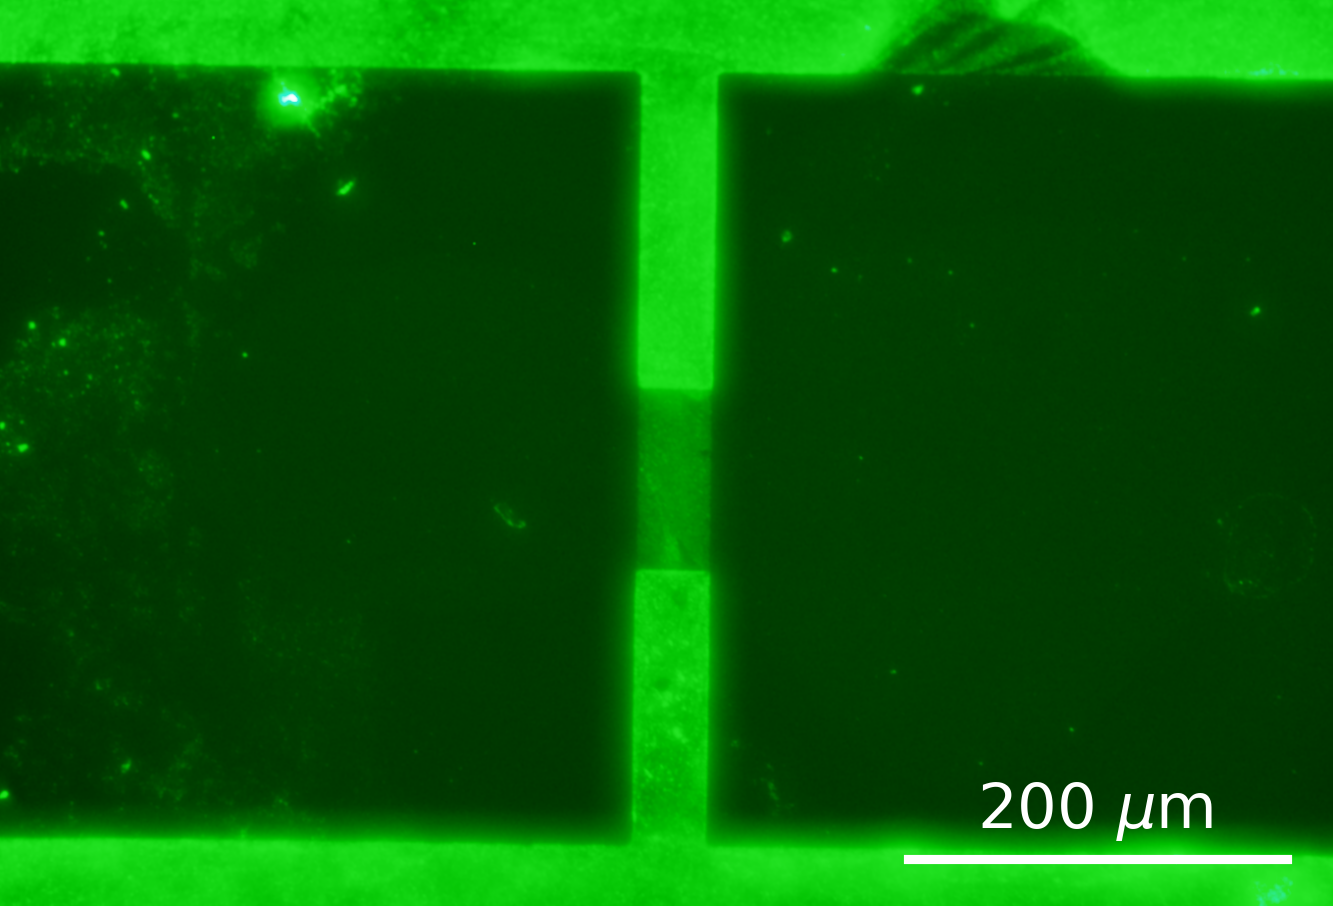
\includegraphics{figures/ch7/modified_GFPOR_PBASE_10sexposure_20X_mediumcontrast_ch1_231019_2.png}

}

}

\subcaption{\label{fig-PBASE-GFP-OR-ch1-zoom}}
\end{minipage}%
\newline
\begin{minipage}[t]{0.47\linewidth}

{\centering 

\raisebox{-\height}{

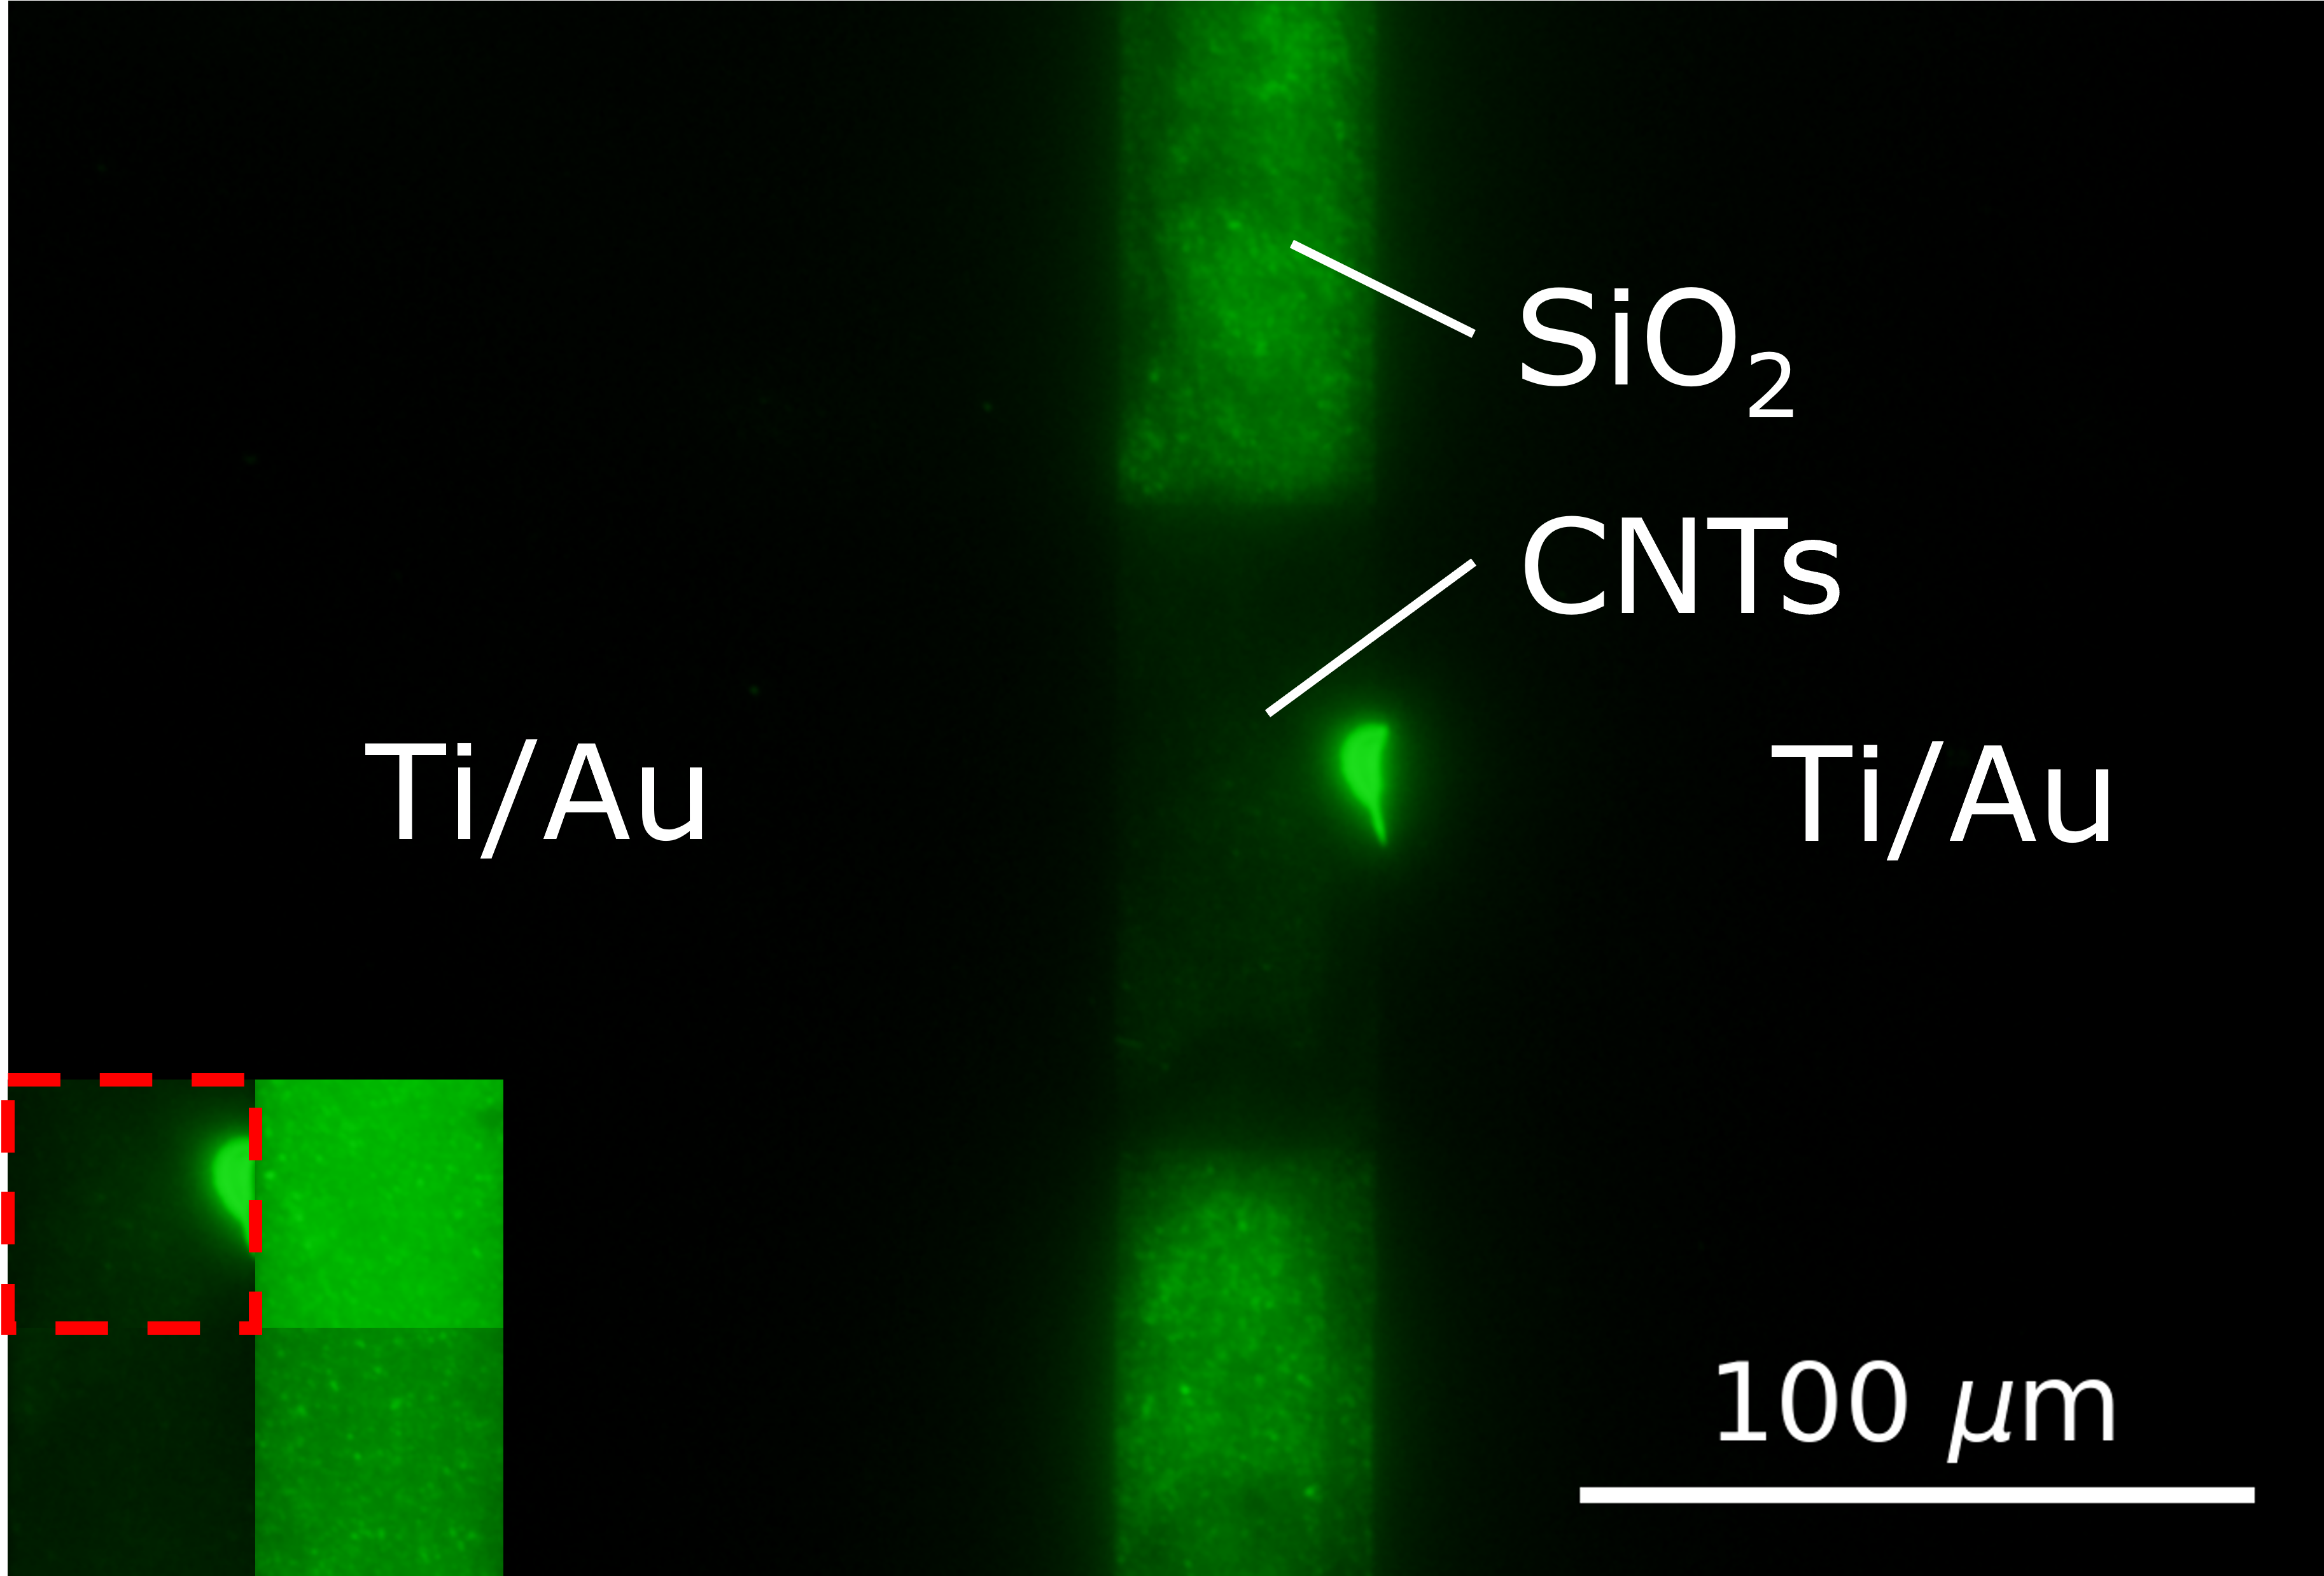
\includegraphics{figures/ch7/modified_GFPOR_10sexposure_40X_mediumcontrast_ch6_240208.png}

}

}

\subcaption{\label{fig-GFP-OR-ch6}}
\end{minipage}%
%
\begin{minipage}[t]{0.05\linewidth}

{\centering 

~

}

\end{minipage}%
%
\begin{minipage}[t]{0.47\linewidth}

{\centering 

\raisebox{-\height}{

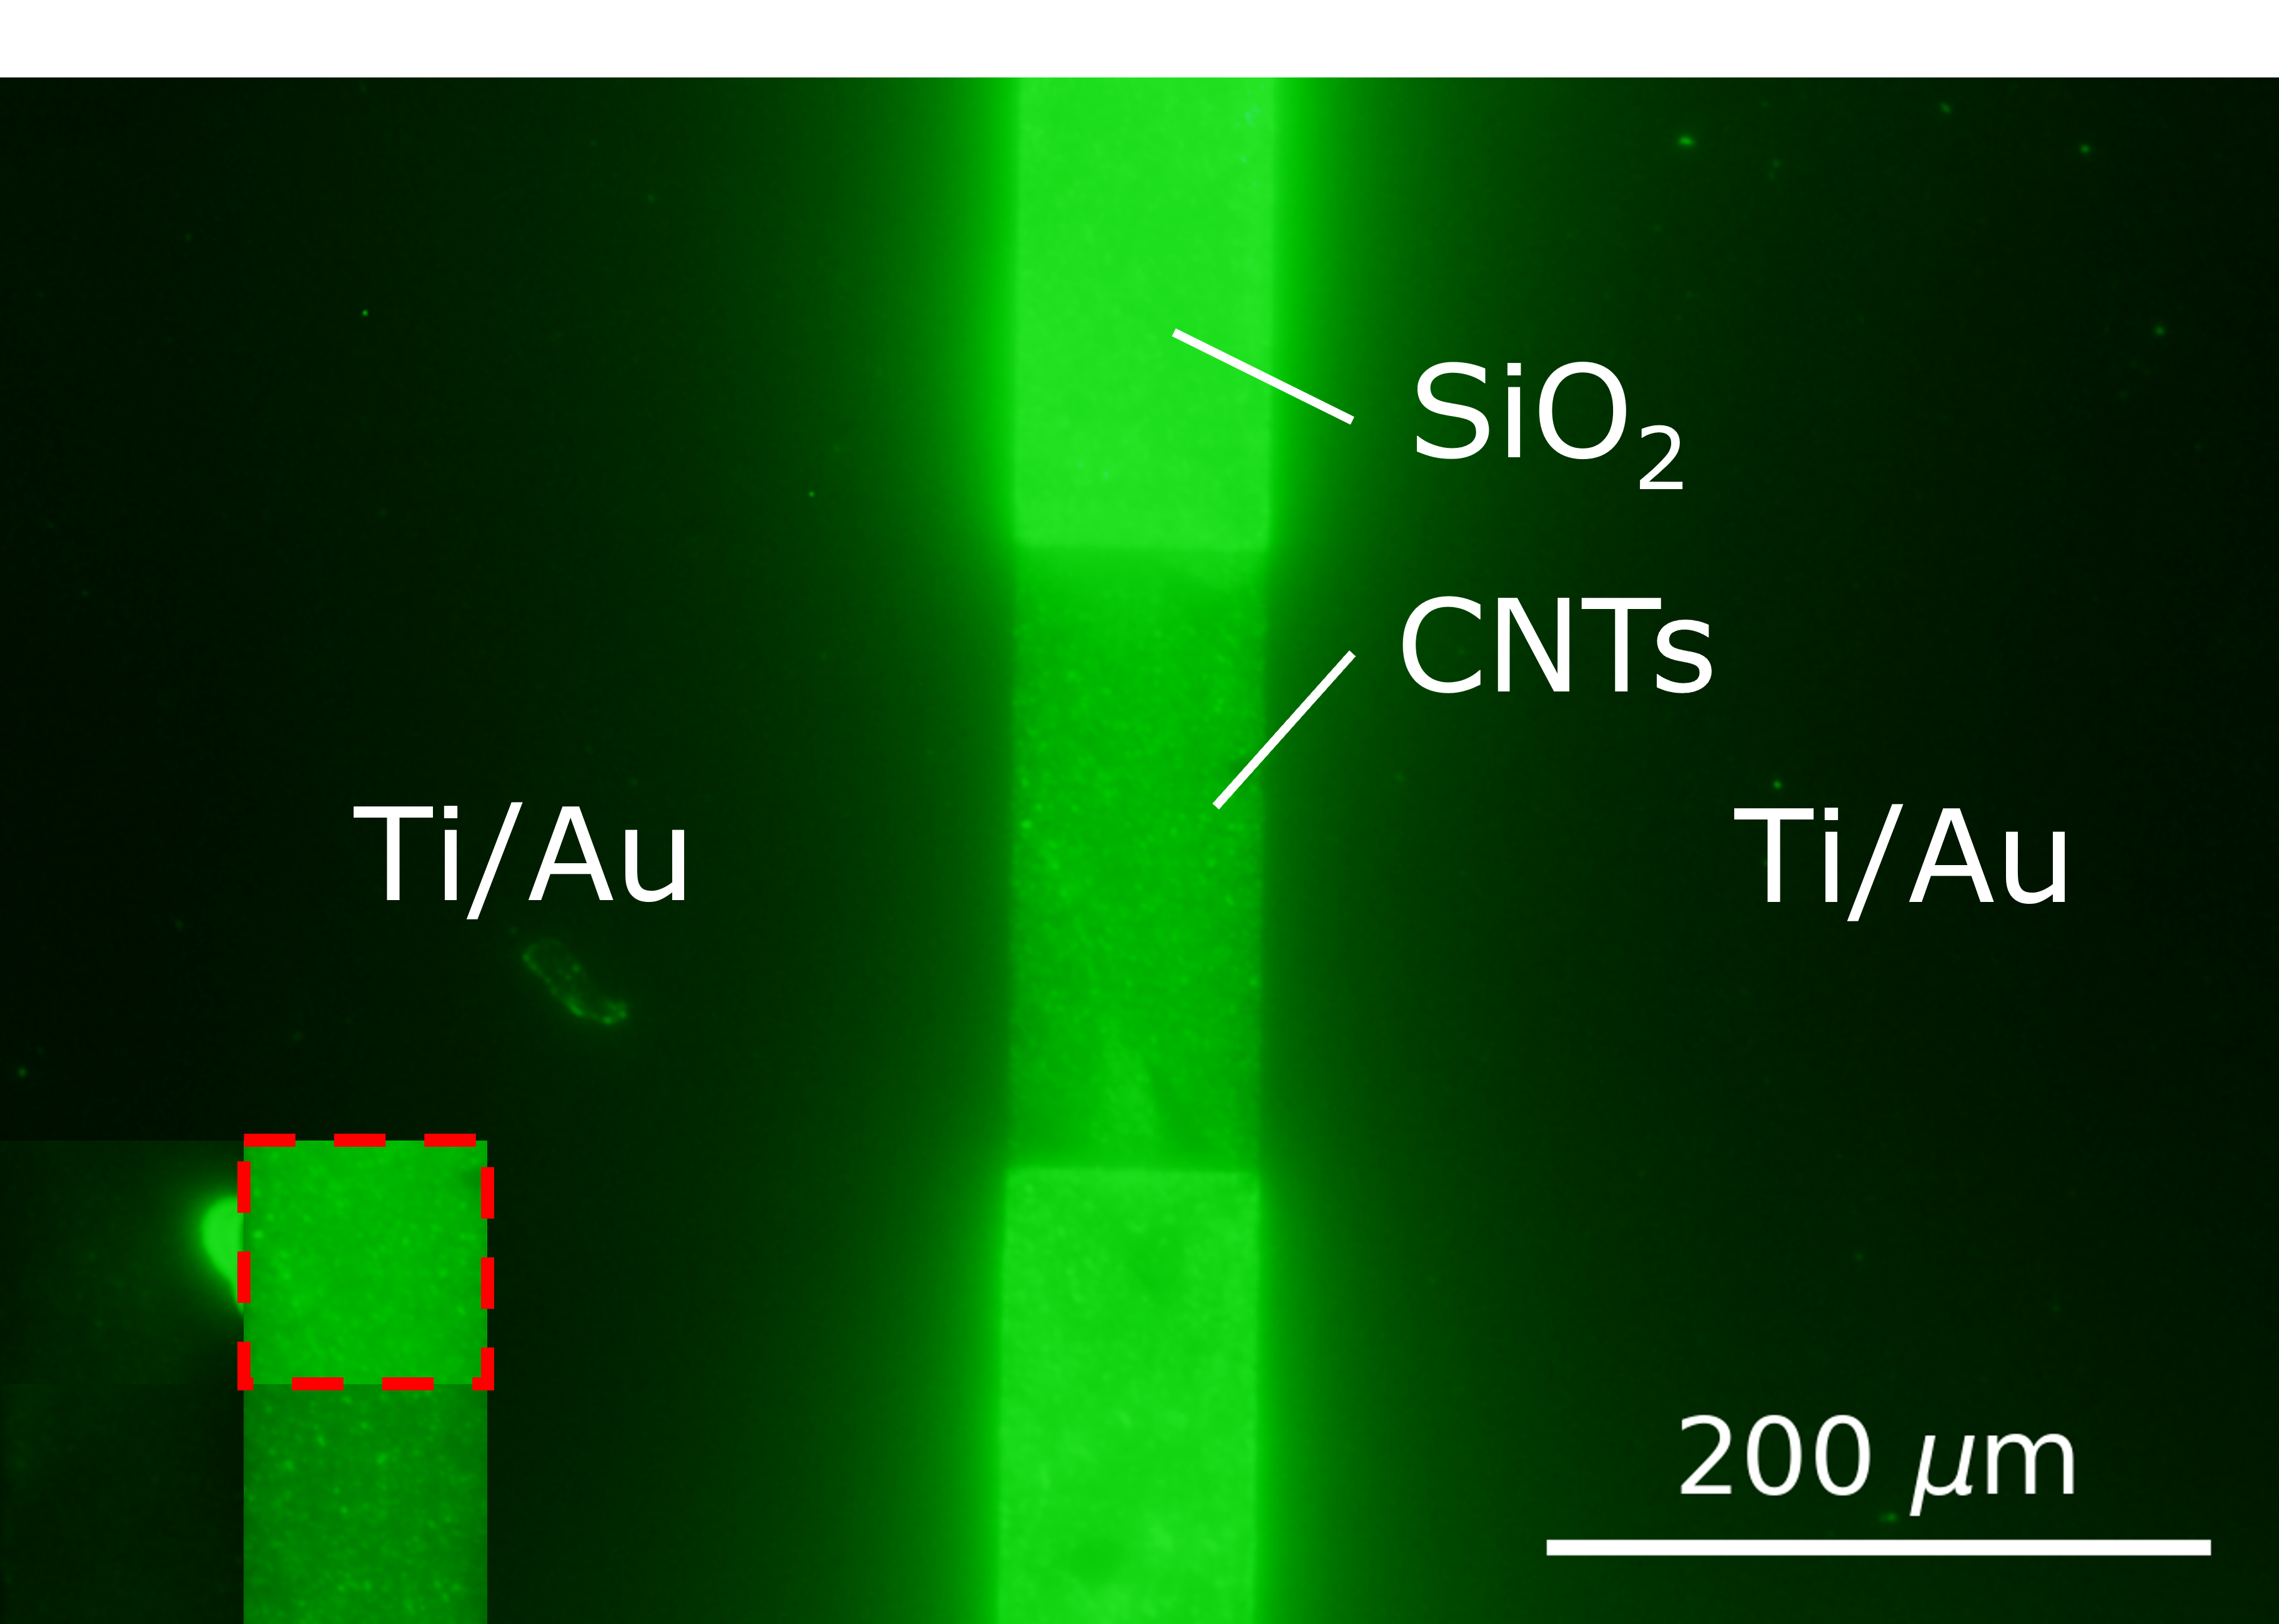
\includegraphics{figures/ch7/modified_GFPOR_PBASE_10sexposure_40X_mediumcontrast_ch1_231019_2.png}

}

}

\subcaption{\label{fig-PBASE-GFP-OR-ch1}}
\end{minipage}%
\newline
\begin{minipage}[t]{0.47\linewidth}

{\centering 

\raisebox{-\height}{

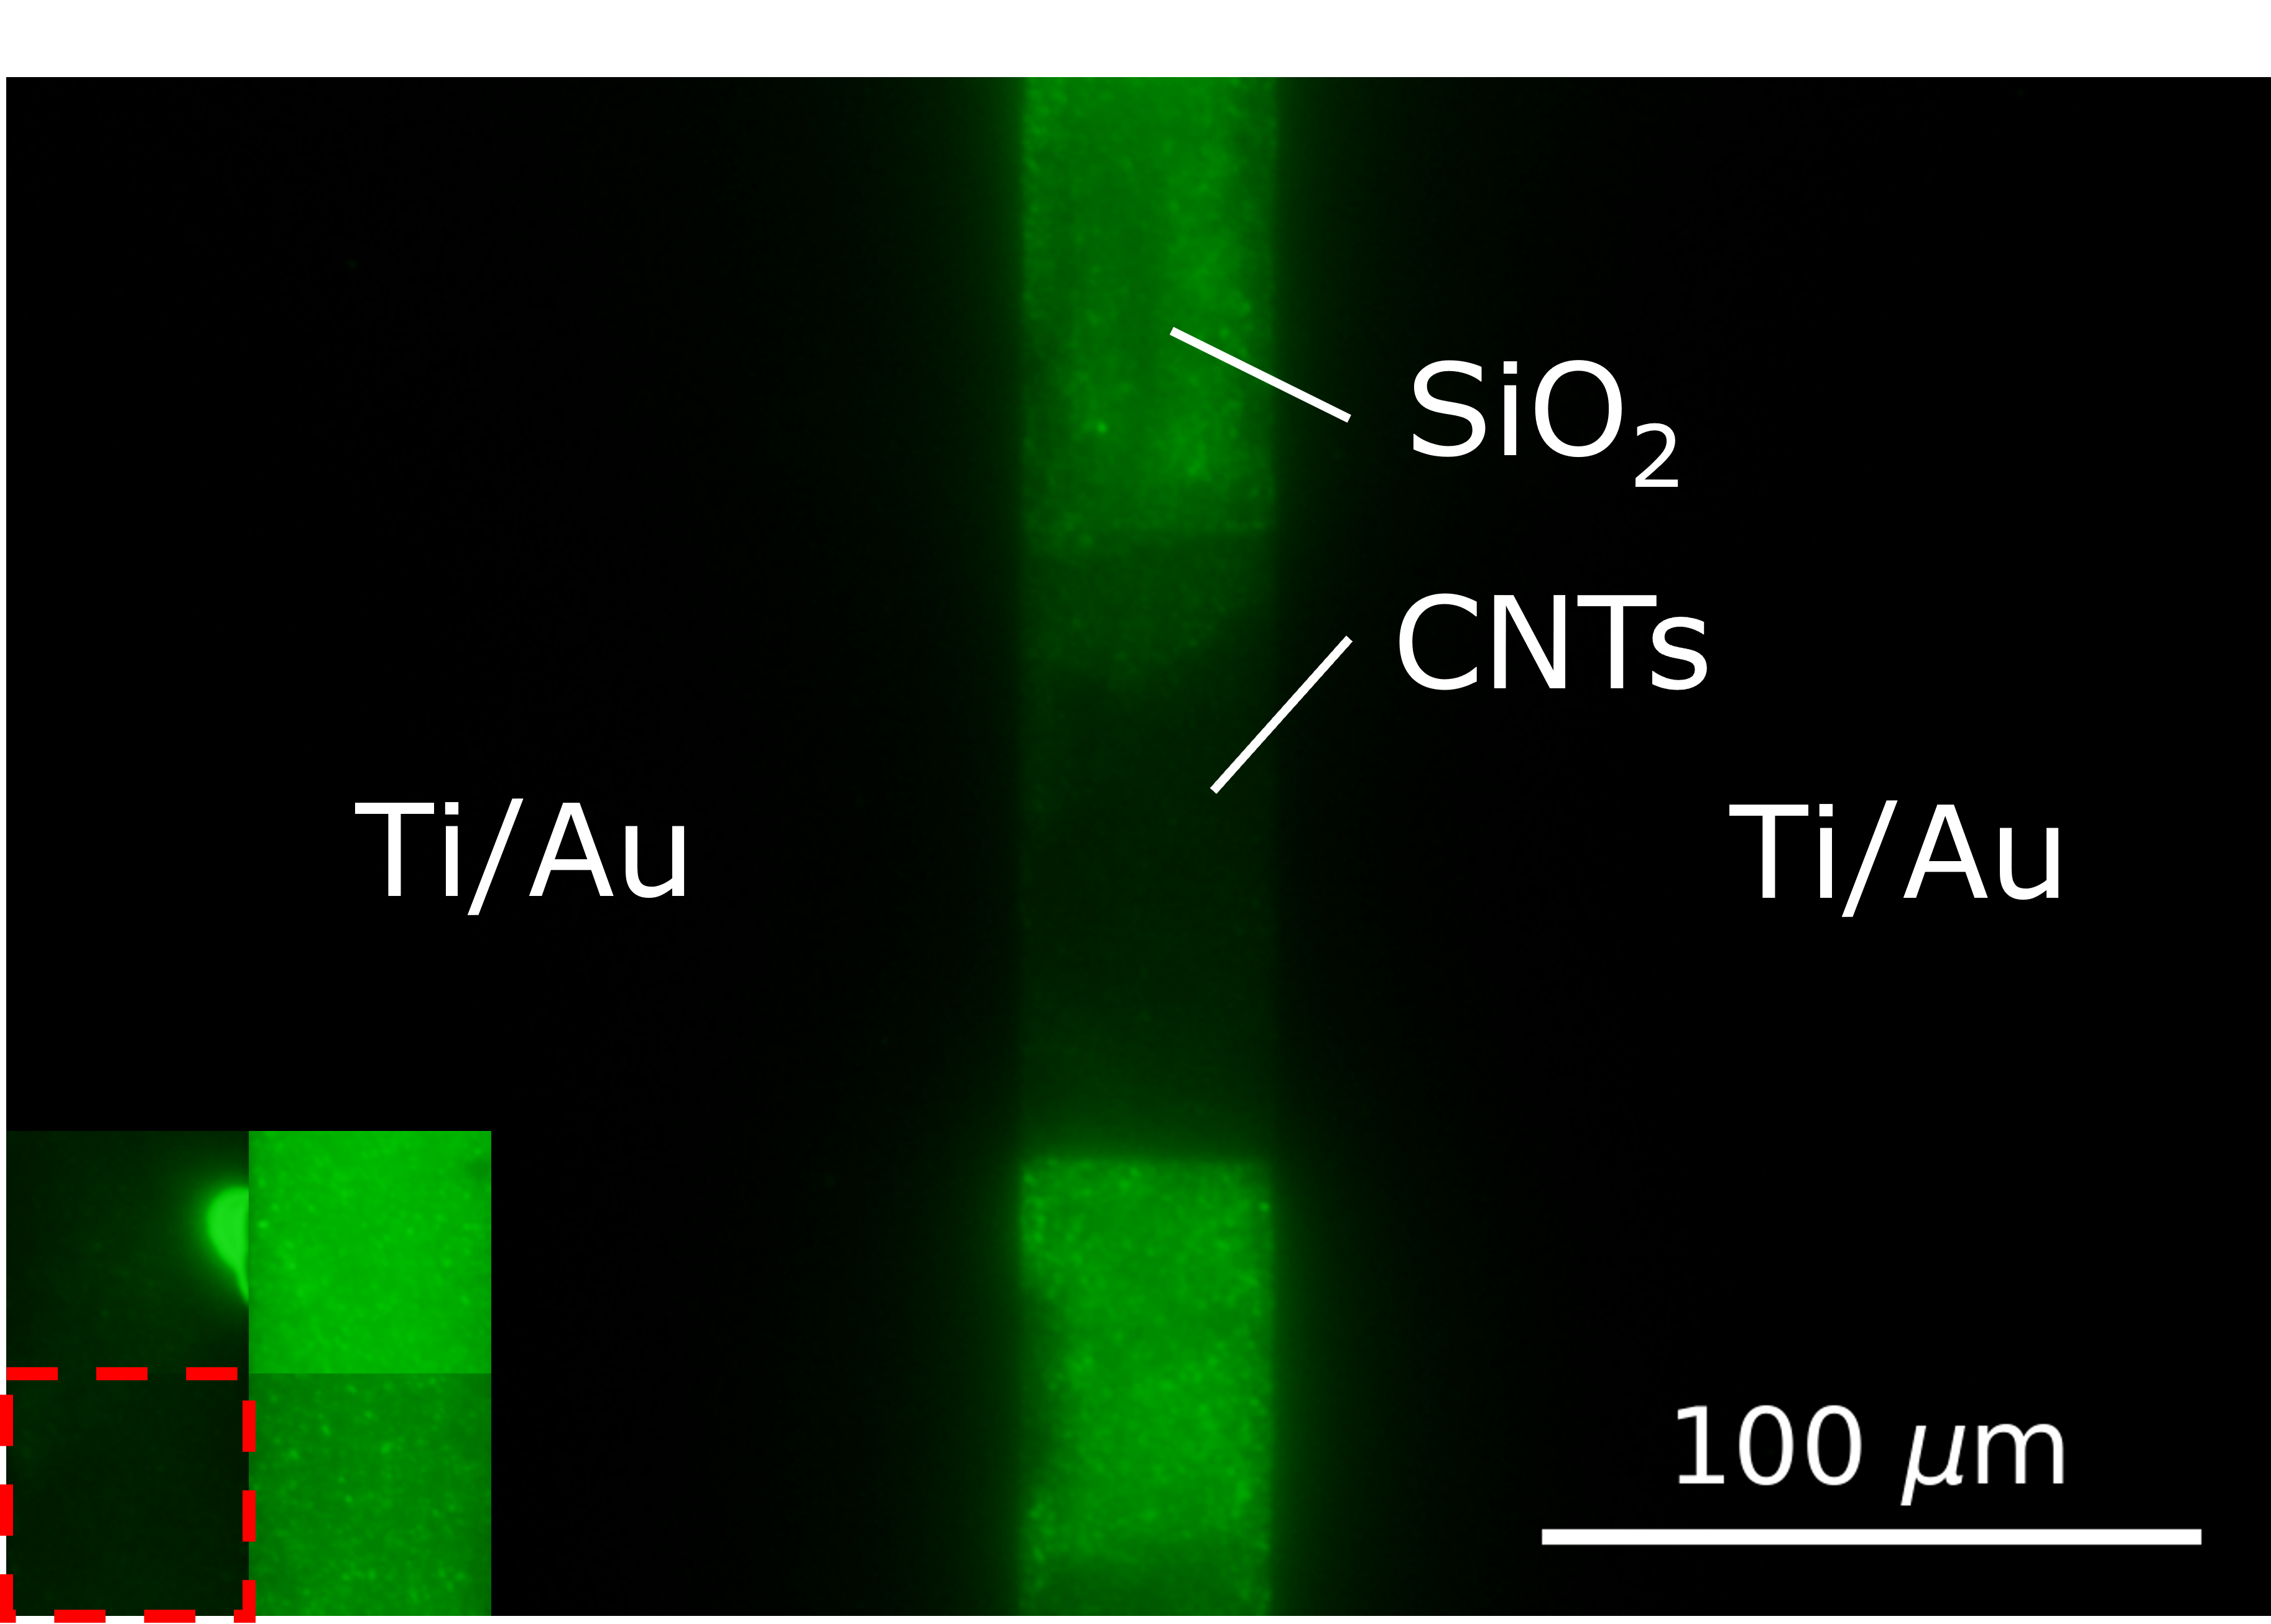
\includegraphics{figures/ch7/modified_GFPOR_10sexposure_40X_mediumcontrast_ch3_240208.png}

}

}

\subcaption{\label{fig-GFP-OR-ch3}}
\end{minipage}%
%
\begin{minipage}[t]{0.05\linewidth}

{\centering 

~

}

\end{minipage}%
%
\begin{minipage}[t]{0.47\linewidth}

{\centering 

\raisebox{-\height}{

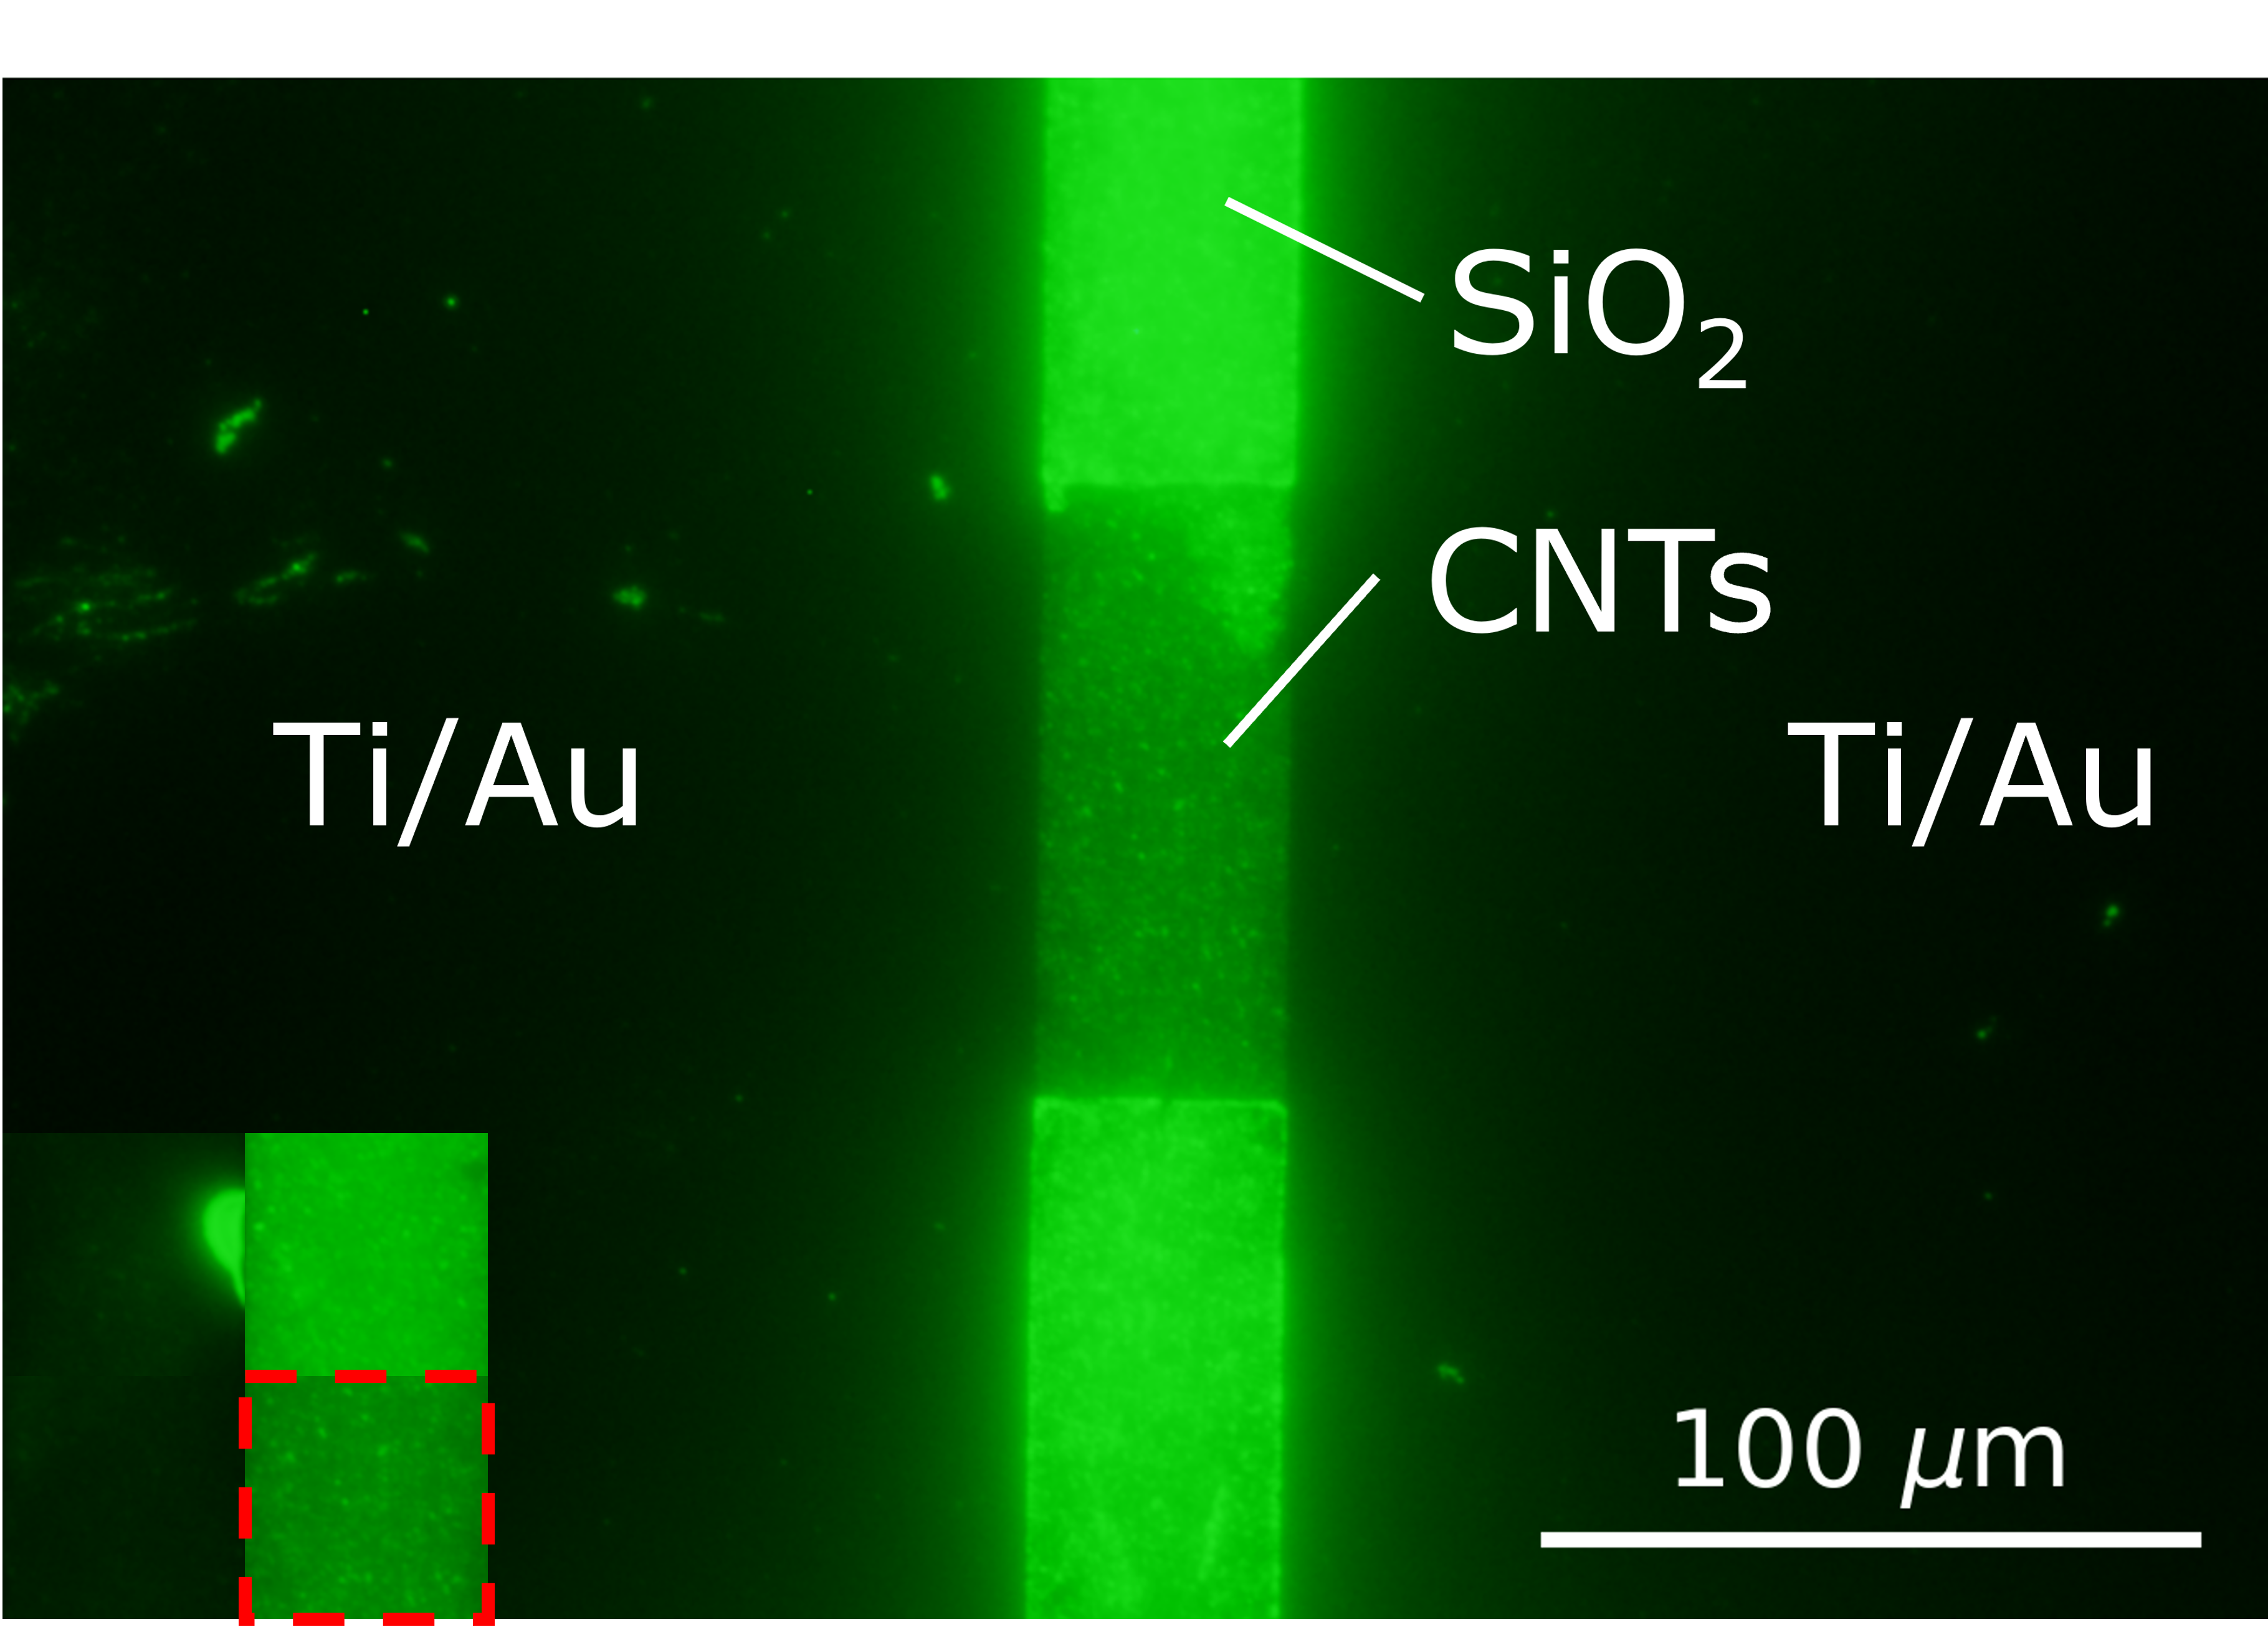
\includegraphics{figures/ch7/modified_GFPOR_PBASE_10sexposure_40X_mediumcontrast_ch2_231019.png}

}

}

\subcaption{\label{fig-PBASE-GFP-OR-ch2}}
\end{minipage}%

\caption{\label{fig-PBASE-GFP-ORs}The fluorescence images on the left
side \(-\) (a), (c) and (e) \(-\) show unencapsulated carbon nanotube
network channels from a device incubated in GFP-OR43b nanodiscs. The
fluorescence images on the right \(-\) (b), (d) and (f) \(-\) show the
channels of a similar device after successive PBASE and GFP-OR43b
nanodisc incubation. Images (a) and (c) are both of the same channel on
the first device, and images (b) and (d) are of the same channel on the
second, but (c) and (d) were taken using a greater magnification. The
insets in (c)-(f) compare the central channel region of (c)-(f) more
directly. All images were taken using the same microscope settings, with
a GFP filter and a 10 s exposure time.}

\end{figure}

The functionalisation of unencapsulated carbon nanotube devices
(steam-deposited, fabricated using post-June 2023 methods outlined in
\textbf{?@sec-fabrication}) with PBASE and GFP-OR nanodiscs was
performed as follows:

\begin{enumerate}
\def\labelenumi{\arabic{enumi}.}
\item
  The device was exposed to UV light for 1 minute, placed in
  AZ\(^\circledR\) 326 developer for 3 minutes, then rinsed with
  acetone, isopropanol and nitrogen dried.
\item
  The device was vacuum annealed for 1 hour at 150°C (Note: Steps 1 \& 2
  were added to ensure any residual photoresist on the channel was
  removed or passivated before functionalisation, see
  Section~\ref{sec-photoresist-contamination}).
\item
  A solution of 1 mM PBASE (Setareh Biotech) in methanol prepared by
  fully dissolving 2 mg PBASE in 5 mL methanol by vortex mixing at 1000
  rpm in a dark room (Note: PBASE was stored at -18°C for 18 months
  prior to use, and was thawed under vacuum for 15 minutes in dark
  conditions before opening)
\item
  The device was then rinsed with methanol, fully submerged in \(\sim\)
  1 mL of PBASE in methanol solution and left covered with parafilm for
  1 hour, then rinsed with methanol for 15 s, rinsed with 1XPBS for 15 s
  and nitrogen dried to remove residual PBASE.
\item
  The device was left dry and in darkness while collecting the GFP-OR
  nanodiscs from the -80°C freezer.
\item
  20 \(\mu\)L GFP-OR nanodiscs (batch number ND-GFP-OR43b-0002, prepared
  12 months earlier) were diluted in 2 mL 1XPBS (Note: The full 2 mL was
  used to flush out the nanodisc vial when preparing the nanodisc
  solution, with successive additions and subtractions of 50 \(\mu\)L
  1XPBS into and from the vial).
\item
  The device was submerged in the GFP-OR43b nanodisc solution and left
  covered with parafilm for 1 hour, then rinsed with 1XPBS for 15 s.
\item
  For fluorescence microscopy, the device was briefly rinsed with DI
  water and nitrogen dried to remove dried-down salt residue left by the
  1XPBS.
\item
  Fluorescence microscope images were taken immediately after
  functionalisation; devices were transported to the fluorescence
  microscope room in a foil-wrapped container, and the fluorescence
  microscope room was kept dark while images were taken.
\end{enumerate}

A control device was prepared using the same process but skipping steps
3 and 4. Fluorescence images of both devices are shown in
Figure~\ref{fig-PBASE-GFP-ORs}. All fluorescence images were taken of
channels with a measured resistance within a 50-500 k\(\Omega\) range
both before and after functionalisation.

As mentioned in \textbf{?@sec-fluorescence-characterisation}, the
rectangular dark regions to the left and right of each image are the
gold electrodes. The silicon dioxide regions in each image appear bright
under the GFP filter, indicating non-specific binding between the
GFP-OR43b nanodiscs and the silicon dioxide substrate. As this device
has been annealed, UV exposed and developed before functionalisation,
this non-specific attachment is unlikely to be interaction with residual
photoresist (see Section~\ref{sec-photoresist-contamination}). The
SiO\(_2\) substrate also appears brighter in the images on the right of
Figure~\ref{fig-PBASE-GFP-ORs}, which are of the device initially
exposed to PBASE. The discussion in
Section~\ref{sec-pyrene-interactions} indicates that the pyrene moiety
of PBASE may non-specifically interact with the silicon dioxide
substrate, therefore, the SiO\(_2\) substrate may have had a coating of
attached PBASE when the device on the right of
Figure~\ref{fig-PBASE-GFP-ORs} was submerged in the GFP-OR43b nanodiscs.
The attachment of GFP-OR43b nanodiscs to this PBASE coating may have
been more extensive than direct attachment of GFP-OR43b nanodiscs to the
silicon dioxide, which led to brighter fluorescence of the modified
silicon dioxide for the PBASE-incubated device.

A comparison of fluorescence in the channel region between images on the
left of Figure~\ref{fig-PBASE-GFP-ORs} (GFP-OR43b only) and the images
on the right (GFP-OR43b and PBASE) is given by the inset in
Figure~\ref{fig-GFP-OR-ch6}-f.~The inset demonstrates that the channels
not incubated in PBASE are significantly less bright than those that had
been incubated with PBASE. It appears that, as expected from the
discussion in Section~\ref{sec-hydrophobicity}, the GFP-OR43b in 1XPBS
is unable to approach the unmodified channel due to the hydrophobicity
of the carbon nanotubes. However, when the carbon nanotubes are modified
with PBASE, the GFP-OR43b is able to attach to the channel, and so the
channel shows up brightly under the fluorescence microscope GFP filter.
This trend was consistent across all conducting channels on each of the
two devices.

\hypertarget{sec-conclusion}{%
\subsection{Conclusion}\label{sec-conclusion}}

It has been well-established in the literature that the \(\pi\)-stacking
reaction mechanism between pyrene-based linkers and graphene and carbon
nanotube network field-effect transistors can be used to create working
biosensors. The previous use of various linker molecules for biosensor
functionalisation was investigated. Despite the wide use of
1-pyrenebutanoic acid N-hydroxysuccinimide ester (PBASE) and
1-pyrenebutyric acid (PBA) for functionalisation of biosensors, the
literature shows a significant variation in the methods used for
attachment of linker molecules to a transistor channel. The most common
methods, using 6 mM PBASE dissolved in dimethylformamide or 1 mM PBASE
in methanol, stem directly from the first documented use of PBASE for
functionalisation of carbon nanotube biosensors. In the last 6 years,
more research has been done into optimising the PBASE methodology for
graphene devices, but there is still disagreement in the literature over
whether minimising or maximising PBASE coverage on a graphene device
channel is desirable for sensing. Due to disagreement in the literature
around suitable non-covalent methods for biosensor functionalisation,
several steps were taken to identify a rapid and simple method for
verifying successful functionalisation, and to locate any potential
barriers to a successful functionalisation.

I first compared the advantages and disadvantages of the various linker
molecules under investigation. The use of hydrogen NMR gave indications
that water was present in PBASE samples prepared in DMSO. Concerns
around the impact of the hydrolysis of PBASE on functionalisation mean
that the presence of water is strongly undesirable. An alternative
functionalisation approach less prone to hydrolysis is the reaction of
PBA with EDC in the presence of NHS. However, this process has its own
disadvantages, such as undesirable protein interactions and the
increased amount of steps and process variables involved. Pyrene-NTA is
also less prone to hydrolysis than PBASE but unlike PBASE or PBA/EDC
interacts with a specific protein tag, the histidine tag. PEGlyation of
the pyrene-NTA linker also means that the entire functionalisation
process can be performed in aqueous solution, avoiding the introduction
of non-organic solvents. This approach is desirable, since the
non-aqueous solvents traditionally used for functionalisation may have
negative impacts on device behaviour. For example, carbon nanotube
device channel transfer characteristics were found to undergo a
significant shift of \(\Delta V = -0.15 \pm 0.02\) when exposed to DMSO
or MeOH for 1 hour.

Next, I verified that the pyrene groups of the linker molecules of
interest were attaching successfully to either carbon nanotubes or
graphene. Raman spectroscopy showed that incubating a highly-bundled
carbon nanotube film in 5 mM PBASE or PBA in DMSO for 1 hour increased
I\(_D\)/I\(_G\) by a factor of \(\sim 3\) relative to the DMSO-only
case. Incubating a steam-deposited carbon nanotube device in a 1 mM
concentration of PBASE in methanol or DMSO for 1 hour was found to cause
a significant increase in device on-current relative to the solvent-only
case, and a similar increase in on-current was seen for 5 mM PBA in DMSO
relative to the DMSO-only case. When a PBA-functionalised device was
placed in aqueous solution with 20 mM EDC and 40 mM NHS for 30 minutes,
a further increase in on-current was seen. Fluorescence microscopy was
used to demonstrate the successful attachment of pyrene-PEG to graphene
using an attached FITC probe, where immersing a graphene film in 1 mM
pyrene-PEG in ethanol led to the channels becoming brightly fluorescent
relative to the background using a 1 s exposure time.

Various obstacles to successful functionalisation were encountered and
addressed. Photoresist contamination was addressed with exposure and
development steps before functionalisation (no exposure for SU8
encapsulated devices). Hydrophobicity of graphene films was addressed by
plasma treatment before functionalisation in aqueous solution. A
surfactant rinse was used to distinguish between weak substrate-linker
interaction and \(\pi\)-stacking between linker and the channel.
Finally, coffee-ring distribution of linker was addressed by always
submerging the device in linker when functionalising.

Finally, fluorescence microscopy was used to investigate PBASE
functionalisation of GFP-tagged odorant receptors. An eight-channel
device was modified by submersion in 1 mM PBASE in methanol for 1 hour,
then submersion in 10 \(\mu\)L mL\(^{-1}\) OR43b nanodiscs in 1XPBS for
1 hour. An eight-channel control device was also prepared by submersion
in 10 \(\mu\)L mL\(^{-1}\) OR43b nanodiscs in 1XPBS for 1 hour, but with
no PBASE. The channels of the PBASE-submersed devices showed significant
GFP fluorescence, while the channels of the control devices showed
little to no GFP fluorescence. As far as I am aware, this is the first
time fluorescence has been used to verify successful attachment of
odorant receptors to a carbon nanotube network.



\end{document}
